\documentclass[a4paper, 12pt]{article}
\UseRawInputEncoding
\title{Python}
\author{Biagio Spada}
\date{May 2025}
\UseRawInputEncoding


% Pacchetti per lingua e codifica
\usepackage[italian]{babel}    % Supporto per la lingua italiana
\usepackage[utf8]{inputenc}    % Supporto per i caratteri UTF-8
\usepackage[T1]{fontenc}       % Codifica dei font


% Pacchetti matematici
\usepackage{amsmath}           % Per formule matematiche
\usepackage{amssymb}           % Simboli matematici aggiuntivi

% Pacchetti per layout e struttura
\usepackage[margin=1.5cm]{geometry} % Margini personalizzati
\usepackage{fancyhdr}          % Per intestazioni e piè di pagina
\usepackage{titlesec}          % Personalizzazione titoli
\usepackage{enumitem}          % Per personalizzare elenchi
\usepackage{float}             % Posizionamento preciso
\usepackage{tabularx}          % Tabelle avanzate
\usepackage{nameref}           % Riferimenti per nome
\usepackage{pdfpages}          % Inclusione di PDF
\usepackage{tcolorbox}         % Per creare box colorati
\tcbuselibrary{breakable,skins} % Estensioni per tcolorbox

% Pacchetti grafici
\usepackage{graphicx}          % Per includere immagini
\usepackage{tikz}              % Disegni vettoriali
\usetikzlibrary{shapes,arrows,positioning,shadows} % Estensioni per tikz
\usepackage{xcolor}            % Gestione avanzata dei colori

% Pacchetti per il codice
\usepackage{listings}          % Per inserire blocchi di codice

% Hyperref (caricato alla fine per evitare conflitti)
\usepackage{hyperref}          % Per link ipertestuali



\usepackage{booktabs}     % Per linee orizzontali professionali
\usepackage{siunitx}
\usepackage{colortbl}     % Per colorare le celle
\usepackage{array}
\usepackage{caption} 
\captionsetup[table]{font=bf, labelfont=bf}  % Bold caption
\renewcommand{\arraystretch}{1.4}  % Increase row spacing for readability\textbf{}
\usepackage{ragged2e} % Per un migliore allineamento del testo nelle celle (es. \RaggedRight)

% Configurazioni di pagina
\pagestyle{plain}              

% Personalizzazione del formato dei capitoli
\titleformat{\chapter}[display]
{\normalfont\huge\bfseries\color{blue!70!black}}
{\chaptertitlename\ \thechapter}{20pt}{\Huge}
[\vspace{2ex}\hrule\vspace{1ex}]

% Personalizzazione delle sezioni
\titleformat{\section}
{\normalfont\Large\bfseries\color{blue!60!black}}
{\thesection}{1em}{}
[\vspace{1ex}\hrule height 0.5pt\vspace{1ex}]

% Personalizzazione delle sottosezioni
\titleformat{\subsection}
{\normalfont\large\bfseries\color{blue!50!black}}
{\thesubsection}{1em}{}

% Definizione di stili per tikz
\tikzstyle{variable}=[draw, fill=blue!20, minimum width=2cm, minimum height=0.8cm, font=\bfseries, text centered]
\tikzstyle{memory}=[draw, fill=green!20, minimum width=3.5cm, minimum height=1.2cm, rounded corners, font=\bfseries, align=center]
\tikzstyle{reference}=[->, thick, blue]
\tikzstyle{label}=[font=\small\bfseries]
\tikzstyle{section title}=[font=\bfseries\large, text centered, text width=12cm]
\tikzstyle{subsection title}=[font=\bfseries, text centered, text width=10cm]
\tikzstyle{explanation}=[text width=12cm, align=center, font=\small]
\tikzstyle{id label}=[font=\small, text centered]

% Definizione colori per codice
\definecolor{codegreen}{rgb}{0,0.6,0}
\definecolor{codegray}{rgb}{0.5,0.5,0.5}
\definecolor{codepurple}{rgb}{0.58,0,0.82}
\definecolor{backcolour}{rgb}{0.95,0.95,0.95}

% Stile per codice Python
\lstdefinestyle{pythonstyle}{
    backgroundcolor=\color{backcolour},   
    commentstyle=\color{codegreen},
    keywordstyle=\color{orange},
    numberstyle=\tiny\color{codegray},
    stringstyle=\color{codepurple},
    basicstyle=\ttfamily\footnotesize,
    breakatwhitespace=true,         
    breaklines=true,                 
    captionpos=b,                    
    keepspaces=true,                 
    numbers=left,                    
    numbersep=5pt,                  
    showspaces=false,                
    showstringspaces=false,
    showtabs=false,                  
    tabsize=2,
    language=Python,
    xleftmargin=0.04\textwidth,
    xrightmargin=0.04\textwidth,
    linewidth=1.1\textwidth,
    postbreak=\mbox{\textcolor{red}{$\hookrightarrow$}\space},
    breakindent=0pt,
    columns=flexible,
    commentstyle=\color{codegreen}\raggedright,
}


% Definizione dei colori per una migliore leggibilità
\definecolor{setA}{RGB}{255,182,193}      % Rosa chiaro per insieme A
\definecolor{setB}{RGB}{173,216,230}      % Azzurro chiaro per insieme B  
\definecolor{intersection}{RGB}{221,160,221} % Viola chiaro per intersezione
\definecolor{union}{RGB}{255,228,196}     % Pesca per unione completa


% Configurazione unificata per listings
\lstset{style=pythonstyle}
\lstset{
breaklines=true,             % Permetti il ritorno a capo per il codice
breakatwhitespace=true,      % Ritorna a capo solo agli spazi bianchi
style=pythonstyle,
postbreak=\mbox{\textcolor{red}{$\hookrightarrow$}\space}, % Indicatore di continuazione
breakindent=0pt,             % Nessuna indentazione dopo il ritorno a capo
columns=flexible,            % Spaziatura flessibile
keepspaces=true,             % Mantieni gli spazi
commentstyle=\color{codegreen}\raggedright, % Impedisci il ritorno a capo nei commenti
inputencoding=utf8,          % Specifica l'encoding di input
extendedchars=true,          % Supporto per caratteri estesi
literate={à}{{`a}}1         % Sostituisce 'à' con il comando LaTeX equivalente
{è}{{e'}}1         % Sostituisce 'è' con il comando LaTeX equivalente
{ì}{{`\i}}1        % Sostituisce 'ì' con il comando LaTeX equivalente
{ò}{{o'}}1         % Sostituisce 'ò' con il comando LaTeX equivalente
{ù}{{u'}}1         % Sostituisce 'ù' con il comando LaTeX equivalente
}

% Ambienti personalizzati
\newenvironment{chapterintro}
{\begin{tcolorbox}[
    enhanced,
    colback=blue!5!white,
    colframe=blue!75!black,
    arc=0mm,
    boxrule=0.5mm,
    left=5mm,
    right=5mm,
    top=5mm,
    bottom=5mm
]}
{\end{tcolorbox}}

\newenvironment{esempio}{\begin{tcolorbox}[colback=blue!5!white,colframe=blue!75!black,title=Esempio]}{\end{tcolorbox}}

\newtcolorbox{nota}[1][]{
    breakable,
    title=Nota,
    colback=blue!5,
    colframe=blue!75!black,
    fonttitle=\bfseries,
    #1
}

\newtcolorbox{ese}[1][]{
    breakable,
    title=Esempio,
    colback=green!5,
    colframe=green!75!black,
    fonttitle=\bfseries,
    #1
}

\newtcolorbox{attenzione}[1][]{
    breakable,
    title=Attenzione,
    colback=red!5,
    colframe=red!75!black,
    fonttitle=\bfseries,
    #1
}

% Comandi personalizzati
\newcommand{\sectionsep}{
    \begin{center}
        \vspace{0.5cm}
        \textcolor{blue!70!black}{$\ast$ $\ast$ $\ast$}
        \vspace{0.5cm}
    \end{center}
}

\newcommand{\percorsoApprendimento}[2]{
\begin{center}
\begin{tikzpicture}
    \node[draw=blue!70!black, fill=blue!5, rounded corners, text width=0.85\textwidth, inner sep=10pt, drop shadow] {
        \textbf{Percorso di apprendimento:} #1
        
        \vspace{0.3cm}
        #2
    };
    % Aggiungi un indicatore grafico di "continua"
    \node[right=0.1cm of current bounding box.east, font=\Large\bfseries, text=blue!70!black] {→};
\end{tikzpicture}
\end{center}
}


\begin{document}
\maketitle

\begin{abstract}
Questi appunti raccolgono i concetti fondamentali del linguaggio Python, con esempi pratici tratti da esercizi svolti personalmente. Il documento è stato creato come strumento di ripasso e per facilitare l'apprendimento di Python.

Gli argomenti trattati spaziano dai concetti base (variabili, tipi di dati, strutture di controllo) a quelli più avanzati (classi, gestione dei file, moduli, algoritmi e strutture dati). Per ogni concetto vengono forniti esempi di codice commentati e spiegazioni dettagliate.
\end{abstract}

\newpage
% Inserimento dell'indice
\tableofcontents
\newpage

%Primo Capitolo
\newpage

\section{Introduzione a Python}

Python è un linguaggio di programmazione di alto livello, interpretato, orientato agli oggetti, con una sintassi semplice ed elegante. La sua popolarità è dovuta alla facilità di apprendimento e alla versatilità che lo rende adatto a molteplici ambiti.

\subsection{Caratteristiche Principali}
    \begin{itemize}
        \item  \textbf{Leggibilità}: La sintassi progettata per essere chiara e leggibile
        \item   \textbf{Versatilità}: Adatto a diversi contesti (web, data science, automazione, ecc.)
        \item \textbf{Gestione automatica della memoria}: Non è necessario allocare o deallocare manualmente la memoria
    \end{itemize}

\subsection{Installazione}
Il primo passo da compiere per iniziare a programmare con Python è installarlo sul proprio sistema. Python è disponibile per tutti i principali sistemi operativi: Windows, macOS e Linux.
\subsubsection{Scelta della versione}
Attualmente esistono due versioni principali di Python: Python 2 e Python 3. Si consiglia vivamente di utilizzare Python 3, poiché Python 2 non è più supportato dal gennaio 2020 e molte librerie moderne funzionano esclusivamente con Python 3.
\subsubsection{Download e installazione}
\begin{itemize}
\item \textbf{Windows}:
\begin{enumerate}
\item Visita il sito ufficiale Python (\url{https://www.python.org/downloads/})
\item Scarica l'ultima versione di Python 3 (ad esempio Python 3.11.x)
\item Esegui il file di installazione scaricato
\item \textbf{Importante:} Nella finestra di installazione, seleziona la casella \texttt{Add Python to PATH} prima di procedere
\item Clicca su \texttt{Install Now} per un'installazione standard o \texttt{Customize installation} per opzioni avanzate
\end{enumerate}
\item \textbf{macOS}:
\begin{enumerate}
    \item Visita il sito ufficiale Python (\url{https://www.python.org/downloads/})
    \item Scarica l'ultima versione di Python 3 per macOS
    \item Apri il file .pkg scaricato e segui le istruzioni di installazione
    \item In alternativa, se utilizzi Homebrew, puoi installare Python con il comando \texttt{brew install python3}
\end{enumerate}

\item \textbf{Linux}:
\begin{enumerate}
    \item Molte distribuzioni Linux includono già Python preinstallato. Puoi verificare la versione con \texttt{python3 --version} dal terminale
    \item Su Ubuntu/Debian: \texttt{sudo apt update \&\& sudo apt install python3 python3-pip}
    \item Su Fedora: \texttt{sudo dnf install python3}
    \item Su Arch Linux: \texttt{sudo pacman -S python python-pip}
\end{enumerate}
\end{itemize}
\subsubsection{Verifica dell'installazione}
Dopo l'installazione, è importante verificare che Python sia stato installato correttamente:
\begin{enumerate}
\item Apri il terminale (Command Prompt o PowerShell su Windows, Terminal su macOS/Linux)
\item Digita \texttt{python --version} o \texttt{python3 --version}
\item Dovresti vedere in output la versione di Python installata, ad esempio \texttt{Python 3.11.4}
\end{enumerate}
\subsubsection{Gestione dei pacchetti con pip}
Python include un gestore di pacchetti chiamato pip, che permette di installare facilmente librerie aggiuntive. Per verificare che pip sia installato:
\begin{enumerate}
\item Dal terminale, esegui \texttt{pip --version} o \texttt{pip3 --version}
\item Dovresti vedere la versione di pip installata
\end{enumerate}
Per installare una libreria, usa il comando:
\begin{lstlisting}
pip install nome_libreria
\end{lstlisting}
\subsubsection{Ambienti virtuali}
Per i progetti più complessi, è consigliabile utilizzare ambienti virtuali per mantenere le dipendenze separate. Per creare un ambiente virtuale:
\begin{lstlisting}
Creazione dell'ambiente virtuale
python -m venv mio_ambiente
Attivazione dell'ambiente virtuale
Su Windows
mio_ambiente\Scripts\activate
Su macOS/Linux
source mio_ambiente/bin/activate
\end{lstlisting}
\subsubsection{Opzioni alternative}
Se preferisci non installare Python direttamente sul tuo sistema, puoi considerare:
\begin{itemize}
\item \textbf{Anaconda}: Una distribuzione Python che include molte librerie scientifiche (\url{https://www.anaconda.com/})
\item \textbf{Piattaforme online}:
\begin{itemize}
\item Google Colab: Per notebook Python eseguiti nel browser
\item Replit: Per sviluppo Python online
\item PythonAnywhere: Ambiente Python basato su cloud
\item Deepnote come Replit, ambiente di sviluppo online
\end{itemize}
\end{itemize}

\subsection{Il tuo primo programma Python}\label{primoProgramma}

Ecco un esempio classico per iniziare con Python che include sia l'output che l'input:

\begin{lstlisting}
# Il mio primo programma Python
print("Hello, World!")  # Stampa un messaggio a schermo

# Richiesta di input all'utente
nome = input("Come ti chiami? ")
print(f"Ciao {nome}, benvenuto nel mondo di Python!")
\end{lstlisting}

\begin{nota}
\textbf{Come eseguire il codice Python:}
\begin{enumerate}
    \item \textbf{Da terminale}: Salva il codice in un file con estensione .py (es. primo\_programma.py) e eseguilo con il comando \texttt{python primo\_programma.py}
    \item \textbf{Da IDE}: Usa un ambiente di sviluppo come PyCharm, Visual Studio Code o IDLE (incluso nell'installazione di Python)
    \item \textbf{Da notebook}: Jupyter Notebook permette di eseguire il codice in celle interattive
    \item \textbf{Online}: Servizi come replit.com o Google Colab permettono di scrivere ed eseguire codice Python senza installazioni
\end{enumerate}
\end{nota}




%Capitolo 2 Introduzione alle variabili in Python



\section{Variabili e Tipi di Dati}

\subsection*{Introduzione}
In questa sezione esploreremo il cuore della programmazione Python: variabili e tipi di dati. Vedremo come Python gestisce diversi tipi di informazioni, come memorizzarle in variabili, e come manipolarle attraverso varie operazioni. Comprenderemo le regole per denominare le variabili, come Python interpreta i diversi tipi di dati, e come interagiscono tra loro. 

In Python, le variabili sono contenitori per memorizzare valori di dati. A differenza di altri linguaggi di programmazione, Python non richiede di dichiarare esplicitamente il tipo di una variabile prima di usarla. Il tipo viene determinato automaticamente in base al valore assegnato.

\subsection{Dichiarazione e Assegnazione delle Variabili}\label{bestPractice}
\begin{lstlisting}
# Dichiarazione e assegnazione di variabili
nome = "Mario"      # Una stringa
eta = 30            # Un intero
altezza = 1.75      # Float
e_studente = False  # Booleano
\end{lstlisting}


\subsection{Regole e best practice per denominare le variabili}

In Python, i nomi delle variabili devono seguire regole precise e alcune convenzioni che rendono il codice più leggibile e manutenibile.

\begin{tcolorbox}[colback=blue!5!white,colframe=blue!75!black,title=Regole sintattiche]
\begin{itemize}[leftmargin=*,itemsep=0.5em]
    \item \textbf{Caratteri consentiti}: Lettere (a-z, A-Z), numeri (0-9) e underscore (\_)
    \item \textbf{Primo carattere}: Deve essere una lettera o un underscore, mai un numero
    \item \textbf{Case sensitivity}: \texttt{nome}, \texttt{Nome} e \texttt{NOME} sono tre variabili diverse
    \item \textbf{Parole riservate}: Non è possibile usare parole chiave di Python (come \texttt{if}, \texttt{for}, \texttt{while})
\end{itemize}
\end{tcolorbox}

\begin{tcolorbox}[colback=green!5!white,colframe=green!75!black,title=Convenzioni di stile (PEP 8)]
\begin{itemize}[leftmargin=*,itemsep=0.5em]
    \item \textbf{snake\_case}: Per variabili e funzioni (es. \texttt{nome\_utente})
    \item \textbf{SCREAMING\_SNAKE\_CASE}: Per costanti (es. \texttt{MAX\_TENTATIVI})
    \item \textbf{CamelCase}: Per classi (es. \texttt{PersonaUtente})
    \item \textbf{Nomi significativi}: Evitare sigle come \texttt{x}, \texttt{y}, preferire nomi descrittivi
    \item \textbf{Underscore iniziale}: \texttt{\_variabile} suggerisce uso interno o privato
\end{itemize}
\end{tcolorbox}

\begin{lstlisting}
# Esempi di nomi validi
nome = "Alice"
_eta = 25
nome_completo = "Alice Rossi"
variabile1 = 42
COSTANTE = 3.14159

# Esempi di nomi non validi
# 1variabile = 10    # Inizia con un numero (errore di sintassi)
# for = "ciclo"      # E una parola riservata (errore di sintassi)
# nome-utente = "Mario"  # Il trattino non e' consentito
\end{lstlisting}

\vspace{0.5cm}


\clearpage
\section{Metodi principali per i tipi di dati Python}

\subsection*{Cos'è un metodo in Python?}

In Python, i \textbf{metodi} sono funzioni speciali associate a oggetti di specifici tipi di dati. A differenza delle funzioni standard che accettano dati come argomenti, i metodi sono "collegati" agli oggetti stessi attraverso la notazione punto (\texttt{oggetto.metodo()}).

Ogni tipo di dato in Python possiede metodi specifici progettati per operazioni comuni e naturali su quel tipo. Questa caratteristica è parte fondamentale del paradigma della programmazione orientata agli oggetti che Python supporta.


\begin{lstlisting}[style=pythonstyle]
# Funzione standard
len("Python")  # 6

# Metodo
"Python".upper()  # "PYTHON"
\end{lstlisting}


\subsection*{Metodi e mutabilità}\label{MutabilitàImmutabilità}

Un concetto cruciale per comprendere i metodi in Python è la \textbf{mutabilità}. I tipi di dati in Python si dividono in due categorie:

\begin{itemize}
    \item \textbf{Tipi immutabili}: una volta creati, non possono essere modificati (stringhe, tuple, numeri)
    \item \textbf{Tipi mutabili}: possono essere modificati dopo la creazione (liste, dizionari, set)
\end{itemize}

Questa distinzione influenza profondamente il comportamento dei metodi:

\begin{tcolorbox}[colback=blue!5!white,colframe=blue!75!black,title=Comportamento dei Metodi]
\begin{tabularx}{\textwidth}{|l|X|}
\hline
\textbf{Tipi immutabili} & I metodi \textbf{restituiscono sempre} un nuovo oggetto, lasciando l'originale invariato \\
\hline
\textbf{Tipi mutabili} & I metodi spesso \textbf{modificano direttamente} l'oggetto (operazioni in-place) \\
\hline
\end{tabularx}
\end{tcolorbox}

\subsection*{Metodi delle stringhe}

Le stringhe (\texttt{str}) sono sequenze immutabili di caratteri, quindi i loro metodi restituiscono sempre nuove stringhe. Questi metodi consentono di trasformare e analizzare testo in modi potenti e flessibili.

La potenza dei metodi per stringhe si apprezza particolarmente nell'elaborazione del testo, dove possiamo concatenare più operazioni in sequenza:


\begin{lstlisting}[style=pythonstyle]
# Pulizia e parsing di dati testuali
testo_grezzo = "  python, java, C++  "
linguaggi = testo_grezzo.strip().lower().split(", ")
print(linguaggi)  # ['python', 'java', 'c++']
\end{lstlisting}




\subsection*{Principi guida per l'uso dei metodi}

Quando lavori con i metodi in Python, tieni a mente questi principi:

\begin{enumerate}
    \item \textbf{Verifica la mutabilità}: prima di usare un metodo, capisci se stai lavorando con un tipo mutabile o immutabile
    \item \textbf{Controlla il valore restituito}: alcuni metodi restituiscono un nuovo oggetto, altri modificano l'oggetto esistente
    \item \textbf{Leggi la documentazione}: quando sei in dubbio, consulta la documentazione ufficiale
\end{enumerate}

\begin{nota}
La documentazione ufficiale di Python (\url{https://docs.python.org/3/library/stdtypes.html}) contiene l'elenco completo di tutti i metodi disponibili per ciascun tipo di dato, con spiegazioni dettagliate ed esempi.
\end{nota}

Di seguito vengono riportate le tabelle con i principali metodi per la manipolazione delle stringhe in Python, si tratta di metodi preinstallati in Python:


% Stringhe (str)
\begin{table}[H]
\centering
\caption{Metodi essenziali per le stringhe (\texttt{str})}
\begin{tabularx}{\textwidth}{|l|X|l|}
\hline
\textbf{Metodo} & \textbf{Descrizione} & \textbf{Esempio} \\
\hline
\texttt{upper()} & Converte in maiuscolo & \texttt{"python".upper() → "PYTHON"} \\
\hline
\texttt{lower()} & Converte in minuscolo & \texttt{"Python".lower() → "python"} \\
\hline
\texttt{strip()} & Rimuove spazi agli estremi & \texttt{"  Python  ".strip() → "Python"} \\
\hline
\texttt{replace(old, new)} & Sostituisce le occorrenze & \texttt{"Hello".replace("l", "x") → "Hexxo"} \\
\hline
\texttt{split(sep)} & Divide in una lista & \texttt{"a,b,c".split(",") → ["a", "b", "c"]} \\
\hline
\texttt{join(iterable)} & Unisce una lista in stringa & \texttt{"-".join(["a", "b"]) → "a-b"} \\
\hline
\texttt{find(sub)} & Trova posizione sottostringa & \texttt{"Python".find("th") → 2} \\
\hline
\end{tabularx}
\end{table}






%Sottocapitolo degli Operatori
\clearpage
\subsection{Operatori}\label{Operatori}
In questa sottosezione andremo a visionare i principali Operatori presenti su Python, possiamo considerarli come "strumenti" che permettono di manipolare dati, eseguire calcoli e prendere decisioni all'interno del codice. Gli opreatori sono essenzialmente simboli speciale che indicano al computer di eseguire operazioni specifiche sui valori (o operandi) a cui sono applicati.

Alcuni di essi possono risultare alquanto ambigui per la loro essenza e semplicità ma rappresentano un valore chiave per la comprensione dell'azione che bisogna eseguire.


\begin{itemize}
    \item \textbf{Operatori aritmetici}: permettono di eseguire calcoli matematici sui numeri
    \item \textbf{Operatori di confronto}: consentono di comparare valori e restituiscono risultati booleani (vero o falso)
    \item \textbf{Operatori logici}: permettono di combinare condizioni booleane e sono essenziali nelle strutture decisionali
\end{itemize}


Accanto agli operatori, le funzionalità di input e output rappresentano le "porte" attraverso cui un programma comunica con l'utente o con l'ambiente esterno. Attraverso queste funzioni, i programmi possono acquisire dati, presentare risultati e interagire con chi li utilizza.

Gli esempi che seguono illustrano la sintassi e l'uso pratico di ciascun tipo di operatore e delle funzioni di input/output di base in Python.


\subsubsection{Operatori aritmetici}\label{operatoriMatemateci}
\begin{lstlisting}
a = 10
b = 3

somma = a + b          # 13
differenza = a - b     # 7
prodotto = a * b       # 30
divisione = a / b      # 3.3333... (divisione che restituisce float)
div_intera = a // b    # 3 (divisione intera)
modulo = a % b         # 1 (resto della divisione)
potenza = a ** b       # 1000 (a elevato alla b)
\end{lstlisting}

\subsubsection{Operatori di confronto}
\begin{lstlisting}
a == b    # Uguaglianza (False)
a != b    # Disuguaglianza (True)
a > b     # Maggiore (True)
a < b     # Minore (False)
a >= b    # Maggiore o uguale (True)
a <= b    # Minore o uguale (False)
\end{lstlisting}

\subsubsection{Operatori logici}\label{opLogici}
\begin{lstlisting}
x = True
y = False

x and y    # False (AND logico)
x or y     # True (OR logico)
not x      # False (NOT logico)
\end{lstlisting}


\subsection{Input e Output}\label{InputOutput}
\begin{lstlisting}
# Output sulla console
print("Ciao, mondo!")

# Input da tastiera
nome = input("Come ti chiami? ")
print(f"Ciao, {nome}!")

# Formattazione delle stringhe
eta = 25
messaggio = f"Ho {eta} anni."
print(messaggio)
\end{lstlisting}


%Capitolo Approfondimento delle Variabili
\clearpage

\section{Approfondimento delle Variabili}\label{variabiliMemoria}

\subsection{Il modello di riferimento in Python}

In Python, le variabili funzionano in modo diverso rispetto ad altri linguaggi di programmazione. Anziché essere "contenitori" che memorizzano direttamente un valore, le variabili Python sono meglio descritte come "etichette" o "nomi" che fanno riferimento a oggetti in memoria.

Per comprendere veramente questo concetto, visualizziamo come Python gestisce le variabili in memoria.

\begin{lstlisting}
# Creazione di una variabile
a = 5
\end{lstlisting}

Quando eseguiamo questa istruzione, ecco cosa succede:

\begin{center}
\begin{tikzpicture}
    % Riquadri con titoli
    \node[draw, rounded corners, fill=blue!5, minimum width=3cm, minimum height=3cm, label={[font=\bfseries]above:Variabile}] (var_box) at (0,0) {};
    
    \node[draw, rounded corners, fill=green!5, minimum width=3cm, minimum height=3cm, label={[font=\bfseries]above:Memoria}] (mem_box) at (4,0) {};
    
    % Variabile
    \node[draw, fill=blue!20, minimum width=2cm, minimum height=0.8cm] (var_a) at (0,0) {a};
    
    % Oggetto in memoria
    \node[draw, fill=green!20, minimum width=1.5cm, minimum height=1.5cm, rounded corners] (obj_5) at (4,0) {5};
    
    % Freccia di riferimento
    \draw[->, thick] (var_a) -- (obj_5);
\end{tikzpicture}
\end{center}

Python crea un oggetto intero con valore 5 in memoria e associa la variabile \texttt{a} a questo oggetto.\\ La variabile \texttt{a} non "contiene" 5, ma "punta a" o "fa riferimento a" l'oggetto 5 in memoria.

\subsection{Assegnazione di variabili}

Vediamo cosa succede quando creiamo una seconda variabile e le assegniamo il valore della prima:

\begin{lstlisting}
a = 5
b = a  # b ora fa riferimento allo stesso oggetto di a
\end{lstlisting}

\begin{center}
\begin{tikzpicture}
    % Riquadri di raggruppamento
    \node[draw, rounded corners, fill=blue!5, minimum width=3cm, minimum height=4cm, label={[font=\bfseries]above:Variabili}] (vars) at (0,0) {};
    \node[draw, rounded corners, fill=green!5, minimum width=3cm, minimum height=4cm, label={[font=\bfseries]above:Memoria}] (mem) at (4.5,0) {};
    
    % Variabili
    \node[draw, fill=blue!20, minimum width=2cm, minimum height=0.8cm] (var_a) at (0,1) {a};
    \node[draw, fill=blue!20, minimum width=2cm, minimum height=0.8cm] (var_b) at (0,-1) {b};
    
    % Oggetto in memoria
    \node[draw, fill=green!20, minimum width=1.5cm, minimum height=1.5cm, rounded corners] (obj_5) at (4.5,0) {5};
    
    % Frecce di riferimento
    \draw[->, thick] (var_a) -- (obj_5);
    \draw[->, thick] (var_b) -- (obj_5);
\end{tikzpicture}
\end{center}

Ora sia \texttt{a} che \texttt{b} fanno riferimento allo stesso oggetto in memoria. Non viene creata una copia del valore.

\subsection{Tipi immutabili vs mutabili}\label{mutableImmutable}
    In Python, la distinzione tra tipi di dati mutabili e immutabili rappresenta uno dei concetti fondamentali che influenzano profondamente il comportamento del codice. Questa distinzione, apparentemente semplice, ha implicazioni significative sulla manipolazione dati, sull'ottimizzazione della memoria.

    \subsubsection*{La natura dell'immutabilità e della mutabilità}
    Quando parliamo di \textbf{immutabilità}, ci riferiamo a oggetti che, una volta creati, non possono essere modificati nel loro stato interno. Qualsiasi opeazione sembra modificare un oggetto immutabile in realtà crea un nuovo oggetto con i valori aggiornati. È come se questi oggetti portassero con sé un cartello invisibile che dice: "Guardami, ma non toccarmi".
    Al contrario, gli oggetti mutabili possono essere alterati dopo la loro creazione. Il loro stato interno può cambiare mentre l'identità dell'oggetto rimane la stessa. Possiamo pensare agli oggetti mutabili come a contenitori il cui contenuto può essere modificato, rimosso o sostituito senza dover sostituire l'intero contenitore.

    \subsubsection*{La classificazione In Python}
    Python organizza i suoi tipi di dati nativi in queste due categorie:

    \begin{itemize}
        \item \textbf{Tipi Immutabili:}
        \begin{itemize}
            \item \textbf{Numeri} (\textit{int, float, complex})
            \item \textbf{Stringe} (\textit{str})
            \item \textbf{Tuple} (\textit{tuple})
            \item \textbf{Frozen sets} (\textit{frozenset})
            \item \textbf{Booleani} (\textit{bool})
            \item \textbf{None} (\textit{NoneType})
        \end{itemize}
    \end{itemize}

    \begin{itemize}
        \item \textbf{Tipi Mutabili:}
        \begin{itemize}
            \item \textbf{Liste} (\textit{list})
            \item \textbf{Dizionari} (\textit{dict})
            \item \textbf{Set} (\textit{set})
        \end{itemize}
    \end{itemize}

    \subsubsection*{Un modello concettuale}
    Per comprendere meglio questa distinzione, possiamo utilizzare un'analogia:

    Gli oggetti \textbf{immutabili} sono come documenti stampati su carta: se desideri modificare una parola, devi creare un nuovo documento. Non puoi alterare l'originale senza lasciare tracce evidenti.

    Gli oggetti \textbf{mutabili} sono invece come documenti digitali prima della stampa, alla quale puoi ancora aggiungere, eliminare o modificare i contenuti, mantenendo lo stesso file.
\vspace{0,5cm}
    

\begin{tcolorbox}[colback=blue!5!white,colframe=blue!75!black,title=Differenza tra tipi immutabili e mutabili]\label{TabellaMutabilitàImmutabilità}
In Python, la distinzione tra tipi immutabili e mutabili è fondamentale per comprendere il comportamento delle variabili:

\begin{itemize}[leftmargin=*,itemsep=0.5em]
    \item \textbf{Tipi immutabili} (non modificabili dopo la creazione):
    \begin{itemize}
        \item \texttt{int}: Numeri interi
        \item \texttt{float}: Numeri in virgola mobile
        \item \texttt{bool}: Valori booleani (True/False)
        \item \texttt{str}: Stringhe di testo
        \item \texttt{tuple}: Sequenze immutabili di elementi
        \item \texttt{frozenset}: Insiemi immutabili
    \end{itemize}
    
    \item \textbf{Tipi mutabili} (modificabili dopo la creazione):
    \begin{itemize}
        \item \texttt{list}: Liste di elementi
        \item \texttt{dict}: Dizionari (coppie chiave-valore)
        \item \texttt{set}: Insiemi di elementi unici
    \end{itemize}
\end{itemize}

Questa distinzione influenza profondamente come le variabili si comportano quando vengono assegnate, passate a funzioni o modificate.
\end{tcolorbox}

\subsubsection{Comportamento con tipi immutabili}

Quando lavoriamo con tipi immutabili, qualsiasi operazione che sembra modificare il valore in realtà crea un nuovo oggetto in memoria:

\begin{lstlisting}
a = 5
b = a
a = 10  # Questo NON modifica l'oggetto originale, ma crea un nuovo riferimento
print(b)  # Output: 5 (b continua a riferirsi all'oggetto originale)
\end{lstlisting}
\subsubsection{Comportamento con tipi mutabili}

I tipi mutabili come le liste si comportano diversamente:

\begin{lstlisting}
lista_a = [1, 2, 3]
lista_b = lista_a
lista_a.append(4)  # Questo modifica l'oggetto originale a cui puntano entrambe le variabili
\end{lstlisting}

Stato iniziale:
\begin{center}
\begin{tikzpicture}
    % Variabili
    \node[draw, fill=blue!20, minimum width=2cm, minimum height=0.8cm] (var_a) at (0,1) {lista\_a};
    \node[draw, fill=blue!20, minimum width=2cm, minimum height=0.8cm] (var_b) at (0,-1) {lista\_b};
    
    % Oggetto in memoria
    \node[draw, fill=green!20, minimum width=3cm, minimum height=1.5cm, rounded corners] (obj_list) at (4,0) {[1, 2, 3]};
    
    % Frecce di riferimento
    \draw[->, thick] (var_a) -- (obj_list);
    \draw[->, thick] (var_b) -- (obj_list);
\end{tikzpicture}
\end{center}

Dopo \texttt{lista\_a.append(4)}:
\begin{center}
\begin{tikzpicture}
    % Variabili
    \node[draw, fill=blue!20, minimum width=2cm, minimum height=0.8cm] (var_a) at (0,1) {lista\_a};
    \node[draw, fill=blue!20, minimum width=2cm, minimum height=0.8cm] (var_b) at (0,-1) {lista\_b};
    
    % Oggetto in memoria modificato
    \node[draw, fill=green!20, minimum width=3.5cm, minimum height=1.5cm, rounded corners] (obj_list) at (4,0) {[1, 2, 3, 4]};
    
    % Frecce di riferimento
    \draw[->, thick] (var_a) -- (obj_list);
    \draw[->, thick] (var_b) -- (obj_list);
\end{tikzpicture}
\end{center}

In questo caso, \texttt{lista\_a.append(4)} modifica direttamente l'oggetto lista in memoria. Poiché sia \texttt{lista\_a} che \texttt{lista\_b} puntano allo stesso oggetto, entrambe "vedono" la modifica.

\subsection{Verifica dell'identità degli oggetti}

Python fornisce due operatori per confrontare le variabili:

\textit{consultare per ripasso la sezione degli Operatori logici: \textbf{\nameref{opLogici}}}
\begin{itemize}
    \item \texttt{==} confronta i valori (uguaglianza)
    \item \texttt{is} confronta le identità (se le variabili puntano allo stesso oggetto)
\end{itemize}

\begin{lstlisting}
a = [1, 2, 3]
b = [1, 2, 3]  # Una nuova lista con gli stessi valori
c = a          # Riferimento alla stessa lista

print(a == b)  # True (stesso valore)
print(a is b)  # False (oggetti diversi)
print(a is c)  # True (stesso oggetto)

# Possiamo verificare l'identita anche con id()
print(id(a))  # Un numero unico che identifica l'oggetto
print(id(b))  # Un numero diverso
print(id(c))  # Stesso numero di id(a)
\end{lstlisting}

\begin{center}
\begin{tikzpicture}
    % Variabili
    \node[draw, fill=blue!20, minimum width=2cm, minimum height=0.8cm] (var_a) at (0,2) {a};
    \node[draw, fill=blue!20, minimum width=2cm, minimum height=0.8cm] (var_b) at (0,0) {b};
    \node[draw, fill=blue!20, minimum width=2cm, minimum height=0.8cm] (var_c) at (0,-2) {c};
    
    % Oggetti in memoria
    \node[draw, fill=green!20, minimum width=3cm, minimum height=1.5cm, rounded corners] (obj_list1) at (4,1) {[1, 2, 3]};
    \node[draw, fill=green!20, minimum width=3cm, minimum height=1.5cm, rounded corners] (obj_list2) at (4,-1) {[1, 2, 3]};
    
    % Frecce di riferimento
    \draw[->, thick] (var_a) -- (obj_list1);
    \draw[->, thick] (var_b) -- (obj_list2);
    \draw[->, thick] (var_c) to [out=0,in=180] (obj_list1);
    
    % IDs
    \node[above] at (obj_list2.north) {id: 4558921616};
    \node[above] at (obj_list1.north) {id: 4558921424};
\end{tikzpicture}
\end{center}

\subsection{Esercizio pratico: tracciare le variabili}

Esaminiamo un esercizio completo che mostra come tracciare le variabili in Python. Prevedere l'output di questo programma richiede di comprendere come Python gestisce i riferimenti in memoria.

\begin{lstlisting}
# Stato iniziale
x = 10
y = x
lista = [1, 2]
dizionario = {'a': 1, 'b': 2}

# Modifichiamo le variabili
x = 20
lista.append(3)
dizionario['c'] = 3

# Verifichiamo lo stato finale
print(x)        # Output: 20
print(y)        # Output: 10
print(lista)    # Output: [1, 2, 3]
print(dizionario)  # Output: {'a': 1, 'b': 2, 'c': 3}
\end{lstlisting}

Visualizziamo lo stato della memoria in diversi momenti dell'esecuzione:

\textbf{Stato iniziale:}
\begin{center}
\begin{tikzpicture}
    % Etichette per le sezioni con maggiore evidenza
    \node[align=center, font=\bfseries\large] at (0,3.5) {Variabili};
    \node[align=center, font=\bfseries\large] at (5,3.5) {Memoria};
    
    % Variabili - maggiore spaziatura verticale
    \node[draw, fill=blue!20, minimum width=2cm, minimum height=0.8cm] (var_x) at (0,2.5) {x};
    \node[draw, fill=blue!20, minimum width=2cm, minimum height=0.8cm] (var_y) at (0,0.8) {y};
    \node[draw, fill=blue!20, minimum width=2cm, minimum height=0.8cm] (var_lista) at (0,-1.0) {lista};
    \node[draw, fill=blue!20, minimum width=2cm, minimum height=0.8cm] (var_dict) at (0,-2.8) {dizionario};
    
    % Oggetti in memoria - più distanziati e spostati a destra
    \node[draw, fill=green!20, minimum width=1.5cm, minimum height=1.5cm, rounded corners] (obj_10) at (5,1.65) {10};
    \node[draw, fill=green!20, minimum width=3cm, minimum height=1.5cm, rounded corners] (obj_lista) at (5,-1.0) {[1, 2]};
    \node[draw, fill=green!20, minimum width=4cm, minimum height=1.5cm, rounded corners] (obj_dict) at (5,-2.8) {\{'a': 1, 'b': 2\}};
    
    % Frecce di riferimento più eleganti
    \draw[->, thick, blue] (var_x) -- (obj_10);
    \draw[->, thick, blue] (var_y) -- (obj_10);
    \draw[->, thick, blue] (var_lista) -- (obj_lista);
    \draw[->, thick, blue] (var_dict) -- (obj_dict);
\end{tikzpicture}
\end{center}

\textbf{Dopo x = 20:}
\begin{center}
\begin{tikzpicture}
    % Etichette per le sezioni
    \node[align=center, font=\bfseries\large] at (0,3.5) {Variabili};
    \node[align=center, font=\bfseries\large] at (5,3.5) {Memoria};
    
    % Variabili - maggiore spaziatura verticale
    \node[draw, fill=blue!20, minimum width=2cm, minimum height=0.8cm] (var_x) at (0,2.5) {x};
    \node[draw, fill=blue!20, minimum width=2cm, minimum height=0.8cm] (var_y) at (0,0.8) {y};
    \node[draw, fill=blue!20, minimum width=2cm, minimum height=0.8cm] (var_lista) at (0,-1.0) {lista};
    \node[draw, fill=blue!20, minimum width=2cm, minimum height=0.8cm] (var_dict) at (0,-2.8) {dizionario};
    
    % Oggetti in memoria - più distanziati e spostati a destra
    \node[draw, fill=green!20, minimum width=1.5cm, minimum height=1.5cm, rounded corners] (obj_20) at (5,2.5) {20};
    \node[draw, fill=green!20, minimum width=1.5cm, minimum height=1.5cm, rounded corners] (obj_10) at (5,0.8) {10};
    \node[draw, fill=green!20, minimum width=3cm, minimum height=1.5cm, rounded corners] (obj_lista) at (5,-1.0) {[1, 2]};
    \node[draw, fill=green!20, minimum width=4cm, minimum height=1.5cm, rounded corners] (obj_dict) at (5,-2.8) {\{'a': 1, 'b': 2\}};
    
    % Frecce di riferimento più eleganti
    \draw[->, thick, blue] (var_x) -- (obj_20);
    \draw[->, thick, blue] (var_y) -- (obj_10);
    \draw[->, thick, blue] (var_lista) -- (obj_lista);
    \draw[->, thick, blue] (var_dict) -- (obj_dict);
\end{tikzpicture}
\end{center}

\textbf{Stato finale (dopo tutte le modifiche):}
\begin{center}
\begin{tikzpicture}
    % Etichette per le sezioni
    \node[align=center, font=\bfseries\large] at (0,3.5) {Variabili};
    \node[align=center, font=\bfseries\large] at (5,3.5) {Memoria};
    
    % Variabili - maggiore spaziatura verticale
    \node[draw, fill=blue!20, minimum width=2cm, minimum height=0.8cm] (var_x) at (0,2.5) {x};
    \node[draw, fill=blue!20, minimum width=2cm, minimum height=0.8cm] (var_y) at (0,0.8) {y};
    \node[draw, fill=blue!20, minimum width=2cm, minimum height=0.8cm] (var_lista) at (0,-1.0) {lista};
    \node[draw, fill=blue!20, minimum width=2cm, minimum height=0.8cm] (var_dict) at (0,-2.8) {dizionario};
    
    % Oggetti in memoria - più distanziati e spostati a destra
    \node[draw, fill=green!20, minimum width=1.5cm, minimum height=1.5cm, rounded corners] (obj_20) at (5,2.5) {20};
    \node[draw, fill=green!20, minimum width=1.5cm, minimum height=1.5cm, rounded corners] (obj_10) at (5,0.8) {10};
    \node[draw, fill=green!20, minimum width=3cm, minimum height=1.5cm, rounded corners] (obj_lista) at (5,-1.0) {[1, 2, 3]};
    \node[draw, fill=green!20, minimum width=5cm, minimum height=1.5cm, rounded corners] (obj_dict) at (5,-2.8) {\{'a': 1, 'b': 2, 'c': 3\}};
    
    % Frecce di riferimento più eleganti
    \draw[->, thick, blue] (var_x) -- (obj_20);
    \draw[->, thick, blue] (var_y) -- (obj_10);
    \draw[->, thick, blue] (var_lista) -- (obj_lista);
    \draw[->, thick, blue] (var_dict) -- (obj_dict);
    
    % Aggiunta: cornice attorno al nuovo elemento aggiunto per evidenziare la modifica

    \node[red, font=\small\bfseries] at (5,-2.0) {};
    

    \node[red, font=\small\bfseries] at (5,-3.8) {};
\end{tikzpicture}
\end{center}

Nota come:
\begin{itemize}
    \item \texttt{x} punta a un nuovo oggetto (20), mentre \texttt{y} continua a puntare all'oggetto originale (10)
    \item Gli oggetti mutabili (\texttt{lista} e \texttt{dizionario}) sono stati modificati in memoria, non è stato creato un nuovo oggetto
    \item Tutte le variabili che puntano a oggetti mutabili vedono le modifiche apportate
\end{itemize}

Questo esercizio illustra la differenza fondamentale tra l'assegnazione di nuovi valori (che crea nuovi riferimenti per tipi immutabili) e la modifica di oggetti mutabili (che altera gli oggetti esistenti in memoria).





%Fine Capitolo 2 Esercizi
\newpage

\subsection{Esercizi Riassuntivi}\label{EserciziFondamenti}
In questa sezione andremo a svolgere alcuni esercizi per familiarizzare con i concetti affrontati; a fine sezione si troveranno gli esercizi completi con le soluzioni spiegate passo passo.

\subsubsection{Esercizio 1: Implementazione Input ed Output}\label{esercizioFond:1}
Dall'esercizio che abbiamo affrontato nella prima sezione "\nameref{primoProgramma}"\\
- implementare la possibilità di chiedere all'utente la sua età\\
- calcolare l'anno di nascita \\
- stampare il messaggio in modo che comprenda nome anno di nascita.
\begin{lstlisting}
# Il mio primo programma Python
print("Hello, World!")  # Stampa un messaggio a schermo

# Richiesta di input all'utente
nome = input("Come ti chiami? ")
print(f"Ciao {nome}, benvenuto nel mondo di Python!")

# Aggiungi a questo script la possibilita di chiedere all'utente la sua eta

#Calcolare l'anno di nascita approssimativo (anno corrente - eta)

#Stampare un messaggio personalizzato che includa il nome e l'anno di nascita
\end{lstlisting}

\subsubsection{Esercizio 2: Identificazione degli errori}\label{esercizioFond:2}
In questo esercizio viene fornita una serie di variabili la quale denominazione presenta degli errori, identificare gli errori e fornire la denominazione corretta secondo le best practice discusse nella sezione: "\nameref{bestPractice}".
\begin{lstlisting}
1nome = "Paolo"  
nome-cognome = "Mario Rossi"  
class = "Principiante"  

# Di seguito fornisci le tue correzioni
\end{lstlisting}

\subsubsection{Esercizio 3: Operazioni Matematiche}\label{esercizioFond:3}
In questo esercizio dobbiamo dichiarare due variabili numeriche e applicare tutte le possibili operazioni matematiche  (addizione, sottrazione, moltiplicazione, divisione, divisione intera, modulo, potenza) e stampare i relativi risultati.\\
Le sezioni da ripassare per questo esercizio sono:\\
- \nameref{operatoriMatemateci}

\begin{lstlisting}
# Dichiara le 2 variabili
numero1 = # immetti un tuo numero a piacere
numero2 = # immetti un tuo numero a piacere

    # Esegui tutte le operazioni matematiche  (addizione, sottrazione, moltiplicazione, divisione, divisione intera, modulo, potenza)

somma = 
sottrazione = 
divisione = 
moltiplicazione = 
divisione_intera = 
modulo = 
potenza = 

\end{lstlisting}

\subsubsection{Esercizio 4: Operatori logici}\label{esercizioFond:4}
In questo esercizio dovremo capire come funzionano gli operatori logici, l'esercizio fornito ci offre un'espressione logica che dovremo descrivere manualmente per capire il suo significato ed il significato del suo risultato.\\
\textbf{\textit {Bonus: prova differenti versioni dell'esercizio}}

\begin{lstlisting}
a = 5
b = 10
c = 15
risultato = (a < b) and (b <= c) or not (a == c)
print(risultato)

# Spiega perche il risultato del print e' True
\end{lstlisting}

\subsubsection{Esercizio 5: MiniCalcolatrice}\label{esercizioFond:5}
In questo esercizio proveremo a creare una mini calcolatrice, chiederemo all'utente di inserire 2 numeri, dopodiché svolgeremo delle operazioni con i numeri chiesti all'utente.\\
Le sezioni da ripassare per questo esercizio sono le seguenti:\\
- \nameref{InputOutput}\\
- \nameref{operatoriMatemateci}
\vspace{0.3cm}
\begin{lstlisting}
# Chiediamo all'utente il primo numero
primo_numero = 
# Chiediamo il secondo numero
secondo_numero = 

# Esegui le operazioni matematiche
somma =
divisione = 
moltiplicazione = 

# Stampa i risultati delle operazioni
\end{lstlisting}

\begin{tcolorbox}[colback=gray!5!white,colframe=red!75!black,title=Input e Tipi di Dati: Informazioni Importanti]
\begin{itemize}[leftmargin=*,itemsep=0.8em]
    \item \textbf{Comportamento del metodo \texttt{input()}}:
    \begin{itemize}[itemsep=0.2em]
        \item Il metodo \texttt{input()} restituisce \textbf{sempre} una stringa di testo, anche quando l'utente digita numeri
        \item Per una mini-calcolatrice, è necessario convertire questi input in numeri per eseguire calcoli matematici
        \item Se non convertiamo il tipo, l'operazione \texttt{"5" + "3"} produrrà \texttt{"53"} (concatenazione di stringhe) invece di \texttt{8} (somma numerica)
    \end{itemize}
    
    \item \textbf{Conversione dell'input in valori numerici}:
    \begin{itemize}[itemsep=0.2em]
        \item \texttt{int(input("Messaggio: "))} converte l'input in un numero intero (senza decimali)
        \item \texttt{float(input("Messaggio: "))} converte l'input in un numero decimale (con punto)
        \item Esempio pratico: \texttt{numero1 = float(input("Inserisci il primo numero: "))}
    \end{itemize}
    
    \item \textbf{Suggerimento per la mini-calcolatrice}:
    \begin{itemize}[itemsep=0.2em]
        \item Per le operazioni matematiche, è consigliabile usare \texttt{float()} invece di \texttt{int()} per gestire correttamente i numeri decimali
        \item Assicurati che l'utente inserisca effettivamente dei numeri e non del testo
        \item Per la divisione, considera cosa succede se l'utente tenta di dividere per zero
    \end{itemize}
\end{itemize}
\end{tcolorbox}


\subsubsection{Esercizio 6: Mutabilità  e Immutabilità}\label{esercizioFond:6}
In questo esercizio dovremo identificare quale e come le variabili mutano o restano immutate.\\
Descrivi a mano quali variabili mutano e quali no ed il loro perché e come viene allocata la memoria.\\
Le sezioni da ripassare per questo esercizio sono le seguenti:\\
- \nameref{mutableImmutable}\\
- \nameref{variabiliMemoria}
\vspace{0.3cm}
\begin{lstlisting}
# Esempio 1
x = "hello"
y = x
x = "world"
print(y)  # Cosa verra stampato?

# Esempio 2
lista_a = [1, 2, 3]
lista_b = lista_a
lista_a[0] = 99
print(lista_b)  # Cosa verra stampato?
\end{lstlisting}


\subsection{Risoluzione Esercizi sui Fondamentali}
\subsubsection{Risoluzione Esercizio 1: \textit{\nameref{esercizioFond:1}}}

\begin{lstlisting}
# Il mio primo programma Python
print("Hello, World!")  # Stampa un messaggio a schermo

# Richiesta di input all'utente
nome = input("Come ti chiami? ")
print(f"Ciao {nome}, benvenuto nel mondo di Python!")

# Aggiungi a questo script la possibilita di chiedere all'utente la sua eta
eta_utente = int(input("Digita la tua eta:\n"))

#Calcolare l'anno di nascita approssimativo (anno corrente - eta)
anno_corrente = int(input("Digita l'anno corrente"))
anno_nascita = anno_corrente - eta_utente


#Stampare un messaggio personalizzato che includa il nome e l'anno di nascita
print(f"Ciao {nome}, sono nato/a il {anno_nascita}")
\end{lstlisting}

\vspace{0.3cm}

\subsubsection{Risoluzione Esercizio 2: \textit{\nameref{esercizioFond:2}}}

\begin{lstlisting}
1nome = "Paolo"                    # Inizia con un numero
nome-cognome = "Mario Rossi"       # Usa il trattino
class = "Principiante"             # Usa una parola riservata

# Di seguito fornisci le tue correzioni
nome = "Paolo"          
nome_cognome = "Mario Rossi"
classe = "Principiante"
\end{lstlisting}

\vspace{0.3cm}

\subsubsection{Risoluzione Esercizio 3: \textit{\nameref{esercizioFond:3}}}

\begin{lstlisting}
# Dichiara le 2 variabili
numero1 = 12
numero2 = 56

    # Esegui tutte le operazioni matematiche  (addizione, sottrazione, moltiplicazione, divisione, divisione intera, modulo, potenza)

somma = numero1 + numero2
sottrazione = numero1 - numero2
divisione = numero1 / numero2
moltiplicazione = numero1 * numero2
divisione_intera = numero1 // numero2 
modulo = numero1 % numero2
potenza = numero1**numero2


# Stampiamo i risultati 
print(somma, " somma")                              # Output 68
print(sottrazione, " sottrazione")                  # Output -44
print(divisione, " divisione")                      # Output 0.21428571428571427
print(moltiplicazione, " moltiplicazione")          # Output 672
print(divisione_intera, " divisione con intero")    # Output 0
print(modulo, " resto della divisione")             # Output 12
print(potenza, " potenza di numero1 alla numero2")  # Output 2.71 10^60
\end{lstlisting}


\vspace{0.3cm}

\subsubsection{Risoluzione Esercizio 4: \textit{\nameref{esercizioFond:4}}}

\begin{lstlisting}
a = 5
b = 10
c = 15
risultato = (a < b) and (b <= c) or not (a == c)
print(risultato)

# Spiega perche il risultato del print e' True

"""
Per comprendere perche il risultato dell'espressione e True, dobbiamo analizzarla passo per passo seguendo l'ordine di valutazione degli operatori in Python.
Prima valutiamo tutte le espressioni di confronto:
(a < b) significa (5 < 10), che e True
(b <= c) significa (10 <= 15), che e True
(a == c) significa (5 == 15), che e False
Poi applichiamo l'operatore not:
not (a == c) diventa not False, che e True
A questo punto la nostra espressione equivale a:
True and True or True
Ora applichiamo l'operatore and, che ha precedenza rispetto a or:
True and True risulta in True
Infine, applichiamo l'operatore or:
True or True risulta in True
In questo caso specifico, sia la parte a sinistra dell'operatore or ((a < b) and (b <= c)) sia la parte a destra (not (a == c)) sono entrambe True. Di conseguenza, l'intero risultato e True.
E interessante notare che anche se la parte sinistra fosse False, il risultato complessivo sarebbe comunque True perche la parte destra e True e l'operatore or restituisce True se almeno uno dei suoi operandi e True.

"""


\end{lstlisting}



\vspace{0.3cm}

\subsubsection{Risoluzione Esercizio 5: \textit{\nameref{esercizioFond:5}}}

\begin{lstlisting}
# Chiediamo all'utente il primo numero
primo_numero = int(input("Digita un numero intero\n"))
# Chiediamo il secondo numero
secondo_numero = int(input("Digita un secondo numero intero\n"))

# Esegui le operazioni matematiche
somma = primo_numero + secondo_numero
divisione = primo_numero / secondo_numero
moltiplicazione = primo_numero * secondo_numero

# Stampa i risultati delle operazioni
print(f"Somma: {somma}")                        # Output 16
print(f"Divisione: {divisione}")                # Output 3
print(f"Moltiplicazione: {moltiplicazione}")    # Output 48


# Avremmo pututo usare il modulo float al posto di int per avere numeri decimali


\end{lstlisting}



\vspace{0.3cm}

\subsubsection{Risoluzione Esercizio 6: \textit{\nameref{esercizioFond:6}}}

\begin{lstlisting}

# Esempio 1
x = "hello"
y = x
x = "world"
print(y)  # Cosa verra stampato?

# Esempio 2
lista_a = [1, 2, 3]
lista_b = lista_a
lista_a[0] = 99
print(lista_b)  # Cosa verra stampato?

"""

Analisi passo per passo

Creazione della prima variabile:
x = "hello"
In questo passaggio, Python crea un oggetto stringa con valore "hello" in memoria e assegna alla variabile x un riferimento a quest'oggetto. Le stringhe in Python sono tipi immutabili, quindi una volta creato l'oggetto "hello", non potra essere modificato.
Creazione della seconda variabile:
y = x
Qui, Python non crea un nuovo oggetto stringa. Invece, fa puntare la variabile y allo stesso oggetto a cui punta x. Quindi ora sia x che y fanno riferimento allo stesso oggetto stringa "hello" in memoria.
Riassegnazione della prima variabile:
x = "world"
Poiche le stringhe sono immutabili, Python non puo modificare l'oggetto "hello" esistente. Invece, crea un nuovo oggetto stringa con valore "world" e fa puntare x a questo nuovo oggetto. Importante: la variabile y continua a puntare all'oggetto originale "hello".
Stampa del valore:
print(y)
Quando stampiamo y, otteniamo il valore dell'oggetto a cui y fa riferimento, che e ancora "hello".

Risultato
La risposta alla domanda "Cosa verra stampato?" e: hello
Spiegazione del comportamento
Questo esempio illustra perfettamente il comportamento dei tipi immutabili in Python:

Le stringhe sono tipi immutabili, quindi non possono essere modificate dopo la creazione.
Quando assegniamo un valore a una variabile (x = "hello"), creiamo un riferimento a un oggetto.
Quando copiamo una variabile in un'altra (y = x), entrambe le variabili puntano allo stesso oggetto.
Quando riassegniamo un nuovo valore a una variabile (x = "world"), non modifichiamo l'oggetto originale ma creiamo un nuovo oggetto e facciamo puntare la variabile al nuovo oggetto.
La variabile che non e stata riassegnata (y) continua a puntare all'oggetto originale.

Questo comportamento e diverso da quello dei tipi mutabili (come liste o dizionari), dove la modifica di un oggetto attraverso una variabile si rifletterebbe su tutte le variabili che puntano a quell'oggetto.





--------- Rappresentazione Grafica della memoria ---------


                Dopo x = "hello":
                Variabili       Memoria
                ---------       -------
                    x    ---->  "hello"


                Dopo y = x:
                Variabili       Memoria
                ---------       -------
                    x    ---->  "hello"
                    y    ----/


                Dopo x = "world":
                Variabili       Memoria
                ---------       -------
                    x    ---->  "world"
                    y    ---->  "hello
                    
                    
                    
"""

\end{lstlisting}


%Capitolo III Liste Tuple Set
\clearpage

\section{Presentazione Liste, Tuple, Dizionari, Set}

Questo capitolo esplorerà le quattro principali strutture dati incorporate nel linguaggio: \textbf{liste, tuple, dizionari, set}. Queste strutture rappresentano modi diversi di organizzare le informazioni, ognuna di esse con caratteristiche uniche e caso d'uso specifico.



Il modo di presentarle sarà uguale alle sezioni precedenti, quindi introduzione teorica sugli aspetti peculiari con relativi esempi, rappresentazione pratica dell'utilizzo con relativi approfondimenti sui metodi, esercizi per consolidamento della parte teorica, correlati con relative soluzioni.


\percorsoApprendimento{Strutture dati in Python}{
Questa è una introduzione alle strutture dati fondamentali. Nei capitoli successivi approfondiremo ciascuna struttura, esplorando algoritmi avanzati e pattern di programmazione che le utilizzano in contesti reali.
}



\subsection{Liste}\label{ListeCap1}
\subsubsection{Definizione e Caratteristiche Principali}

Le liste sono una delle strutture dati più versatili e utilizzate in Python. Una lista è una sequenza ordinata di "\textbf{\nameref{mutableImmutable}}" di elementi che può contenere valori di qualsiasi tipo.

\begin{tcolorbox}[colback=blue!5!white,colframe=blue!75!black,title=Caratteristiche principali delle liste]
\begin{itemize}
    \item \textbf{Delimitate da parentesi quadre}: Le liste si creano racchiudendo gli elementi tra parentesi quadre [ ]
    \item \textbf{Ordinate}: Gli elementi mantengono l'ordine in cui sono stati inseriti
    \item \textbf{Mutabili}: È possibile modificare, aggiungere o rimuovere elementi dopo la creazione
    \item \textbf{Indicizzate}: Si può accedere agli elementi tramite indici numerici, partendo da 0
    \item \textbf{Eterogenee}: Possono contenere elementi di tipi diversi (numeri, stringhe, booleani, altre liste, ecc.)
    \item \textbf{Duplicati ammessi}: Possono contenere elementi ripetuti
\end{itemize}
\end{tcolorbox}

Le liste sono estremamente utili per gestire collezioni di dati correlati, come una serie di numeri, un elenco di nomi, oppure qualsiasi altro raggruppamento di valori che devono mantenere un ordine specifico.

\begin{esempio}
Una lista può rappresentare:
\begin{itemize}
    \item Una lista della spesa: \texttt{["pane", "latte", "uova", "mele"]}
    \item Una sequenza di numeri: \texttt{[1, 2, 3, 4, 5]}
    \item Un insieme di valori di tipo diverso: \texttt{["Mario", 25, 1.75, True]}
    \item I giorni della settimana: \texttt{["Lunedì", "Martedì", "Mercoledì", "Giovedì", "Venerdì", "Sabato", "Domenica"]}
\end{itemize}
\end{esempio}

\begin{nota}
In molti altri linguaggi di programmazione, strutture simili alle liste di Python sono chiamate "array". Tuttavia, le liste Python sono più flessibili degli array tradizionali, poiché possono contenere elementi di tipi diversi e si ridimensionano automaticamente.
\end{nota}

\begin{center}
\begin{tikzpicture}
    % Titolo
    \node[font=\bfseries] at (0,2) {Esempio di Lista in Python};
    
    % Disegna i box della lista
    \draw[thick] (0,0) rectangle (10,1);
    \draw (2,0) -- (2,1);
    \draw (4,0) -- (4,1);
    \draw (6,0) -- (6,1);
    \draw (8,0) -- (8,1);
    
    % Contenuto della lista
    \node at (1,0.5) {"mela"};
    \node at (3,0.5) {"pera"};
    \node at (5,0.5) {"uva"};
    \node at (7,0.5) {"banana"};
    \node at (9,0.5) {"kiwi"};
    
    % Indici
    \node[below] at (1,-0.1) {[0]};
    \node[below] at (3,-0.1) {[1]};
    \node[below] at (5,-0.1) {[2]};
    \node[below] at (7,-0.1) {[3]};
    \node[below] at (9,-0.1) {[4]};
\end{tikzpicture}
\end{center}


Python offre anche un secondo sistema di indicizzazione, utilizzando numeri negativi, che permette di accedere agli elementi partendo dalla fine della lista:\\

Gli indici negativi sono molto utili quando si vuole accedere agli elementi partendo dalla fine della lista, senza dover conoscere la lunghezza totale della lista. Ad esempio, \texttt{[-1]} si riferisce sempre all'ultimo elemento, indipendentemente da quanti elementi contiene la lista.
Con l'unica differenza che contando al contrario non bisognerà arrivare a \texttt{[0]}. ma soltanto a \texttt{[-1]}.


\begin{center}
\begin{tikzpicture}
% Titolo
\node[font=\bfseries] at (0,2) {Indicizzazione Negativa (dall'ultimo elemento)};
% Disegna i box della lista
\draw[thick] (0,0) rectangle (10,1);
\draw (2,0) -- (2,1);
\draw (4,0) -- (4,1);
\draw (6,0) -- (6,1);
\draw (8,0) -- (8,1);

% Contenuto della lista
\node at (1,0.5) {"mela"};
\node at (3,0.5) {"pera"};
\node at (5,0.5) {"uva"};
\node at (7,0.5) {"banana"};
\node at (9,0.5) {"kiwi"};

% Indici negativi
\node[below] at (1,-0.1) {[-5]};
\node[below] at (3,-0.1) {[-4]};
\node[below] at (5,-0.1) {[-3]};
\node[below] at (7,-0.1) {[-2]};
\node[below] at (9,-0.1) {[-1]};
\end{tikzpicture}
\end{center}


Per comprendere meglio come funziona l'indicizzazione delle liste in Python, osserviamo una rappresentazione in stile Python Tutor che mostra visivamente la corrispondenza tra indici ed elementi:


\begin{center}
\begin{tikzpicture}
    % Titolo
    \node[font=\bfseries] at (0,4) {Visualizzazione degli Indici in Python};
    
    % Creare una scatola che conterrà la lista e gli indici
    \draw[rounded corners, thick, fill=gray!10] (-1,-2) rectangle (11,3);
    
    % Nome della variabile
    \node[font=\bfseries, align=right] at (-3, 0.5) {frutta =};
    
    % Disegna i box della lista
    \draw[thick] (0,0) rectangle (10,1);
    \draw (2,0) -- (2,1);
    \draw (4,0) -- (4,1);
    \draw (6,0) -- (6,1);
    \draw (8,0) -- (8,1);
    
    % Contenuto della lista
    \node at (1,0.5) {"mela"};
    \node at (3,0.5) {"pera"};
    \node at (5,0.5) {"uva"};
    \node at (7,0.5) {"banana"};
    \node at (9,0.5) {"kiwi"};
    
    % Indici positivi (sopra) 
    \foreach \x/\pos in {0/0, 1/2, 2/4, 3/6, 4/8} {
        \draw[thick, ->] (\pos+1,2.5) -- (\pos+1,1.1);
        \node[above] at (\pos+1,2.3) {frutta[\x]};
    }
    
    % Indici negativi (sotto) -
    \foreach \x/\pos in {-5/0, -4/2, -3/4, -2/6, -1/8} {
        \draw[thick, ->] (\pos+1,-1.5) -- (\pos+1,-0.1);
        \node[below] at (\pos+1,-1.3) {frutta[\x]};
    }
\end{tikzpicture}
\end{center}


Questa visualizzazione mostra:
\begin{itemize}
\item Come ogni elemento della lista può essere accessibile utilizzando sia un indice positivo sia un indice negativo
\item \texttt{frutta[0]} e \texttt{frutta[-5]} si riferiscono entrambi al primo elemento ("mela")
\item \texttt{frutta[4]} e \texttt{frutta[-1]} si riferiscono entrambi all'ultimo elemento ("kiwi")
\end{itemize}



Utilizzando la lista \texttt{frutta = ["mela", "pera", "uva", "banana", "kiwi"]}:

\begin{lstlisting}[language=Python]
frutta[0]   # restituisce "mela" (primo elemento)
frutta[2]   # restituisce "uva" (terzo elemento)
frutta[-1]  # restituisce "kiwi" (ultimo elemento)
frutta[-2]  # restituisce "banana" (penultimo elemento)
\end{lstlisting}



\vspace{0.3cm}
A differenza di altre strutture dati che vedremo più avanti (come le tuple), le liste sono \textit{mutabili}, il che significa che è possibile modificare il loro contenuto dopo la creazione. Questa caratteristica le rende ideali per situazioni in cui i dati devono cambiare nel tempo.
\begin{attenzione}
Gli indici delle liste in Python iniziano da 0, non da 1. Quindi, il primo elemento di una lista si trova all'indice 0, il secondo all'indice 1, e così via. Questo è un concetto fondamentale che si ritrova in molti linguaggi di programmazione.
\end{attenzione}

\subsection{L'Indicizzazione delle Liste in Python}\label{IndicizzazioneListe}

\subsubsection{Un modello matematico per comprendere gli indici}

In Python, l'indicizzazione delle liste rappresenta uno dei concetti fondamentali che permette di accedere agli elementi di una collezione ordinata. Ciò che rende particolarmente elegante questo sistema è la possibilità di indicizzare in due direzioni: dalla sinistra verso destra (con indici positivi) e dalla destra verso sinistra (con indici negativi).

\paragraph{Il Modello dell'Anello Chiuso}
Possiamo immaginare una lista Python come un anello chiuso di elementi, simile a una struttura circolare. In matematica, quando abbiamo un insieme finito di elementi ordinati che può essere percorso ciclicamente, possiamo rappresentarlo come un insieme chiuso modulo il numero di elementi.

Per una lista di lunghezza $n$, abbiamo la seguente relazione fondamentale:

\begin{center}
\fbox{L'elemento all'indice $i$ è identico all'elemento all'indice $(i - n)$}
\end{center}

In altre parole, se abbiamo una lista di 5 elementi, l'elemento all'indice 0 è lo stesso dell'elemento all'indice $-5$, l'elemento all'indice 1 è lo stesso dell'elemento all'indice $-4$, e così via.

\paragraph{Rappresentazione Visiva}
Consideriamo una lista \texttt{frutti = ["mela", "banana", "arancia", "kiwi", "uva"]}:

\begin{center}
\begin{tabular}{|c|c|c|c|c|c|}
\hline
\textbf{Indici positivi:} & 0 & 1 & 2 & 3 & 4 \\
\hline
\textbf{Elementi:} & "mela" & "banana" & "arancia" & "kiwi" & "uva" \\
\hline
\textbf{Indici negativi:} & -5 & -4 & -3 & -2 & -1 \\
\hline
\end{tabular}
\end{center}

Osserviamo che:
\begin{itemize}
    \item L'indice 0 corrisponde a -5 \quad ($0 - 5 = -5$)
    \item L'indice 1 corrisponde a -4 \quad ($1 - 5 = -4$)
    \item L'indice 2 corrisponde a -3 \quad ($2 - 5 = -3$)
    \item L'indice 3 corrisponde a -2 \quad ($3 - 5 = -2$)
    \item L'indice 4 corrisponde a -1 \quad ($4 - 5 = -1$)
\end{itemize}

\paragraph{La Formula Matematica}
Per qualsiasi lista di lunghezza $n$, la relazione tra indici positivi e negativi segue questa formula:

\begin{align}
\text{indice\_negativo} &= \text{indice\_positivo} - n\\
\text{indice\_positivo} &= \text{indice\_negativo} + n
\end{align}

Questa relazione algebrica è esattamente come operare in aritmetica modulare, dove i numeri ``avvolgono'' dopo aver raggiunto una certa dimensione.

\subsubsection{Vantaggi dell'indicizzazione bidirezionale}

L'indicizzazione negativa risolve un problema comune: accedere agli ultimi elementi di una lista senza conoscerne la lunghezza esatta.

Pensa a quante volte in programmazione abbiamo bisogno dell'ultimo elemento o degli ultimi elementi. Utilizzando indici negativi:

\begin{itemize}
    \item \texttt{lista[-1]} $\rightarrow$ sempre l'ultimo elemento
    \item \texttt{lista[-2]} $\rightarrow$ sempre il penultimo elemento
    \item \texttt{lista[-3]} $\rightarrow$ sempre il terzultimo elemento
\end{itemize}

Senza questa funzionalità, dovremmo scrivere \texttt{lista[len(lista)-1]} per ottenere l'ultimo elemento, una sintassi molto più verbosa.

\subsubsection{Esempi pratici}

\begin{lstlisting}[style=pythonstyle]
numeri = [10, 20, 30, 40, 50]

# Accesso con indici positivi
print(numeri[0])  # 10 (primo elemento)
print(numeri[2])  # 30 (terzo elemento)

# Accesso con indici negativi
print(numeri[-1])  # 50 (ultimo elemento)
print(numeri[-3])  # 30 (terzultimo elemento)

# Relazione matematica
for i in range(len(numeri)):
    print(f"numeri[{i}] = numeri[{i-len(numeri)}] = {numeri[i]}")
\end{lstlisting}

Questo codice dimostra che \texttt{numeri[i]} è sempre uguale a \texttt{numeri[i-len(numeri)]}.

\subsubsection{Il concetto di insieme ciclico chiuso}

Matematicamente, possiamo vedere l'indicizzazione delle liste come un'operazione su un insieme ciclico chiuso $\mathbb{Z}/n\mathbb{Z}$ (i numeri interi modulo $n$). Ogni elemento ha esattamente due identificatori: uno positivo e uno negativo.

Questo concetto di ciclicità è particolarmente potente perché ci permette di:
\begin{enumerate}
    \item \textbf{Navigare bidirezionalmente}: possiamo pensare alla lista sia in avanti che all'indietro
    \item \textbf{Esprimere relazioni posizionali}: possiamo esprimere la posizione di un elemento rispetto all'inizio (indici positivi) o rispetto alla fine (indici negativi)
    \item \textbf{Sfruttare la modularità}: l'indicizzazione si comporta come un orologio circolare, dove dopo il 12 torniamo all'1
\end{enumerate}

\begin{nota}
È importante notare che, nonostante questa apparente ``ciclicità'' nell'indicizzazione, Python non permette di usare indici arbitrariamente grandi per ``avvolgere'' la lista. Se proviamo ad accedere a \texttt{lista[len(lista)]} o \texttt{lista[-len(lista)-1]}, otterremo un errore \texttt{IndexError}.

La ciclicità esiste solo nel modello concettuale, non nell'implementazione pratica dell'accesso agli elementi.
\end{nota}

\subsubsection{Conclusione}

L'indicizzazione delle liste in Python può essere vista come un'applicazione dell'aritmetica modulare, dove l'elemento alla posizione $i$ coincide con l'elemento alla posizione $i-n$. Questa doppia indicizzazione offre una flessibilità notevole, permettendo di riferirsi agli elementi sia dalla prospettiva dell'inizio della lista che dalla sua fine.

Questa caratteristica, apparentemente semplice, è un esempio della filosofia di Python: rendere le operazioni comuni immediate ed eleganti, riducendo la verbosità e aumentando la leggibilità del codice.



%Da rivedere questa parte per chiarimenti
%Sottocapitolo Sintassi Base best Practice per denominazione


\subsubsection{Sintassi di Base}

\paragraph{Creazione di Liste}

In Python, esistono diversi modi per creare una lista. Ecco i metodi più comuni:

\begin{lstlisting}[language=Python]
# Lista vuota
lista_vuota = []

# Lista di numeri
numeri = [1, 2, 3, 4, 5]

# Lista di stringhe
nomi = ["Anna", "Bruno", "Carlo", "Daria"]

# Lista con elementi di tipi diversi
lista_mista = [1, "Python", 3.14, True]

# Lista nidificata (liste all'interno di liste)
matrice = [[1, 2, 3], [4, 5, 6], [7, 8, 9]]

# Creazione di lista mediante la funzione list()
caratteri = list("Python")  # Crea la lista ['P', 'y', 't', 'h', 'o', 'n']
numeri_sequenza = list(range(1, 6))  # Crea la lista [1, 2, 3, 4, 5]
\end{lstlisting}

\begin{nota}
La funzione \texttt{list()} può convertire in lista qualsiasi oggetto che sia \textit{iterabile} (ovvero che possa essere percorso elemento per elemento). Nel secondo esempio, \texttt{range(1, 6)} crea una sequenza di numeri da 1 a 5, che viene convertita in lista.
\end{nota}

\paragraph{Best Practice per Denominare le Liste}

Una buona denominazione delle variabili è fondamentale per la leggibilità del codice. Per le liste, seguire queste linee guida può rendere il codice più comprensibile:
come già affrontato per le variabili, breve ripasso;\textit{\nameref{bestPractice}}

\begin{tcolorbox}[colback=green!5!white,colframe=green!75!black,title=Best practice per i nomi delle liste]
\begin{itemize}
    \item \textbf{Usa nomi al plurale}: Poiché le liste contengono tipicamente più elementi, è consigliabile usare nomi plurali (es. \texttt{studenti} anziché \texttt{studente})
    
    \item \textbf{Scegli nomi descrittivi}: Il nome dovrebbe suggerire cosa contiene la lista
    \begin{itemize}
        \item Buono: \texttt{prezzi\_prodotti}, \texttt{nomi\_studenti}, \texttt{temperature\_giornaliere}
        \item Da evitare: \texttt{l}, \texttt{lista1}, \texttt{dati}, \texttt{cose}
    \end{itemize}
    
    \item \textbf{Segui le convenzioni Python}: Usa \texttt{snake\_case} (parole in minuscolo separate da underscore)
    
    \item \textbf{Coerenza nei tipi}: Se la lista contiene elementi dello stesso tipo, considera di indicarlo nel nome (es. \texttt{numeri\_pari}, \texttt{stringhe\_input})
\end{itemize}
\end{tcolorbox}

\begin{esempio}
Confronto tra nomi poco chiari e nomi appropriati:

\begin{tabular}{|l|l|l|}
\hline
\textbf{Nome sconsigliato} & \textbf{Nome consigliato} & \textbf{Contenuto} \\
\hline
\texttt{l} o \texttt{lst} & \texttt{studenti} & Lista di nomi di studenti \\
\texttt{nums} & \texttt{voti\_esame} & Lista di voti numerici \\
\texttt{x} & \texttt{coordinate\_x} & Lista di valori delle coordinate x \\
\texttt{lista\_dati} & \texttt{temperature\_mensili} & Lista di temperature \\
\hline
\end{tabular}
\end{esempio}

\subsubsection{Accesso agli Elementi}\label{AccessoListe}

Per accedere a un elemento specifico di una lista, si utilizzano gli indici racchiusi tra parentesi quadre:

\begin{lstlisting}[language=Python]
colori = ["rosso", "verde", "blu", "giallo", "viola"]

# Accesso al primo elemento (indice 0)
primo_colore = colori[0]  # "rosso"

# Accesso al terzo elemento (indice 2)
terzo_colore = colori[2]  # "blu"

# Accesso all'ultimo elemento (indice -1)
ultimo_colore = colori[-1]  # "viola"

# Accesso al penultimo elemento (indice -2)
penultimo_colore = colori[-2]  # "giallo"
\end{lstlisting}

\begin{attenzione}
Se si tenta di accedere a un indice che non esiste, Python genererà un errore \texttt{IndexError}. Ad esempio, \texttt{colori[10]} genererà un errore se la lista \texttt{colori} ha meno di 11 elementi.
\end{attenzione}

\subsubsection{Modifica degli Elementi}\label{ModificaEleListe}

Essendo le liste mutabili, è possibile modificare i singoli elementi assegnando nuovi valori:

\begin{lstlisting}[language=Python]
# Lista iniziale
frutta = ["mela", "banana", "pera", "arancia"]

# Modifica del secondo elemento
frutta[1] = "kiwi"
# Ora frutta e' ["mela", "kiwi", "pera", "arancia"]

# Modifica dell'ultimo elemento usando indice negativo
frutta[-1] = "limone"
# Ora frutta è ["mela", "kiwi", "pera", "limone"]
\end{lstlisting}

È anche possibile modificare più elementi contemporaneamente utilizzando lo slicing:

\begin{lstlisting}[language=Python]
numeri = [1, 2, 3, 4, 5]

# Sostituzione di più elementi
numeri[1:4] = [20, 30, 40]
# Ora numeri è [1, 20, 30, 40, 5]

# Si può anche sostituire con un numero diverso di elementi
numeri[1:4] = [200, 300]
# Ora numeri è [1, 200, 300, 5]
\end{lstlisting}

\subsubsection{Slicing di Liste}\label{SlicingListe}

Lo slicing permette di estrarre una porzione di una lista, creando una nuova lista. La sintassi generale è \texttt{lista[inizio:fine:passo]}, dove:
\begin{itemize}
    \item \texttt{inizio} è l'indice da cui iniziare (incluso)
    \item \texttt{fine} è l'indice dove terminare (escluso)
    \item \texttt{passo} è il passo con cui avanzare (opzionale, default 1)
\end{itemize}

\begin{lstlisting}[language=Python]
numeri = [0, 1, 2, 3, 4, 5, 6, 7, 8, 9]

# Elementi dal secondo al quarto (indici 1, 2, 3)
sottosequenza = numeri[1:4]  # [1, 2, 3]

# Primi tre elementi
inizio = numeri[:3]  # [0, 1, 2]

# Elementi dal quarto fino alla fine
fine = numeri[3:]  # [3, 4, 5, 6, 7, 8, 9]

# Ultimi tre elementi
ultimi = numeri[-3:]  # [7, 8, 9]

# Tutti gli elementi tranne gli ultimi due
senza_ultimi = numeri[:-2]  # [0, 1, 2, 3, 4, 5, 6, 7]

# Elementi con indici pari (passo 2)
pari = numeri[::2]  # [0, 2, 4, 6, 8]

# Elementi in ordine inverso
inverso = numeri[::-1]  # [9, 8, 7, 6, 5, 4, 3, 2, 1, 0]
\end{lstlisting}

\begin{center}
\begin{tikzpicture}
    % Titolo
\node[font=\bfseries] at (0,2) {Visualizzazione dello Slicing};
% Lista originale
\node[font=\bfseries] at (-5.5,1) {Lista originale:};
\foreach \x [count=\i from 0] in {0,1,2,3,4,5,6,7,8,9} {
    \node[draw, minimum width=0.8cm, minimum height=0.8cm] at (\i*0.9-4.5,0) {\x};
    \node[below] at (\i*0.9-4.5,-0.5) {\footnotesize\i};
}

% Esempi di slicing
\begin{scope}[yshift=-2cm]
    \node[font=\bfseries, align=right] at (-5.5,0) {numeri[1:4] =};
    \foreach \x [count=\i from 1] in {1,2,3} {
        \node[draw, fill=green!20, minimum width=0.8cm, minimum height=0.8cm] at (\i*0.9-4.5,0) {\x};
    }
\end{scope}

\begin{scope}[yshift=-3.5cm]
    \node[font=\bfseries, align=right] at (-5.5,0) {numeri[:3] =\hspace{1.5cm}}; 
    \foreach \x [count=\i from 0] in {0,1,2} {
        \node[draw, fill=blue!20, minimum width=0.8cm, minimum height=0.8cm] at (\i*0.9-4.5,0) {\x};
    }
\end{scope}

\begin{scope}[yshift=-5cm]
    \node[font=\bfseries, align=right] at (-5.5,0) {numeri[-3:] =\hspace{1.5cm}}; 
    \foreach \x [count=\i from 0] in {7,8,9} {
        \node[draw, fill=red!20, minimum width=0.8cm, minimum height=0.8cm] at (\i*0.9-4.5,0) {\x};
    }
\end{scope}

\begin{scope}[yshift=-6.5cm]
    \node[font=\bfseries, align=right] at (-5.5,0) {numeri[::2] =\hspace{1.5cm}};
    \foreach \x [count=\i from 0] in {0,2,4,6,8} {
        \node[draw, fill=orange!20, minimum width=0.8cm, minimum height=0.8cm] at (\i*0.9-4.5,0) {\x};
    }
\end{scope}

\end{tikzpicture}
\end{center}

\begin{nota}
Lo slicing crea sempre una nuova lista, non modifica quella originale. Se vuoi modificare la lista originale, devi effettuare un'assegnazione esplicita (es. \texttt{lista = lista[1:4]}).
\end{nota}
%Sottocapitolo Operazioni e metodi per le Liste
\clearpage

\subsubsection{Operazioni e Metodi Base}

Le liste in Python offrono numerosi metodi incorporati che permettono di manipolarle in modo efficiente. Questi metodi sono funzionalità già pronte che consentono di aggiungere, rimuovere, ordinare e modificare gli elementi di una lista senza dover scrivere codice complesso.

\subsubsection{Metodi per Aggiungere Elementi}\label{MetodiListe}

Python fornisce diversi metodi per aggiungere elementi a una lista:

\begin{lstlisting}[language=Python]
# Creazione di una lista di base
frutti = ["mela", "banana"]

# Metodo append() - aggiunge un elemento alla fine della lista
frutti.append("arancia")
# Ora frutti è ["mela", "banana", "arancia"]

# Metodo insert() - inserisce un elemento in una posizione specifica
frutti.insert(1, "pera")  # Inserisce "pera" all'indice 1
# Ora frutti è ["mela", "pera", "banana", "arancia"]

# Metodo extend() - aggiunge tutti gli elementi di un'altra lista
altri_frutti = ["kiwi", "ananas"]
frutti.extend(altri_frutti)
# Ora frutti è ["mela", "pera", "banana", "arancia", "kiwi", "ananas"]
\end{lstlisting}

La differenza tra \texttt{append()} e \texttt{extend()} è importante:
\begin{itemize}
    \item \texttt{append(x)} aggiunge \texttt{x} come un singolo elemento, anche se \texttt{x} è una lista
    \item \texttt{extend(lista)} aggiunge ogni singolo elemento di \texttt{lista} alla lista originale
\end{itemize}

Esempio:
\begin{lstlisting}[language=Python]
lista1 = [1, 2, 3]
lista2 = [4, 5]

lista1.append(lista2)  # lista1 diventa [1, 2, 3, [4, 5]]
                       # La lista2 è aggiunta come unico elemento

lista3 = [1, 2, 3]
lista3.extend(lista2)  # lista3 diventa [1, 2, 3, 4, 5]
                       # Gli elementi di lista2 sono aggiunti singolarmente
\end{lstlisting}

\subsubsection{Metodi per Rimuovere Elementi}\label{MetodiListeRemove}

Per rimuovere elementi da una lista, Python offre vari metodi:

\begin{lstlisting}[language=Python]
numeri = [10, 20, 30, 40, 50, 30]

# Metodo remove() - rimuove la prima occorrenza di un valore
numeri.remove(30)  # Rimuove il primo 30 trovato
# Ora numeri è [10, 20, 40, 50, 30]

# Metodo pop() - rimuove e restituisce l'elemento all'indice specificato
elemento = numeri.pop(1)  # Rimuove e restituisce il secondo elemento (20)
print(elemento)  # 20
# Ora numeri è [10, 40, 50, 30]

# Metodo pop() senza argomenti - rimuove e restituisce l'ultimo elemento
ultimo = numeri.pop()  # Rimuove e restituisce l'ultimo elemento (30)
print(ultimo)  # 30
# Ora numeri è [10, 40, 50]

# Istruzione del - rimuove l'elemento o la sezione specificata
del numeri[0]  # Rimuove il primo elemento
# Ora numeri è [40, 50]

# Metodo clear() - svuota completamente la lista
numeri.clear()
# Ora numeri è []
\end{lstlisting}

\subsubsection{Gestione degli Errori}\label{GestioneErroriListeRemove}

Quando si utilizzano i metodi di rimozione, è importante considerare alcuni possibili errori:

\begin{itemize}
    \item \texttt{remove(x)} genera un errore \texttt{ValueError} se l'elemento \texttt{x} non è presente nella lista
    \item \texttt{pop(i)} e \texttt{del lista[i]} generano un errore \texttt{IndexError} se l'indice \texttt{i} è fuori range
    \item Una volta rimosso un elemento, gli indici degli elementi successivi si spostano per riflettere la nuova posizione
\end{itemize}

Ecco come appaiono questi errori quando si verificano:

\begin{lstlisting}[language=Python]
# Esempio di ValueError con remove()
numeri = [1, 2, 3]
numeri.remove(5)  # Provando a rimuovere un elemento che non esiste
\end{lstlisting}

\begin{tcolorbox}[colback=red!5!white,colframe=red!75!black,fonttitle=\bfseries,title=Output del terminale]
\begin{verbatim}
Traceback (most recent call last):
  File "<stdin>", line 1, in <module>
ValueError: list.remove(x): x not in list
\end{verbatim}
\end{tcolorbox}

\begin{lstlisting}[language=Python]
# Esempio di IndexError con pop()
numeri = [1, 2, 3]
numeri.pop(10)  # Provando ad accedere a un indice che non esiste
\end{lstlisting}

\begin{tcolorbox}[colback=red!5!white,colframe=red!75!black,fonttitle=\bfseries,title=Output del terminale]
\begin{verbatim}
Traceback (most recent call last):
  File "<stdin>", line 1, in <module>
IndexError: pop index out of range
\end{verbatim}
\end{tcolorbox}

\subsubsection{Metodi per Ottenere Informazioni}\label{MetodiInfoListe}

Per ottenere informazioni su una lista e i suoi elementi:

\begin{lstlisting}[language=Python]
colori = ["rosso", "verde", "blu", "verde", "giallo"]

# Funzione len() - restituisce il numero di elementi
lunghezza = len(colori)
print(lunghezza)  # 5

# Metodo count() - conta quante volte un elemento appare nella lista
occorrenze_verde = colori.count("verde")
print(occorrenze_verde)  # 2

# Metodo index() - trova l'indice della prima occorrenza di un elemento
indice_blu = colori.index("blu")
print(indice_blu)  # 2

# E' anche possibile specificare l'intervallo di ricerca per index()
indice_verde_secondo = colori.index("verde", 2)  # Cerca da indice 2 in poi
print(indice_verde_secondo)  # 3
\end{lstlisting}

\subsubsection{Esempi di index() e count()}\label{EsempiInputCountListe}

I metodi \texttt{index()} e \texttt{count()} sono utili per trovare e contare elementi in una lista. Vediamo come funzionano con un esempio visuale:

\begin{lstlisting}[language=Python]
colori = ["rosso", "verde", "blu", "verde", "giallo"]

# Contare le occorrenze di "verde"
occorrenze = colori.count("verde")    # Risultato: 2

# Trovare l'indice della prima occorrenza di "blu"
indice = colori.index("blu")          # Risultato: 2

# Trovare l'indice della seconda occorrenza di "verde"
indice_secondo_verde = colori.index("verde", 2)  # Risultato: 3
                                                 # Comincia a cercare dall'indice 2
\end{lstlisting}





\subsubsection{Metodi per Ordinamento e Inversione}\label{MetodiOrdinamentoInversioneListe}

Per ordinare o invertire gli elementi di una lista:

\begin{lstlisting}[language=Python]
numeri = [3, 1, 4, 1, 5, 9, 2]

# Metodo sort() - ordina la lista in ordine crescente (modifica la lista originale)
numeri.sort()
print(numeri)  # [1, 1, 2, 3, 4, 5, 9]

# Metodo sort() con parametro reverse - ordine decrescente
numeri.sort(reverse=True)
print(numeri)  # [9, 5, 4, 3, 2, 1, 1]

# Funzione sorted() - crea una nuova lista ordinata senza modificare l'originale
parole = ["zebra", "albero", "cane"]
parole_ordinate = sorted(parole)
print(parole)          # ["zebra", "albero", "cane"] (non modificata)
print(parole_ordinate) # ["albero", "cane", "zebra"]

# Metodo reverse() - inverte l'ordine degli elementi
numeri.reverse()
print(numeri)  # [1, 1, 2, 3, 4, 5, 9]
\end{lstlisting}

\begin{nota}
I metodi \texttt{sort()} e \texttt{reverse()} modificano direttamente la lista originale e non restituiscono una nuova lista. Se hai bisogno di mantenere la lista originale, creando una copia, usa la funzione \texttt{sorted()} per l'ordinamento o lo slicing \texttt{[::-1]} per l'inversione.
\end{nota}



\begin{lstlisting}[language=Python]
# Metodo copy() - crea una copia superficiale della lista
originale = [1, 2, 3]
copia = originale.copy()
originale.append(4)
print(copia)  # [1, 2, 3] (la copia non è influenzata)

# Funzione list() - un altro modo per creare una copia
altra_copia = list(originale)
print(altra_copia)  # [1, 2, 3, 4]
\end{lstlisting}

\begin{tcolorbox}[colback=blue!5!white,colframe=blue!75!black,title=Riassunto dei metodi principali delle liste]
\begin{tabularx}{\textwidth}{|l|X|}
\hline
\textbf{Metodo} & \textbf{Descrizione} \\
\hline
\texttt{append(x)} & Aggiunge l'elemento \texttt{x} alla fine della lista \\
\hline
\texttt{insert(i, x)} & Inserisce l'elemento \texttt{x} alla posizione \texttt{i} \\
\hline
\texttt{extend(iterable)} & Aggiunge tutti gli elementi dell'iterabile alla fine della lista \\
\hline
\texttt{remove(x)} & Rimuove la prima occorrenza dell'elemento \texttt{x} \\
\hline
\texttt{pop([i])} & Rimuove e restituisce l'elemento alla posizione \texttt{i} (o l'ultimo se \texttt{i} non è specificato) \\
\hline
\texttt{clear()} & Rimuove tutti gli elementi dalla lista \\
\hline
\texttt{index(x[, start[, end]])} & Restituisce l'indice della prima occorrenza di \texttt{x} (opzionalmente cercando solo dalla posizione \texttt{start} alla \texttt{end}) \\
\hline
\texttt{count(x)} & Restituisce il numero di occorrenze di \texttt{x} nella lista \\
\hline
\texttt{sort([key=None, reverse=False])} & Ordina gli elementi della lista (in-place) \\
\hline
\texttt{reverse()} & Inverte l'ordine degli elementi nella lista (in-place) \\
\hline
\texttt{copy()} & Restituisce una copia superficiale della lista \\
\hline
\end{tabularx}
\end{tcolorbox}
\vspace{0.3cm}


\textbf{Ecco un esempio completo che mostra l'uso di diversi metodi delle liste:}

\begin{lstlisting}[language=Python]
# Creazione di una lista di numeri
numeri = [5, 2, 8, 1, 9, 3]

# Manipolazione della lista
numeri.append(7)           # Aggiunge 7 alla fine: [5, 2, 8, 1, 9, 3, 7]
numeri.insert(0, 0)        # Inserisce 0 all'inizio: [0, 5, 2, 8, 1, 9, 3, 7]
numeri.remove(9)           # Rimuove il 9: [0, 5, 2, 8, 1, 3, 7]
elemento = numeri.pop(3)   # Rimuove e restituisce l'elemento all'indice 3 (8)
                           # numeri ora è [0, 5, 2, 1, 3, 7]

# Informazioni sulla lista
lunghezza = len(numeri)    # 6
occorrenze = numeri.count(5)  # 1
posizione = numeri.index(3)   # 4

# Ordinamento e inversione
numeri.sort()              # [0, 1, 2, 3, 5, 7]
numeri.reverse()           # [7, 5, 3, 2, 1, 0]
\end{lstlisting}
%Sottocapitolo Comportamento liste in Memoria
\clearpage

\subsection{Comportamento in Memoria delle Liste}\label{ComportamentoInMemoriaListe}

Come già affrontato nel capitolo precedente:"\nameref{variabiliMemoria}", dove viene affrontata la questione della gestione della memoria per le variabili, anche in questo capitolo tratteremo la gestione della memoria con le liste.
\newline


Esploreremo infatti come Python gestisce le liste in memoria e come operare per ottimizzarle al meglio, e quali metodi usare a seconda dei casi d'uso.
Esploreremo concetti come \textbf{Copia profonda} e \textbf{Copia superficiale}, \textbf{Liste annidate}, il tutto relegato a come Python gestisce la memoria in questi contesti.

\vspace{0.3cm}
\subsubsection{Variabili come Riferimenti}

Come già visto nella \hyperref[variabiliMemoria]{sezione dedicata alle "variabili"} e ai riferimenti in memoria, anche per le liste il concetto di uso dei riferimenti in memoria è lo stesso, tranne per alcune eccezioni che vedremo in seguito.



\begin{lstlisting}[language=Python]
# Creazione di una lista
lista1 = [1, 2, 3]

# id() mostra l'identificatore univoco dell'oggetto in memoria
print(id(lista1))  # Ad esempio: 140424434847752
\end{lstlisting}

\subsubsection{Assegnazione e Riferimenti Multipli}

Quando assegni una lista a una seconda variabile, \textbf{non viene creata una nuova lista}, ma entrambe le variabili fanno riferimento alla stessa lista in memoria. Modificare la lista attraverso una variabile influenzerà anche l'altra.

\begin{lstlisting}[language=Python]
# Creazione di una lista
lista1 = [1, 2, 3]

# Assegnazione a una nuova variabile
lista2 = lista1  # Non crea una copia!

# Modifica attraverso lista1
lista1.append(4)

# Entrambe le liste sono state modificate
print(lista1)  # [1, 2, 3, 4]
print(lista2)  # [1, 2, 3, 4]

# Verifica che puntano allo stesso oggetto
print(id(lista1) == id(lista2))  # True
\end{lstlisting}

\begin{center}
\begin{tikzpicture}
    % Definizione stili
    \tikzset{variable/.style={draw, fill=blue!20, minimum width=2cm, minimum height=0.8cm, font=\bfseries}}
    \tikzstyle{memory}=[draw, fill=green!20, minimum width=3cm, minimum height=1.2cm, rounded corners, font=\bfseries]
    \tikzstyle{reference}=[->, thick, blue]
    \tikzstyle{label}=[font=\small\bfseries]
    
    % FASE 1: Creazione di lista1
    \node[label] at (-4,2) {Fase 1: Creazione di lista1};
    
    \node[align=center, font=\bfseries] at (-4,1) {Variabili};
    \node[align=center, font=\bfseries] at (0,1) {Memoria};
    
    \node[variable = default] (var_lista1_1) at (-4,0) {lista1};
    \node[memory] (obj_lista_1) at (0,0) {[1, 2, 3]};
    \draw[reference] (var_lista1_1) -- (obj_lista_1);
    
    % FASE 2: Assegnazione a lista2
    \node[label] at (-4,-2) {Fase 2: Assegnazione a lista2};
    
    \node[align=center, font=\bfseries] at (-4,-3) {Variabili};
    \node[align=center, font=\bfseries] at (0,-3) {Memoria};
    
    \node[variable = default] (var_lista1_2) at (-4,-3.8) {lista1};
    \node[variable = default] (var_lista2_2) at (-4,-4.8) {lista2};
    \node[memory] (obj_lista_2) at (0,-4.3) {[1, 2, 3]};
    \draw[reference] (var_lista1_2) -- (obj_lista_2);
    \draw[reference] (var_lista2_2) -- (obj_lista_2);
    
    % FASE 3: Modifica con append (con più spazio)
    \node[label] at (-4,-7.5) {Fase 3: Dopo lista1.append(4)};
    
    \node[align=center, font=\bfseries] at (-4,-8.5) {Variabili};
    \node[align=center, font=\bfseries] at (0,-8.5) {Memoria};
    
    \node[variable = default] (var_lista1_3) at (-4,-9.3) {lista1};
    \node[variable = default] (var_lista2_3) at (-4,-10.3) {lista2};
    \node[memory] (obj_lista_3) at (0,-9.8) {[1, 2, 3, 4]};
    \draw[reference] (var_lista1_3) -- (obj_lista_3);
    \draw[reference] (var_lista2_3) -- (obj_lista_3);
    
    % Note esplicative
    \node[text width=8cm, align=center, font=\small] at (0,-1.2) {
        Inizialmente, solo lista1 punta all'oggetto lista in memoria
    };
    
    \node[text width=8cm, align=center, font=\small] at (0,-6) {
        Quando eseguiamo lista2 = lista1, non viene creata una nuova lista.\\ 
        Entrambe le variabili puntano allo stesso oggetto in memoria.
    };
    
    \node[text width=8cm, align=center, font=\small] at (0,-12) {
        Quando modifichiamo l'oggetto attraverso lista1,\\ 
        la modifica è visibile anche attraverso lista2\\ 
        perché entrambe puntano allo stesso oggetto.
    };
\end{tikzpicture}
\end{center}




\subsubsection{Creazione di Copie Indipendenti}
Abbiamo appena visto come, in Python, l'assegnazione di una lista ad una nuova variabile non crei una copia, ma semplicemente un nuovo riferimento allo stesso oggetto. Questo comportamento, sebbene efficiente in termini di memoria, può portare a modifiche indesiderate quando entrambe le variabili vengono utilizzate in parti diverse del codice.

Per evitare questo problema, è spesso necessario creare \textbf{copie indipendenti} delle liste, in modo che le modifiche apportate a una non influenzino l'altra. Python offre diversi metodi per creare tali copie, ciascuno con caratteristiche specifiche.

In questa sezione, esploreremo:
\begin{itemize}
    \item I metodi principali per creare copie superficiali di liste
    \item La differenza tra copia superficiale e copia profonda
    \item Quando e come utilizzare ciascun tipo di copia
    \item Gli errori comuni da evitare quando si lavora con le copie
\end{itemize}

Comprendere queste tecniche è fondamentale per scrivere codice robusto e prevedibile, specialmente in programmi di grandi dimensioni o quando si lavora con strutture dati complesse.
\newline




\paragraph{Metodi per la Creazione di Copie Indipendenti}\label{metodiCopia}
Per creare copie indipendenti di una lista, Python mette a disposizione tre metodi principali, tutti ugualmente efficaci per liste contenenti tipi di dati semplici. Vediamo questi metodi in azione e osserviamo come, dopo la modifica della lista originale, le copie mantengano i loro valori iniziali, dimostrando la loro indipendenza:

\begin{lstlisting}[language=Python]
# Creazione di una lista
originale = [1, 2, 3]
# Tre modi per creare copie
copia1 = originale.copy()       # Metodo copy() disponibile da Python 3.3
copia2 = originale[:]           # Slicing completo (funziona in tutte le versioni)
copia3 = list(originale)        # Costruttore list()
# Modifica dell'originale
originale.append(4)
# Le copie non sono influenzate
print(originale)  # [1, 2, 3, 4]
print(copia1)     # [1, 2, 3]
print(copia2)     # [1, 2, 3]
print(copia3)     # [1, 2, 3]
\end{lstlisting}

Questi tre metodi creano una \textit{copia superficiale} (shallow copy) della lista, sufficiente per la maggior parte degli usi con elementi semplici. È importante notare che, sebbene questi metodi producano lo stesso risultato in questo esempio, ciascuno ha peculiarità che potrebbero essere rilevanti in contesti più complessi, specialmente quando la lista contiene oggetti annidati.

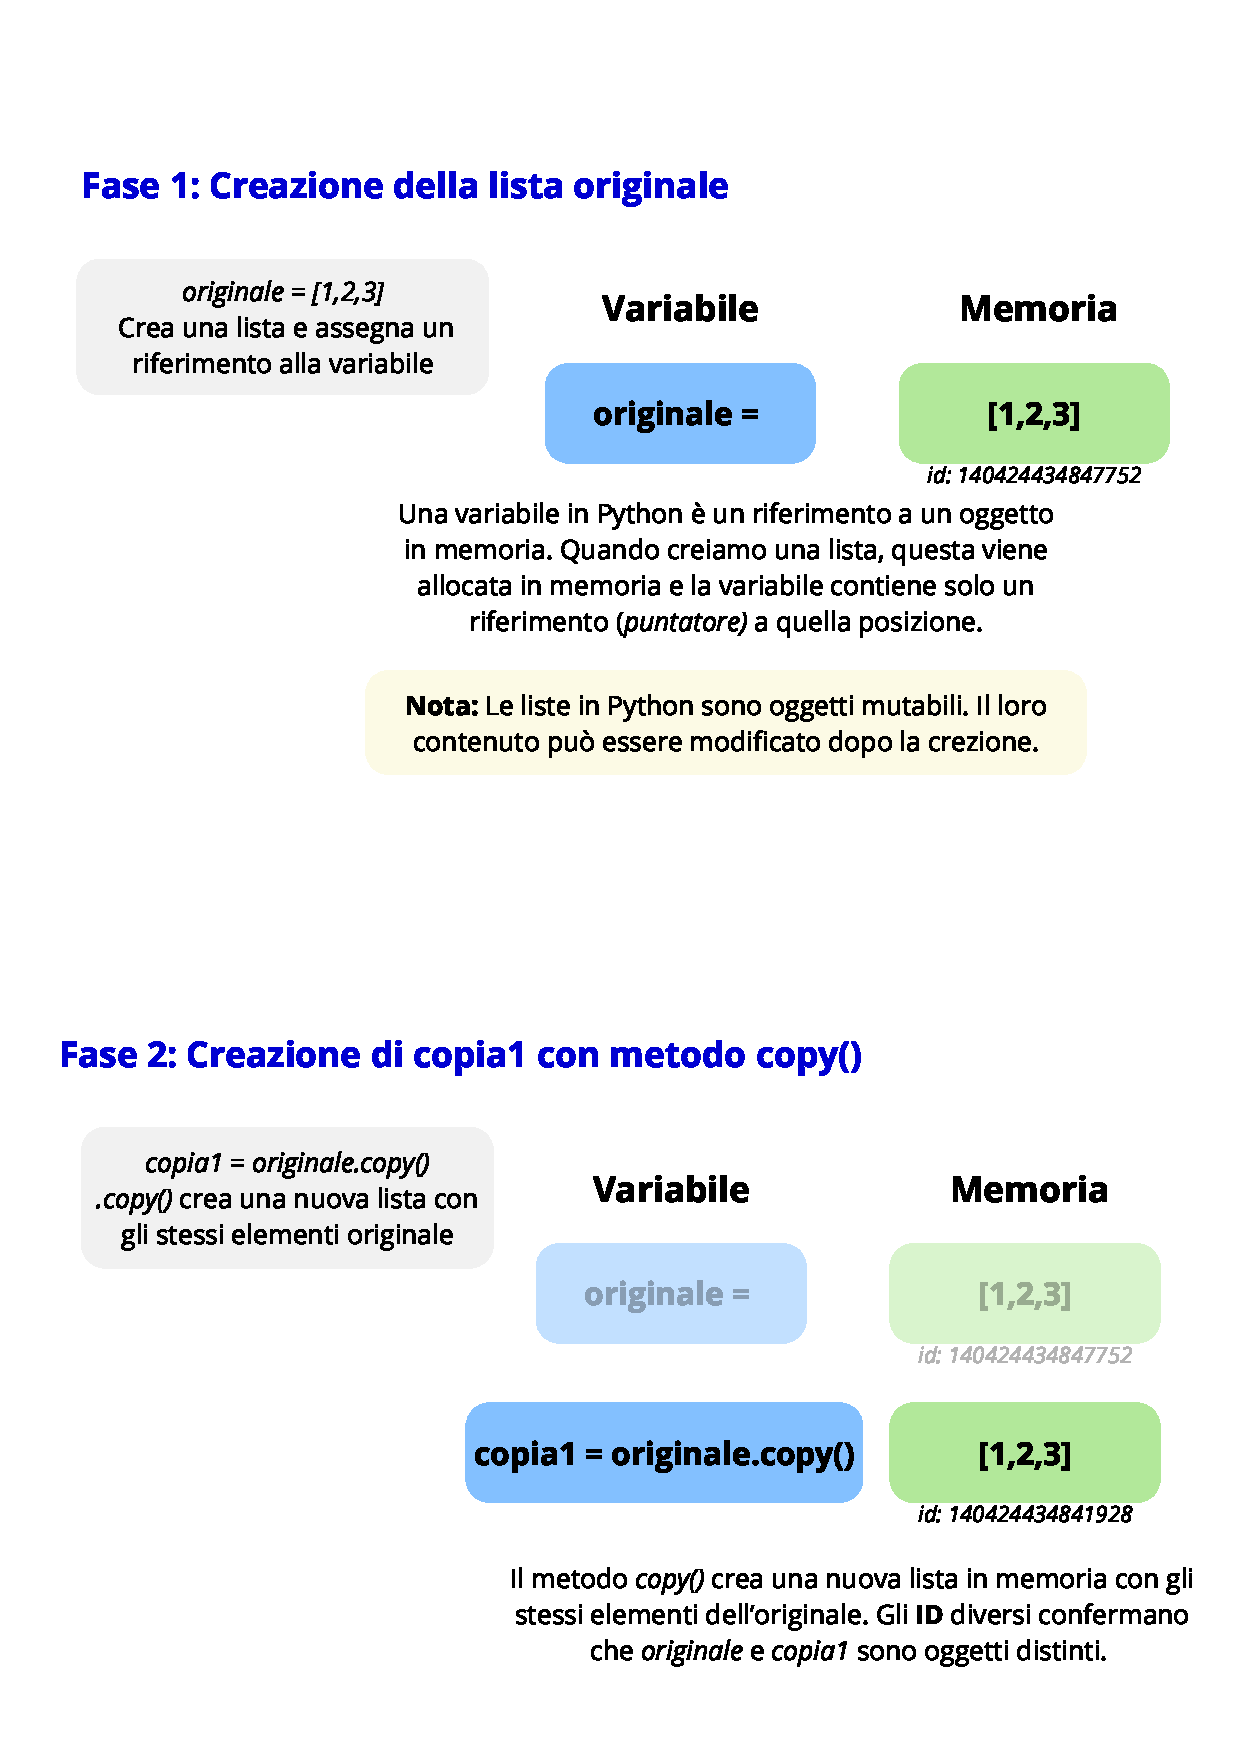
\includepdf[pages=-,scale=0.95,pagecommand={\thispagestyle{empty}},fitpaper=true]{pdf/Liste.pdf}

\paragraph{Il Problema delle Liste Annidate}\noindent

I metodi di copia visti sopra creano "copie superficiali" (shallow copies). Se la lista contiene altre liste (o oggetti mutabili), i metodi di copia standard copiano solo i riferimenti a queste liste interne, non le liste stesse. In pratica ogni modifica apportata alla lista originale, tramite \textit{shallow copies} influenzerà la sua copia.

Affrontiamo graficamente ciò che avviene con le liste annidate.

\begin{lstlisting}[language=Python]
# Lista con una lista annidata
originale = [1, 2, [3, 4]]

# Creazione di una copia superficiale
copia = originale.copy()

# Modifica della lista interna nell'originale
originale[2].append(5)

# La modifica si riflette anche nella copia!
print(originale)  # [1, 2, [3, 4, 5]]
print(copia)      # [1, 2, [3, 4, 5]]
\end{lstlisting}

\begin{center}
\begin{tikzpicture}
    % Definizione stili
    \tikzstyle{variable}=[draw, fill=blue!20, minimum width=2cm, minimum height=0.8cm, font=\bfseries]
    \tikzstyle{memory}=[draw, fill=green!20, minimum width=3.5cm, minimum height=1.2cm, rounded corners, font=\bfseries]
    \tikzstyle{innermemory}=[draw, fill=orange!20, minimum width=2.5cm, minimum height=1cm, rounded corners, font=\bfseries]
    \tikzstyle{reference}=[->, thick, blue]
    \tikzstyle{innerref}=[->, thick, orange]
    
    % Etichette per le sezioni
    \node[align=center, font=\bfseries] at (0,2.5) {Variabili};
    \node[align=center, font=\bfseries] at (4,2.5) {Liste Esterne};
    \node[align=center, font=\bfseries] at (8.5,2.5) {Lista Interna};
    
    % Variabili
    \node[variable = default] (var_orig) at (0,1) {originale};
    \node[variable = default] (var_copia) at (0,0) {copia};
    
    % Oggetti lista esterna in memoria
    \node[memory] (obj_orig) at (4,1.3) {[1, 2, riferimento]};
    \node[memory] (obj_copia) at (4,-0.1) {[1, 2, riferimento]};
    
    % Oggetto lista interna in memoria
    \node[innermemory] (obj_inner) at (8.5,0.5) {[3, 4, 5]};
    
    % Frecce di riferimento esterne
    \draw[reference] (var_orig) -- (obj_orig);
    \draw[reference] (var_copia) -- (obj_copia);
    
    % Frecce di riferimento interne
    \draw[innerref] (5.8,1) -- (obj_inner);
    \draw[innerref] (5.8,0) -- (obj_inner);
    
    % Spiegazione
    \node[text width=10cm, font=\small, align=center] at (4.2,-1.9) {
        Entrambe le liste esterne contengono riferimenti alla stessa lista interna.\\
        La modifica della lista interna è visibile attraverso entrambi i riferimenti.
    };
\end{tikzpicture}
\end{center}

\paragraph{Il Problema della Copia profonda in Dettaglio}

Come abbiamo accennato sopra \textit{"\nameref{metodiCopia}"}, sono metodi che creano una copia superficiale. Questo approccio presenta limitazioni significative quando si lavora con strutture di dati annidate:

\subparagraph{Comprensione del Problema}

Le copie superficiali duplicano solo la struttura esterna, mantendendo i riferimenti agli stessi oggetti interni.


% Fase 1: Confronto tra copia superficiale e copia profonda prima delle modifiche
\begin{figure}[htbp]
    \centering
    \begin{tikzpicture}[node distance=1.5cm]
        % Titolo
        \node[section title] at (0,2) {Fase 1: Confronto tra copia superficiale e copia profonda};
        
        % Etichette colonne
        \node[label] at (-4,1) {Variabile};
        \node[label] at (0,1) {Lista Esterna};
        \node[label] at (4,1) {Lista Interna};
        
        % Originale
        \node[variable={default}] (var_orig) at (-4,0) {originale};
        \node[memory] (mem_orig) at (0,0) {[1, 2, riferimento]};
        \node[memory] (mem_inner) at (4,0) {[3, 4]};
        \draw[reference] (var_orig) -- (mem_orig);
        \draw[reference] (mem_orig) -- (mem_inner);
        \node[id label] at (0,-0.8) {id: 140424434847752};
        \node[id label] at (4,-0.8) {id: 140424434830280};
        
        % Copia superficiale
        \node[variable={default}] (var_shallow) at (-4,-2) {copia\_superficiale};
        \node[memory] (mem_shallow) at (0,-2) {[1, 2, riferimento]};
        \draw[reference] (var_shallow) -- (mem_shallow);
        \draw[reference] (mem_shallow) to[out=0, in=190] (mem_inner);
        \node[id label] at (0,-2.8) {id: 140424434841928};
        
        % Copia profonda
        \node[variable={default}] (var_deep) at (-4,-4) {copia\_profonda};
        \node[memory] (mem_deep) at (0,-4) {[1, 2, riferimento]};
        \node[memory] (mem_inner_deep) at (4,-4) {[3, 4]};
        \draw[reference] (var_deep) -- (mem_deep);
        \draw[reference] (mem_deep) -- (mem_inner_deep);
        \node[id label] at (0,-4.8) {id: 140424434836104};
        \node[id label] at (4,-4.8) {id: 140424434825456};
        
        % Spiegazione
        \node[explanation] at (0,-6.5) {Confronto tra copie: la copia superficiale crea un nuovo oggetto 
        lista esterna ma mantiene il riferimento alla stessa lista interna dell'originale. 
        La copia profonda duplica sia la lista esterna che quella interna, creando oggetti completamente indipendenti.};
    \end{tikzpicture}
    \caption{Confronto tra copia superficiale e copia profonda prima della modifica}
    \label{fig:deep-copy-before}
\end{figure}

% Fase 2: Comportamento dopo la modifica
\begin{figure}[htbp]
    \centering
    \begin{tikzpicture}[node distance=1.5cm]
        % Titolo
        \node[section title] at (0,2) {Fase 2: Effetto delle modifiche sulla lista interna};
        
        % Etichette colonne
        \node[label] at (-4,1) {Variabile};
        \node[label] at (0,1) {Lista Esterna};
        \node[label] at (4,1) {Lista Interna};
        
        % Originale
        \node[variable={default}] (var_orig) at (-4,0) {originale};
        \node[memory] (mem_orig) at (0,0) {[1, 2, riferimento]};
        \node[memory] (mem_inner) at (4,0) {[3, 4, 5]};
        \draw[reference] (var_orig) -- (mem_orig);
        \draw[reference] (mem_orig) -- (mem_inner);
        \node[id label] at (0,-0.8) {id: 140424434847752};
        \node[id label] at (4,-0.8) {id: 140424434830280};
        
        % Copia superficiale
        \node[variable={default}] (var_shallow) at (-4,-2) {copia\_superficiale};
        \node[memory] (mem_shallow) at (0,-2) {[1, 2, riferimento]};
        \draw[reference] (var_shallow) -- (mem_shallow);
        \draw[reference] (mem_shallow) to[out=0, in=190] (mem_inner);
        \node[id label] at (0,-2.8) {id: 140424434841928};
        
        % Copia profonda
        \node[variable={default}] (var_deep) at (-4,-4) {copia\_profonda};
        \node[memory] (mem_deep) at (0,-4) {[1, 2, riferimento]};
        \node[memory] (mem_inner_deep) at (4,-4)  {[3, 4]};
        \draw[reference] (var_deep) -- (mem_deep);
        \draw[reference] (mem_deep) -- (mem_inner_deep);
        \node[id label] at (0,-4.8) {id: 140424434836104};
        \node[id label] at (4,-4.8) {id: 140424434825456};
        
        % Spiegazione
        \node[explanation] at (0,-6.5) {Dopo aver modificato la lista interna dell'originale con \texttt{originale[2].append(5)}, 
        la modifica si riflette anche nella copia superficiale perché entrambi condividono lo stesso oggetto interno. 
        La copia profonda rimane invariata perché contiene una duplicazione indipendente della lista interna.};
        
        % Evidenziazione della modifica
        \draw[red, thick, dashed] (4,0.04) circle (0.62);
        \node[red, font=\small\bfseries] at (3.2,-1.4) {Modificato};

        % Evidenziazione dell'effetto sulla copia superficiale  
        \draw[red, ->, thick, dashed] (6.5,-1) -- (5.1,-0.1);
        \node[red, text width=2.5cm, align=center, font=\small\bfseries] at (7.5,-1) {La modifica si riflette anche qui};
        
        % Evidenziazione dell'indipendenza della copia profonda
        \draw[green!60!black, ->, thick, dashed] (6.5,-4) -- (5.1,-4);
        \node[green!60!black, text width=2.5cm, align=center, font=\small\bfseries] at (7.5,-4) {Rimane invariata};
    \end{tikzpicture}
    \caption{Effetto delle modifiche: differenza tra copia superficiale e profonda}
    \label{fig:deep-copy-after}
\end{figure}

\newpage
\paragraph{Copie Profonde}

Per creare una "copia profonda" (deep copy) che copia anche gli oggetti annidati, si può utilizzare il modulo \texttt{copy}:

\begin{lstlisting}[language=Python]
import copy

# Lista con una lista annidata
originale = [1, 2, [3, 4]]

# Creazione di una copia profonda
copia_profonda = copy.deepcopy(originale)

# Modifica della lista interna nell'originale
originale[2].append(5)

# La copia profonda non è influenzata
print(originale)      # [1, 2, [3, 4, 5]]
print(copia_profonda) # [1, 2, [3, 4]]
\end{lstlisting}

\begin{center}
\begin{tikzpicture}
    % Definizione stili
    \tikzstyle{variable}=[draw, fill=blue!20, minimum width=2.5cm, minimum height=0.8cm, font=\bfseries]
    \tikzstyle{memory}=[draw, fill=green!20, minimum width=3.5cm, minimum height=1.2cm, rounded corners, font=\bfseries]
    \tikzstyle{innermemory}=[draw, fill=orange!20, minimum width=2.5cm, minimum height=1cm, rounded corners, font=\bfseries]
    \tikzstyle{reference}=[->, thick, blue]
    \tikzstyle{innerref}=[->, thick, orange]
    
    % Etichette per le sezioni
    \node[align=center, font=\bfseries] at (-0.5,2.5) {Variabili};
    \node[align=center, font=\bfseries] at (4,2.5) {Liste Esterne};
    \node[align=center, font=\bfseries] at (8.5,2.5) {Liste Interne};
    
    % Variabili
    \node[variable = default = default] (var_orig) at (-0.5,1) {originale};
    \node[variable = default] (var_copia) at (-0.5,0) {copia\_profonda};
    
    % Oggetti lista esterna in memoria
    \node[memory] (obj_orig) at (4,1.2) {[1, 2, riferimento]};
    \node[memory] (obj_copia) at (4,-0.2) {[1, 2, riferimento]};
    
    % Oggetti lista interna in memoria
    \node[innermemory] (obj_inner_orig) at (8.5,1) {[3, 4, 5]};
    \node[innermemory] (obj_inner_copia) at (8.5,0) {[3, 4]};
    
    % Frecce di riferimento esterne
    \draw[reference] (var_orig) -- (obj_orig);
    \draw[reference] (var_copia) -- (obj_copia);
    
    % Frecce di riferimento interne
    \draw[innerref] (5.8,1) -- (obj_inner_orig);
    \draw[innerref] (5.8,0) -- (obj_inner_copia);
    
    % Spiegazione
    \node[text width=10cm, font=\small, align=center] at (4,-1.7) {
        Con una copia profonda, sia la lista esterna che quelle interne vengono copiate.\\
        Le modifiche alla lista interna dell'originale non influenzano la copia.
    };
\end{tikzpicture}
\end{center}


\subsubsection{Confronto tra Liste: `==` vs `is`}\label{ConfrontoOperatoriListe}

Python fornisce due modi per confrontare le liste:
\begin{itemize}
    \item L'operatore \texttt{==} confronta il contenuto delle liste (uguaglianza di valore)
    \item L'operatore \texttt{is} confronta gli identificatori degli oggetti (uguaglianza di identità)
\end{itemize}

\begin{lstlisting}[language=Python]
a = [1, 2, 3]
b = [1, 2, 3]  # Una nuova lista con gli stessi valori
c = a          # Riferimento alla stessa lista

print(a == b)  # True - stesso contenuto
print(a is b)  # False - oggetti diversi in memoria
print(a is c)  # True - stesso oggetto in memoria
\end{lstlisting}

\subsubsection{Rappresentazione Visiva della Memoria}



\begin{lstlisting}[language=Python]
a = [1, 2, 3]
b = [1, 2, 3]  # Una nuova lista con gli stessi valori
c = a          # Riferimento alla stessa lista

print(a == b)  # True - stesso contenuto
print(a is b)  # False - oggetti diversi in memoria
print(a is c)  # True - stesso oggetto in memoria

# Visualizzazione degli id per conferma
print(id(a))  # Ad esempio: 140424434847752
print(id(b))  # Diverso da a
print(id(c))  # Stesso di a
\end{lstlisting}

\begin{center}
\begin{tikzpicture}
    % Definizione stili
    \tikzstyle{variable}=[draw, fill=blue!20, minimum width=2cm, minimum height=0.8cm, font=\bfseries]
    \tikzstyle{memory}=[draw, fill=green!20, minimum width=3cm, minimum height=1.2cm, rounded corners, font=\bfseries]
    \tikzstyle{reference}=[->, thick, blue]
    
    % Etichette per le sezioni
    \node[align=center, font=\bfseries] at (0,3) {Variabili};
    \node[align=center, font=\bfseries] at (4.5,3) {Oggetti in Memoria};
    
    % Variabili
    \node[variable = default] (var_a) at (0,2) {a};
    \node[variable = default] (var_b) at (0,0.5) {b};
    \node[variable = default] (var_c) at (0,-1) {c};
    
    % Oggetti in memoria
    \node[memory] (obj_a) at (4.5,2) {[1, 2, 3]};
    \node[memory] (obj_b) at (4.5,0.5) {[1, 2, 3]};
    
    % IDs
    \node[right, font=\small] at (obj_a.east) {id: 140424434847752};
    \node[right, font=\small] at (obj_b.east) {id: 140424434841928};
    
    % Frecce di riferimento
    \draw[reference] (var_a) -- (obj_a);
    \draw[reference] (var_b) -- (obj_b);
    \draw[reference] (var_c) to [out=0, in=180] (obj_a);
    
    % Spiegazione
    \node[text width=8cm, font=\small, align=center] at (2.2,-2.5) {
        \texttt{a == b} è \texttt{True} (stesso contenuto)\\
        \texttt{a is b} è \texttt{False} (oggetti diversi)\\
        \texttt{a is c} è \texttt{True} (stesso oggetto)
    };
\end{tikzpicture}
\end{center}

\paragraph{Errore Comune: Liste Annidate Moltiplicate}

Un errore comune quando si lavora con liste annidate è la creazione di matrici usando la moltiplicazione di liste:

\begin{lstlisting}[language=Python]
# Tentativo ERRATO di creare una matrice 3x3 di zeri
matrice_errata = [[0] * 3] * 3
print(matrice_errata)  # [[0, 0, 0], [0, 0, 0], [0, 0, 0]]

# Modifica di un solo elemento
matrice_errata[0][0] = 1
print(matrice_errata)  # [[1, 0, 0], [1, 0, 0], [1, 0, 0]]  Oops!
\end{lstlisting}

Cosa è successo? L'espressione `[[0] * 3] * 3` crea una lista contenente tre riferimenti alla stessa lista interna. Quando modifichi un elemento in una "riga", la modifica appare in tutte le righe perché puntano allo stesso oggetto.

\begin{center}
\begin{tikzpicture}
    % Definizione stili
    \tikzstyle{variable}=[draw, fill=blue!20, minimum width=2cm, minimum height=0.8cm, font=\bfseries]
    \tikzstyle{memory}=[draw, fill=green!20, minimum width=3.5cm, minimum height=1.2cm, rounded corners, font=\bfseries]
    \tikzstyle{innermemory}=[draw, fill=orange!20, minimum width=2.5cm, minimum height=1cm, rounded corners, font=\bfseries]
    \tikzstyle{reference}=[->, thick, blue]
    \tikzstyle{innerref}=[->, thick, orange]
    
    % Variabile
    \node[variable = default] (var_matrice) at (0,0) {matrice\_errata};
    
    % Oggetto lista esterna in memoria
    \node[memory] (obj_matrice) at (4,0) {[rif, rif, rif]};
    
    % Oggetto lista interna in memoria (una sola lista per tutte e 3 le righe!)
    \node[innermemory] (obj_inner) at (8,0) {[1, 0, 0]};
    
    % Frecce di riferimento esterne
    \draw[reference] (var_matrice) -- (obj_matrice);
    
    % Frecce di riferimento interne - tutte puntano alla stessa lista interna!
    \draw[innerref] (5.2,0.2) -- (obj_inner);
    \draw[innerref] (5.2,0) -- (obj_inner);
    \draw[innerref] (5.2,-0.2) -- (obj_inner);
\end{tikzpicture}
\end{center}

\paragraph{Soluzione Corretta}

Il modo corretto per creare liste annidate indipendenti è utilizzare una comprensione di lista:

\begin{lstlisting}[language=Python]
# Modo CORRETTO:
matrice_corretta = [[0 for _ in range(3)] for _ in range(3)]
matrice_corretta[0][0] = 1
print(matrice_corretta)  # [[1, 0, 0], [0, 0, 0], [0, 0, 0]]
\end{lstlisting}

\begin{center}
\begin{tikzpicture}
    % Definizione stili
    \tikzstyle{variable}=[draw, fill=blue!20, minimum width=2.5cm, minimum height=0.8cm, font=\bfseries]
    \tikzstyle{memory}=[draw, fill=green!20, minimum width=3.5cm, minimum height=1.2cm, rounded corners, font=\bfseries]
    \tikzstyle{innermemory}=[draw, fill=orange!20, minimum width=2.5cm, minimum height=1cm, rounded corners, font=\bfseries]
    \tikzstyle{reference}=[->, thick, blue]
    \tikzstyle{innerref}=[->, thick, orange]
    
    % Variabile
    \node[variable = default] (var_matrice) at (0,0) {matrice\_corretta};
    
    % Oggetto lista esterna in memoria
    \node[memory] (obj_matrice) at (4,0) {[rif, rif, rif]};
    
    % Oggetti lista interna in memoria (tre liste diverse!)
    \node[innermemory] (row1) at (8,1) {[1, 0, 0]};
    \node[innermemory] (row2) at (8,0) {[0, 0, 0]};
    \node[innermemory] (row3) at (8,-1) {[0, 0, 0]};
    
    % Frecce di riferimento esterne
    \draw[reference] (var_matrice) -- (obj_matrice);
    
    % Frecce di riferimento interne - ciascuna punta a una lista diversa
    \draw[innerref] (5.8,0.2) -- (row1);
    \draw[innerref] (5.8,0) -- (row2);
    \draw[innerref] (5.8,-0.2) -- (row3);
\end{tikzpicture}
\end{center}

In questo caso, ogni riga è un oggetto lista separato e indipendente. Modificando un elemento in una riga, le altre righe non sono influenzate.

\paragraph{Implicazioni Pratiche}

Comprendere come funzionano i riferimenti in Python ha importanti implicazioni pratiche:

\begin{itemize}
    \item \textbf{Modifiche indesiderate}: Modificare una lista attraverso un riferimento influenza tutti i riferimenti alla stessa lista
    \item \textbf{Copie superficiali non sufficienti}: Quando la lista contiene oggetti mutabili, una copia superficiale potrebbe non essere sufficiente
    \item \textbf{Confronto con \texttt{is}}: Utilizzare \texttt{is} quando si intende confrontare il contenuto può portare a risultati inaspettati
\end{itemize}
\begin{center}

\end{center}

\subsubsection{Implicazioni Pratiche}

Comprendere come funzionano i riferimenti in Python ha importanti implicazioni pratiche:

\begin{tcolorbox}[colback=red!5!white,colframe=red!75!black,title=Errori comuni con i riferimenti alle liste]
\begin{itemize}
    \item \textbf{Modifiche indesiderate}: Modificare una lista attraverso un riferimento influenza tutti i riferimenti alla stessa lista
    \item \textbf{Copie superficiali non sufficienti}: Quando la lista contiene oggetti mutabili, una copia superficiale potrebbe non essere sufficiente
    \item \textbf{Confronto con \texttt{is}}: Utilizzare \texttt{is} quando si intende confrontare il contenuto può portare a risultati inaspettati
\end{itemize}
\end{tcolorbox}

%Sezione per Esercizi Sulle Liste
\clearpage

\subsection{Esercizi Riassuntivi}
Come per la sezione sulle \textit{\hyperref[EserciziFondamenti]{variabili}}, anche qui andiamo a svolgere alcuni esercizi per familiarizzare con i concetti affrontati, anche qui a fine sezione si troveranno gli esercizi svolti con le soluzioni spiegate passo passo.

\subsubsection{Esercizio 1: Concetti Base e Indicizzazione}\label{Esercizio1Liste}
In questo esercizio andremo ad approfondire il concetto di indicizzazione, vedi capitolo \nameref{IndicizzazioneListe}
    \newline
\textbf{Traccia gli Indici:} Data la lista \textit{colori = ["rosso", "verde", "blu", "giallo", "viola"]}

-   Scrivi l'indice positivo e negativo per accedere a ciascun elemento

-   Qual è il valore di colori[1]? E di colori[-2]

-   Se volessi accedere a \textit{"verde"} usando un indice negativo, quale sarebbe?

\vspace{0,5cm}
\begin{lstlisting}
#Dichiariamo la lista colori
colori = ["rosso", "verde", "blu", "giallo", "viola"]

#Inserisci gli indici positivi e negativi di tutti gli elementi della lista

#Valore di colori[1]

#Valore di colori[-2]

#A quale indice corrisponde "verde" e quale sarebbe il suo corrispettivo indice negativo?

\end{lstlisting}

\subsubsection{Esercizio 2: Operazioni Base sulle Liste}\label{Esercizio2Liste}
\title{\textbf{Modifica gli Elementi}}
inizializziamo una lista punteggi.

\begin{lstlisting}
punteggi = [85, 92, 78, 90, 88]
# - Sostituisci il terzo elemento con 95

# - Aggiungi 100 alla fine della lista

# - Inserisci 82 nella seconda posizione

\end{lstlisting}

\title{\textbf{Concatenazione e Ripetizione}}
\begin{lstlisting}
# Scrivi il risultato di queste operazioni:

lista1 = [1, 2, 3]
lista2 = [4, 5]
risultato1 = lista1 + lista2
risultato2 = lista1 * 3
\end{lstlisting}

Per questo esercizio, ripassare le sezioni:
\begin{itemize}
    \item \nameref{MetodiListe}
    \item \nameref{MetodiListeRemove}
\end{itemize}



\subsubsection{Esercizio 3: Slicing delle Liste}\label{Esercizio3Liste}
\title{\textbf{Estrazioni con Slicing}}

\begin{lstlisting}
# Data una lista
lettere = ["a", "b", "c", "d", "e", "f", "g"]

# - Estrarre i primi due elementi

# - Estrai gli ultimi due elementi

# - Estrai gli elementi dallaa posizione 2 alla 5 (inclusa)

# - Estrai tutti gli elementi tranne il primo e l'ultimo
\end{lstlisting}

\title{\textbf{Slicing Avanzato}}
\begin{lstlisting}
# Prevedi il risultato di questo codice:

sequenza = [10, 20, 30, 40, 50, 60, 70]
parte1 = sequenza[1:5]
parte2 = sequenza[::2]
parte3 = sequenza[5:1:-1]
\end{lstlisting}


Per questo esercizio, ripassare le sezioni:
\begin{itemize}
    \item \nameref{SlicingListe}
\end{itemize}

\subsubsection{Esercizio 4: Metodi delle Liste}\label{Esercizio4Liste}
\title{\textbf{Applicazione dei metodi base}}

\begin{lstlisting}
# Data una lista
frutta = ["mela", "banana", "ciliegia"]

# - Usa il metodo appropriato per aggiungere "arancia" alla fine
    
# - Usa il metodo corretto per trovare la posizione di "banana"

# - Usa un metodo per contare quante volte appare "mela"

# - Usa un metodo per rimuovere "ciliegia"

\end{lstlisting}


\title{\textbf{Ordinamento e Inversione:}}


\begin{lstlisting}
# Data una lista di numeri
numeri = [42, 8, 16, 23, 4, 15]

# - Ordina la lista in modo crescente

# - Inverti l'ordine degli elementi

# - Qual è la differenza tra usare il metodo sort() e la funzione sorted()
\end{lstlisting}






Per questo esercizio ripassare le sezioni:
\begin{itemize}
    \item \nameref{MetodiOrdinamentoInversioneListe}
    \item \nameref{EsempiInputCountListe}
    \item  \nameref{AccessoListe}
    \item  \nameref{MetodiInfoListe}
\end{itemize}


\subsubsection{Esercizio 5: Comportamento in Memoria delle Liste}\label{Esercizio5Liste}
\title{\textbf{Riferimenti e Copie}}


\begin{lstlisting}
# Analizza e predici l'Output

a = [1, 2, 3]
b = a
b[0] = 10
print(a)

\end{lstlisting}


\title{\textbf{Creazione di Copie Indipendenti:}}
\begin{lstlisting}
# Quali tra questi metodi creanno una copia indipendente?

lista2 = lista1

lista2 = lista1[:]

lista2 = list(lista1)

lista2 = lista1.copy()

\end{lstlisting}


\title{\textbf{Identità vs Uguaglianza:}}
\begin{lstlisting}
# Predici il risultato di questi confronti:

lista1 = [1, 2, 3]
lista2 = [1, 2, 3]
lista3 = lista1

print(lista1 == lista2)
print(lista1 is lista2)
print(lista1 is lista3)

\end{lstlisting}



Per questo esercizio ripassare le sezioni:
\begin{itemize}
    \item \nameref{ComportamentoInMemoriaListe}
\end{itemize}

\subsubsection{Esercizio 6: Analisi di Codice e Risoluzione Problemi:}\label{Esercizio6Liste}
\title{\textbf{Trova l'errore}}


\begin{lstlisting}
# Indentifica e correggi l'errore in questo codice:

colori = ["rosso", "verde", "blu"]
colori[3] = "giallo"  # Aggiungi giallo alla lista
print(colori[4])      # Stampa il quinto elemento

\end{lstlisting}


\title{\textbf{Tracciamento della Memoria:}}
\begin{lstlisting}
# Dissegna un diagramma di memoria che mostri lo stato delle varaibili dopo ogni istruzione

lista1 = [10, 20]
lista2 = lista1
lista1.append(30)
lista3 = lista1[:]
lista3[0] = 99

\end{lstlisting}


\title{\textbf{Test di Comprensione}}
\begin{lstlisting}
# Cosa Stampa questo codice

a = [1, 2, 3]
b = [a, a]
b[0][1] = 10
print(b)
print(a)

\end{lstlisting}



Per questo esercizio ripassare le sezioni:
\begin{itemize}
    \item \nameref{ComportamentoInMemoriaListe}
\end{itemize}


\subsection{Risoluzione Esercizi Sulle Liste}

\subsubsection{Risoluzione Esercizio 1: \nameref{Esercizio1Liste}}

\begin{lstlisting}
# Data la lista colori = ["rosso", "verde", "blu", "giallo", "viola"]

#Inserisci gli indici positivi e negativi di tutti gli elementi della lista
    #Per risolvere questo quesito potremmo prima vedere quanto è lunga la lista
    print(len(colori))
    
    #In questo modo conosceremo quanti elementi sono presenti nella lista e potremo numerarli in entrambi i versi

    # Formula: indice_negativo = -lunghezza + indice_positivo
    
    # "rosso": indice positivo 0, indice negativo = -5 + 0 = -5
    # "verde": indice positivo 1, indice negativo = -5 + 1 = -4
    # "blu": indice positivo 2, indice negativo = -5 + 2 = -3
    # "giallo": indice positivo 3, indice negativo = -5 + 3 = -2
    # "viola": indice positivo 4, indice negativo = -5 + 4 = -1
        
#Valore di colori[1]
    #Dopo aver numerato gli elementi della lista ora possiamo ricavare i valori all'indice richiesto
#    - Verde
#Valore di colori[-2]
#    - Giallo
#A quale indice corrisponde "verde" e quale sarebbe il suo corrispettivo indice negativo?
#Ricaviamolo dalla numerazione svolta prima
#"verde"  - lunghezza 5 + indice positivo 1 = 1 -5 = -4
\end{lstlisting}


\subsubsection{Risoluzioe Esercizio 2: \nameref{Esercizio2Liste}}

\begin{lstlisting}
punteggi = [85, 92, 78, 90, 88]
# - Sostituisci il terzo elemento con 95

    # Prima di sostituire il numero troviamolo, stampiamo la lunghezza della lista cosi da facilitare la numerazione degli elementi.
    print(len(punteggi))
    # Ora numeramio gli elementi
    # b = 80 (30 + 50 = 80, il terzo elemento più l'ultimo)
    # a = 10 (il primo elemento)
    # c = 30 (il terzo elemento dalla fine)

# Ora possiamo sostituire il terzo elemento con 95
    punteggi[2] = 95
    
# - Aggiungi 100 alla fine della lista
    # Qui possiamo agire in diversi modi: 
    
    #Concatenazione con una lista contenente il nuovo elemento:
        punteggi = punteggi + [100]
    
    #Operatore di aggiunta in-place:
        punteggi += [100]
    
    #Metodo extend con una lista singola:
        punteggi.extend([100])
    
    #Slice assignment alla fine della lista:
        punteggi[len(punteggi):] = [100]
    
    #Insert all'indice finale:
        punteggi.insert(len(punteggi), 100)
    
    # - Inserisci 82 nella seconda posizione


# === SECONDA PARTE ===

# Scrivi il risultato di queste operazioni:

lista1 = [1, 2, 3]
lista2 = [4, 5]
risultato1 = lista1 + lista2
risultato2 = lista1 * 3

    # risultato1 = [1, 2, 3, 4, 5] (concatenazione delle due liste)
    # risultato2 = [1, 2, 3, 1, 2, 3, 1, 2, 3] (ripetizione della prima lista 3 volte)
\end{lstlisting}


\subsubsection{Risoluzione Esercizio 3: \nameref{Esercizio3Liste}}

\begin{lstlisting}
# Data una lista
lettere = ["a", "b", "c", "d", "e", "f", "g"]

# Primi tre elementi
primi_tre = lettere[:3]  # ["a", "b", "c"]

# Ultimi due elementi
ultimi_due = lettere[-2:]  # ["f", "g"]

# Elementi dalla posizione 2 alla 5 (inclusa)
dalla_2_alla_5 = lettere[2:6]  # ["c", "d", "e", "f"]

# Tutti tranne primo e ultimo
senza_primo_ultimo = lettere[1:-1]  # ["b", "c", "d", "e", "f"]

# === SECONDA PARTE ===

Prevedi il risultato di questo codice:

sequenza = [10, 20, 30, 40, 50, 60, 70]
parte1 = sequenza[1:5]
parte2 = sequenza[::2]
parte3 = sequenza[5:1:-1]

#parte1 = [20, 30, 40, 50] (elementi dall'indice 1 all'indice 4 incluso)
#parte2 = [10, 30, 50, 70] (ogni elemento a passo 2, partendo dall'inizio)
#parte3 = [60, 50, 40, 30] (dall'indice 5 all'indice 2 incluso, in ordine inverso)
\end{lstlisting}

\subsubsection{Risoluzione Esercizio 4: \nameref{Esercizio4Liste}}

\begin{lstlisting}
# Data una lista
frutta = ["mela", "banana", "ciliegia"]

# - Usa il metodo appropriato per aggiungere "arancia" alla fine
    frutta.append("arancia")
    print(frutta)  # ["mela", "banana", "ciliegia", "arancia"]
    
# - Usa il metodo corretto per trovare la posizione di "banana"
    posizione_banana = frutta.index("banana")  # 1
    
# - Usa un metodo per contare quante volte appare "mela"
    occorrenze_mela = frutta.count("mela")  # 1
    
# - Usa un metodo per rimuovere "ciliegia"
    frutta.remove("ciliegia")
    print(frutta)  # ["mela", "banana", "arancia"]


# === SECONDA PARTE ===


# Data una lista di numeri
numeri = [42, 8, 16, 23, 4, 15]

# - Ordina la lista in modo crescente
    numeri.sort()
    print(numeri)  # [4, 8, 15, 16, 23, 42]
    
# - Inverti l'ordine degli elementi
    numeri.reverse()
    print(numeri)  # [42, 23, 16, 15, 8, 4]
    
# - Qual è la differenza tra usare il metodo sort() e la funzione sorted()
    # Differenza tra sort() e sorted():
    # - sort() modifica la lista originale
    # - sorted() crea una nuova lista ordinata lasciando l'originale intatta

originale = [3, 1, 2]
nuova = sorted(originale)
print(originale)  # [3, 1, 2] rimane invariata
print(nuova)      # [1, 2, 3] nuova lista ordinata
\end{lstlisting}


\subsubsection{Risoluzione Esercizio 5: \nameref{Esercizio5Liste}}

\begin{lstlisting}
# Analizza e predici l'Output

a = [1, 2, 3]
b = a
b[0] = 10
print(a)

    # Soluzione: L'output sarà [10, 2, 3] 
    # Spiegazione: b è un riferimento alla stessa lista di a. Modificando b, si  # modifica anche a perchè entrambe le variabili puntano allo stesso oggetto # in memoria.


# === SECONDA PARTTE ===


# Predici il risultato di questi confronti:

lista1 = [1, 2, 3]
lista2 = [1, 2, 3]
lista3 = lista1

print(lista1 == lista2)
print(lista1 is lista2)
print(lista1 is lista3)

# lista1 == lista2  -> True (confronta i contenui che sono uguali)
# lista1 is lista2 -> False (si riferiscono a oggetti diversi in memoria)
# lista1 is lista3  -> True (si riferiscono allo stesso oggetto in memoria)


lista1 == lista2 
#True (confronta i contenuti, che sono uguali)
lista1 is lista2 
#False (si riferiscono a oggetti diversi in memoria)
lista1 is lista3 
#True (si riferiscono allo stesso oggetto in memoria)
\end{lstlisting}


\subsubsection{Risoluzione Esercizio 6: \nameref{Esercizio6Liste}}

\begin{lstlisting}
# Indentifica e correggi l'errore in questo codice:

colori = ["rosso", "verde", "blu"]
colori[3] = "giallo"  # Aggiungi giallo alla lista
print(colori[4])      # Stampa il quinto elemento

#Non si puo usare colori[3] = "giallo" perchè l'indice 3 è fuori dal range (la #lista ha indici 0, 1, 2).
#Anche dopo aver aggiunto "giallo", colori[4] sarebbe fuori range.

# Correzione:
colori = ["rosso", "verde", "blu"]
colori.append("giallo")  # Corretto: aggiunge "giallo" alla fine
print(colori[3])         # Corretto: stampa il quarto elemento (giallo)



# === SECONDA PARTE === 

# Dissegna un diagramma di memoria che mostri lo stato delle varaibili dopo ogni istruzione


lista1 = [10, 20]
lista2 = lista1
lista1.append(30)
lista3 = lista1[:]
lista3[0] = 99


#lista1 = [10, 20]:

#lista1 -> [10, 20]


lista2 = lista1:

#lista1 -> [10, 20]
#lista2 -> [10, 20] (stesso oggetto di lista1)


lista1.append(30):

#lista1 -> [10, 20, 30]
#lista2 -> [10, 20, 30] (stesso oggetto di lista1)


lista3 = lista1[:]:

#lista1 -> [10, 20, 30]
#lista2 -> [10, 20, 30] (stesso oggetto di lista1)
#lista3 -> [10, 20, 30] (nuovo oggetto, copia di lista1)


lista3[0] = 99:

#lista1 -> [10, 20, 30]
#lista2 -> [10, 20, 30] (stesso oggetto di lista1)
#lista3 -> [99, 20, 30]


# === TERZA PARTE ===

# Cosa stampa questo codice
a = [1, 2, 3]
b = [a, a]
b[0][1] = 10
print(b)
print(a)


print(b): [[1, 10, 3], [1, 10, 3]]
print(a): [1, 10, 3]

#Spiegazione:

#a è una lista [1, 2, 3]
#b è una lista che contiene due riferimenti alla stessa lista a: [[1, 2, 3], [1, #2, 3]]
#b[0][1] = 10 modifica il secondo elemento della prima sottolista di b (che è #a), #quindi ora a è [1, 10, 3]
#Poichè entrambi gli elementi di b sono riferimenti alla stessa lista a, la #modifica si riflette in entrambiprint(b): [[1, 10, 3], [1, 10, 3]]
#print(a): [1, 10, 3]
\end{lstlisting}

\newpage
%Sezione III.2 TUPLE
\subsection{Tuple}\label{Tuple}

In questo capitolo andremo ad esplorare cosa sono e come usare le \textit{Tuple} in Python.

\vspace{0,5cm}


In Python una \textbf{tupla} è una collezione ordinata e \hyperref[mutableImmutable]{\textbf{immutabile}} di elementi. Questo significa che una volta creata una tupla, non è possibile modificarne il contenuto (aggiungere, rimuovere o cambiare elementi). 

Le tuple sono simili alle liste, ma con questa fondamentale differenza di immutabilità. Vengono spesso utilizzate per rappresentare collezioni di elementi eterogenei che non dovrebbero cambiare, come ad esempio le coordinate di un punto (x,y) o i record di un database.

Anche in questo capitolo andremo ad affrontare i vari casi d'uso, trattandoli successivamente in ambiti più avanzati.

\subsubsection{Caratteristiche Principali delle Tuple}\label{CaratteristicheTuple}

Analizziamo le caratteristiche principali delle tuple, come già accennato sopra, le tuple sono oggetti immutabili che non possono essere modificate, ma condividono molte caratteristiche con le  \hyperref[ListeCap1]{liste.}

\begin{tcolorbox}[colback=blue!5!white,colframe=blue!75!black,title=Caratteristiche principali delle Tuple]
\begin{itemize}
    \item \textbf{Delimitate da parentesi tonde}: Le tuple si creano racchiudendo gli elementi tra parentesi tonde ()
    \item \textbf{Ordinate}: Gli elementi mantengono l'ordine in cui sono stati inseriti
    \item \textbf{Immutabili}: Non è possibile modificare, aggiungere o rimuovere elementi dopo la creazione
    \item \textbf{Indicizzate}: Si può accedere agli elementi tramite indici numerici, partendo da 0, come nelle liste
    \item \textbf{Eterogenee}: Possono contenere elementi di tipi diversi (numeri, stringhe, booleani, altre liste, ecc.)
    \item \textbf{Duplicati ammessi}: Possono contenere elementi ripetuti
\end{itemize}
\end{tcolorbox}


\subsubsection{Sintassi Base delle Tuple}\label{SintassiTuple}

Come si inizializzano le tuple?

In Python esistono diversi modi per creare una tupla, Esaminiamo i più comuni.



\begin{lstlisting}[language=Python]
# Utilizzando le parentesi tonde ():
    # questo è il metodo più comune, gli elementi devono essere separati da virgole.
mia_tupla = (1,2,3,"a",True,2.3)
coordinate = (19.3,20.5)

# Senza le parentesi tonde () Usando il Tuple Packing, è possibile creare una tupla omettendo le parentesi, assegnando una sequenza di valori separati da virgola, in questo modo Python interpreterà automaticamente come tuple.

packing_Tuple = 1,23,"hello"  # Equivalente a packing_Tuple = (1,23,"hello")

# Come per le liste anche per le tuple esiste il suo costruttore:  tuple(), ma ha una sintassi leggermente diversa.

tupla_da_lista = tuple([1,2,3])

# Quando eseguiamo il costruttore su una stringa trasforma la stringa in un oggetto iterabile, del tutto simile a ciò che avviene con le liste.

tupla_da_stringa = tuple("python") # Risultato: ('p', 'y', 't', 'h', 'o', 'n')


# Per presentare una tupla con un singolo elemento è necessario includere una virgola finale dopo l'elemento. Altrimenti Python interpreterà l'espressione come il tipo dell'elemento stesso racchiuso tra parentesi (ad esempio, un intero, una stringa)

tupla_singola = (5,)
non_tupla = (5)  # Questo per python è un intero

\end{lstlisting}

\subsubsection{Operazioni comuni con le Tuple}\label{OperationBaseTuple}

Anche se immutabili le tuple supportano diverse operazioni che non modificano la tupla originale, ma ne creano di nuove o ne estraggono informazioni.

\subsubsection{{Acccesso agli elementi (indicizzazione):}}\label{TupleIndicizzazione}

Come per le liste, l'indicizzazione per le tuple è identica; pertanto, si può ripassare il capitolo in merito: \hyperref[IndicizzazioneListe]{\textit{{\textbf{Capitolo Indicizzazione.}}}}


\vspace{0,5cm}
\begin{lstlisting}
tupla = (10, 20, 30, 40, 50)

# Accesso tramite indice positivo (da sinistra)
primo_elemento = tupla[0]  # 10

# Accesso tramite indice negativo (da destra)
ultimo_elemento = tupla[-1]  # 50

# Slicing: estrazione di sottotuple
sottotupla = tupla[1:4]  # (20, 30, 40)
\end{lstlisting}



\vspace{0,5cm}

\subsubsection{{Slicing:}}\label{SlicingTuple}

Anche qui, come per le liste, è possibile effettuare lo slicing, anche per ottenere una sotto-tupla. Le modalità dello slicing sono le stesse; pertanto, è possibile fare riferimento al capitolo dedicato nelle liste: \hyperref[SlicingListe]{\textit{\textbf{Capitolo dedicato allo Slicing.}}}

\begin{lstlisting}
mia_tupla[inizio:fine:passo]

# Elementi dall'indice 2 all'indice 5 (escluso)
sotto_tupla1 = numeri[2:5]
print(sotto_tupla1)  # Output: (2, 3, 4)

# Elementi dall'inizio fino all'indice 4 (escluso)
sotto_tupla2 = numeri[:4]
print(sotto_tupla2)  # Output: (0, 1, 2, 3)

# Elementi dall'indice 6 fino alla fine
sotto_tupla3 = numeri[6:]
print(sotto_tupla3)  # Output: (6, 7, 8, 9)

# Tutti gli elementi (crea una copia)
sotto_tupla4 = numeri[:]
print(sotto_tupla4)  # Output: (0, 1, 2, 3, 4, 5, 6, 7, 8, 9)


# === Esempi usando Indici Negativi ===

# Ultimi 3 elementi
sotto_tupla5 = numeri[-3:]
print(sotto_tupla5)  # Output: (7, 8, 9)

# Dal terzo all'ultimo fino al penultimo
sotto_tupla6 = numeri[-3:-1]
print(sotto_tupla6)  # Output: (7, 8)

# Dal quarto elemento fino al terz'ultimo
sotto_tupla7 = numeri[3:-3]
print(sotto_tupla7)  # Output: (3, 4, 5, 6)


# === Slicing con Passo, Step ===

# Ogni secondo elemento dall'inizio alla fine
sotto_tupla8 = numeri[::2]
print(sotto_tupla8)  # Output: (0, 2, 4, 6, 8)

# Ogni terzo elemento dall'indice 1 all'indice 8
sotto_tupla9 = numeri[1:8:3]
print(sotto_tupla9)  # Output: (1, 4, 7)

# Passo negativo: inversione della tupla
sotto_tupla10 = numeri[::-1]
print(sotto_tupla10)  # Output: (9, 8, 7, 6, 5, 4, 3, 2, 1, 0)

# Elementi pari in ordine inverso
sotto_tupla11 = numeri[::-2]
print(sotto_tupla11)  # Output: (9, 7, 5, 3, 1)
\end{lstlisting}

\vspace{0,5cm}

\subsubsection{{Concatenazione delle Tuple}}\label{ConcatenazioneTuple}

In Python è possibile effettuare la concatenazione delle tuple, verosimilmente a ciò che avviene con le liste.


\begin{lstlisting}
    # Concatenazione di tuple
tupla1 = (1, 2, 3)
tupla2 = (4, 5, 6)
tupla_combinata = tupla1 + tupla2

print(tupla_combinata)  # Output: (1, 2, 3, 4, 5, 6)
\end{lstlisting}

\paragraph{Aspetti Teorici:}
Principi Fondamentali per la \textit{Concatenazione} delle Tuple.
\begin{itemize}
    \item \textbf{Creazione di una nuova tupla:}

    A differenza di alcuni metodi delle liste (es: \textit{extend()} ), l'operatore \textbf{+} con le tuple crea \textbf{sempre} una nuova tupla in memoria, lasciando immutate le tuple \textbf{\textit{originali.}}
    \item \textbf{Ordine preservato:}

    Gli elementi nella nuova tupla appaiono nello stesso ordine delle tuple originali, con gli elementi della prima tupla seguiti dagli elementi della seconda.

    \item \textbf{Immutabilità preservata:}

    La concatenazione rispetta il principio di immutabilità delle tuple.

    \item \textbf{Unpacking:}
    \begin{lstlisting}
tupla = (10, 20, 30)
a, b, c = tupla  # a=10, b=20, c=30

# Extended unpacking (Python 3.x)
prima, *resto = (1, 2, 3, 4)  # prima=1, resto=[2, 3, 4]
    \end{lstlisting}

L'unpacking delle tuple è una potente funzionalità di Python che consente di assegnare i valori di una tupla a più variabili in un'unica riga. Questa tecnica rende il codice più leggibile ed efficiente. In altre parole si tratta di un processo in cui estraiamo i valori da una tupla e li assegniamo alle singole variabili in un unico passaggio.
\end{itemize}

\begin{lstlisting}
a = (1, 2)
b = (3, 4)
c = a + b

print(a)  # Output: (1, 2) - La tupla originale è immutata
print(b)  # Output: (3, 4) - La tupla originale è immutata
print(c)  # Output: (1, 2, 3, 4) - Nuova tupla
\end{lstlisting}

\subsubsection{{Concatenazione vs altri metodi di combinazione}}\label{ConcatenazionevsOtherMethods}

A differenza delle liste, a causa del principio di immutabilità, le tuple non dispongono degli stessi metodi di combinazione degli elementi, presenti nelle liste. Ciò porta ad avere opzioni più limitate.

\begin{lstlisting}
# Con le liste, potremmo fare:
lista1 = [1, 2]
lista2 = [3, 4]
lista1.extend(lista2)  # Modifica lista1 in-place
print(lista1)  # Output: [1, 2, 3, 4]

# Con le tuple, dobbiamo usare concatenazione:
tupla1 = (1, 2)
tupla2 = (3, 4)
# Non esiste tupla1.extend(tupla2) perchè le tuple sono immutabili
tupla3 = tupla1 + tupla2  # Crea una nuova tupla
print(tupla3)  # Output: (1, 2, 3, 4)
\end{lstlisting}

\subsubsection{{Differenza tra Tuple e Liste:}}\label{DifferenzaListeTuple}

La scelta tra tuple e liste per la concatenazione dipende dalle esigenze specifiche:
\\ \\
- Usa le tuple quando l'immutabilità è importante e la combinazione avviene raramente.\\ \\
- Usa le liste quando la mutabilità è accettabile o desiderata, specialmente per operazioni frequenti o complesse.

\begin{table}[htbp]
    \centering
    \begin{tabular}{
        >{\raggedright\arraybackslash}p{3.5cm}  % Left-aligned with auto wrap
        >{\centering\arraybackslash}p{5cm}      % Centered with auto wrap
        >{\centering\arraybackslash}p{5cm}      % Centered with auto wrap
    }
    \toprule
    \rowcolor{blue!10} 
    \textbf{Caratteristica} & \textbf{Tuple} & \textbf{Liste} \\
    \midrule
    
    Sintassi di dichiarazione & \texttt{tupla = (1, 2, 3)} & \texttt{lista = [1, 2, 3]} \\
    
    \rowcolor{gray!6}
    Mutabilità & Immutabili (non modificabili dopo la creazione) & Mutabili (modificabili in qualsiasi momento) \\
    
    Concatenazione & \texttt{tupla3 = tupla1 + tupla2} \newline Crea sempre una nuova tupla & \texttt{lista3 = lista1 + lista2} o \newline \texttt{lista1.extend(lista2)} \\
    
    \rowcolor{gray!6}
    Metodi disponibili & Solo due metodi: \texttt{count()} e \texttt{index()} & Numerosi metodi: \texttt{append()}, \texttt{extend()}, \texttt{insert()}, \texttt{remove()}, \texttt{pop()}, \texttt{sort()}, ecc. \\
    
    Efficienza in memoria & Leggermente più efficiente per l'archiviazione di dati statici & Richiede memoria extra per supportare le modifiche \\
    
    \rowcolor{gray!6}
    Performance per modifiche & Inefficiente (crea sempre nuovi oggetti) & Efficiente per modifiche frequenti \\
    
    Uso come chiavi di dizionario & Possono essere usate come chiavi di dizionario & Non possono essere usate come chiavi di dizionario \\
    
    \rowcolor{gray!6}
    Casi d'uso tipici & Record immutabili, coordinate, valori di ritorno multipli da funzioni & Collezioni dinamiche, sequenze che richiedono modifiche frequenti \\
    
    \bottomrule
    \end{tabular}
    \caption{Confronto tra Tuple e Liste in Python}
    \label{tab:tuple_liste_comparison}
\end{table}

\newpage

\subsubsection{Altri metodi:}

In questa breve trattazione faremo un riepilogo dei metodi presenti per le tuple, aggiungendone qualcuno per mero scopo didattico; alcuni faranno riferimento ad argomenti già affrontati, nella presentazione delle liste, quindi verranno indicizzati ai capitoli affrontati.





\begin{table}[htbp]
    \centering
    \begin{tabular}{
        >{\raggedright\arraybackslash}p{3cm}  % Left-aligned with auto wrap
        >{\centering\arraybackslash}p{5cm}      % Centered with auto wrap
        >{\centering\arraybackslash}p{5cm}      % Centered with auto wrap
        >{\centering\arraybackslash}p{5cm}      % Centered with auto wrap
    }
    \toprule
    \rowcolor{blue!10} 
    \textbf{Metodo} & \textbf{Sintassi Esempio} & \textbf{Descrizione} & \textbf{Note/Confronto con Liste} \\
    \midrule
    
    \texttt{count(x)} & \texttt{mia\_tupla.count(5)} & Conta quante volte appare l'elemento, argomento del metodo. & \textbf{Identico} al metodo \textit{count()} delle \hyperref[EsempiInputCountListe]{liste}\\
    
    \rowcolor{gray!6}
    \texttt{index(x)} & \texttt{mia\_tupla("a")} & Restituisce l'indice della prima occorrenza dell'elemento x. & \textbf{Identico} al metodo \texttt{index(x)} delle \hyperref[EsempiInputCountListe]{liste} \\   

    \texttt{index(x,start)} & \texttt{mia\_tupla.index("a",2)} & Restituisce l'indice della prima occorrenza di x a partire dall'indice \textit{start.} & \textbf{Identico} alla variante con \textit{start} del metodo \textit{index()} delle liste.\\


    \rowcolor{gray!6}
    \texttt{index(x,start,\newline end} & \texttt{mia\_tupla.index("a",2,5)} & Restituisce l'indice di x tra \textit{start} (incluso) e \textit{end} (escluso). & \textbf{Identico} alla variante con \textit{start} ed \textit{end} delle liste.\\
    
    \bottomrule
    \end{tabular}
    \caption{Metodi per le Tuple}
    \label{TabellaRiassuntiMetodiTuple}
\end{table}


Come si può notare dalla tabella e come accennato ad inizio capitolo, le Tuple dispongono di un numero limitato di metodi rispetto alle liste. Questo è una diretta conseguenza della loro \textbf{immutabilità.} I metodi disponibili, \textit{count()} e \textit{index(),} sono focalizzati sull'ispezione e la ricerca di elementi e funzionano in modo \textbf{identico} ai loro corrispettivi nelle liste. (vedi Sezione \hyperref[EsempiInputCountListe]{Metodi Count e Index per liste Pag.\pageref{EsempiInputCountListe}}


\newpage



\subsection{Tuple e la Gestione della Memoria}\label{GestioneMemoriaTuple}

Come per gli argomenti trattati nei capitolo precedenti, affrontiamo anche per le tuple la questione dell'allocazione della memoria. Vediamo come Python gestisce le tuple in memoria e quali vantaggi offrono rispetto ad altre strutture dati.


\subsubsection{Allocazione della Memoria}
Quando si crea una tupla in Python, il sistema alloca un blocco contiguo di memoria. A differenza delle liste, che vengono sovra-allocate per consentire future espansioni, le tuple ricevono esattamente lo spazio necessario per contenere i loro elementi. Questo perché Python sa che le tuple non cambieranno mai dimensione dopo la creazione, ci rifacciamo sempre al concetto di \textit{immutabilità}

\begin{lstlisting}
import sys

tupla = (1, 2, 3, 4, 5)
lista = [1, 2, 3, 4, 5]

print(f"Dimensione della tupla: {sys.getsizeof(tupla)} byte")
print(f"Dimensione della lista: {sys.getsizeof(lista)} byte")
\end{lstlisting}




Eseguendo questo codice, noterete che la lista occupa più spazio della tupla, anche se contiene esattamente gli stessi elementi. Questo è dovuto alla \textit{"over-allocation"} che abbiamo accennato prima.



\subsubsection{Struttura Interna}

Internamente, una tupla in Python è rappresentata come un singolo oggetto con:
\begin{enumerate}
    \item Un header\footnote{L'header in una tupla in Python è la sezione iniziale della sua rappresentazione in memoria, contenente metadati cruciali per la gestione dell'oggetto.} che contiene:
    \begin{itemize}
        \item Un contatore di riferimenti (per il garbage collector)
        \item Un tipo dell'oggetto (che identifica l'oggetto come tupla)
        \item La dimensione della tupla (numero di elementi)
    \end{itemize}
    \item Un array di \textit{\textbf{puntatori}} agli oggetti contenuti nella tupla

         Questa struttura semplice contribuisce all'efficienza delle tuple. Poiché non è necessario supportare inserimenti o eliminazioni, la struttura può essere ottimizzata specificatamente per un accesso rapido agli elementi. 

\end{enumerate}

\subsubsection{Immutabilità e Ottimizzazioni di Memoria}
La questione dell'immutabilità consente a Python di implementare diverse ottimizzazioni:

\begin{enumerate}
    \item \textbf{Intering di Piccole Tuple}
    
        Python può \textit{"internare"} (riutilizzare) piccole tuple. Quando crei una tupla con elementi semplici come numeri interi piccoli, Python potrebbe riutilizzare un oggetto tupla esistente anziché crearne uno nuovo:
        \begin{lstlisting}
a = (1, 2, 3)
b = (1, 2, 3)
print(a is b)  # In alcuni casi, può restituire True
\end{lstlisting}

    \item \textbf{Condivisione di Sottotuple}

        Durante le operazioni di slicing, le tuple possono condividere la memoria in modo più efficiente. Quando estrai una sottotupla, Python non deve necessariamente copiare tutti gli elementi:

\begin{lstlisting}
originale = (0, 1, 2, 3, 4, 5, 6, 7, 8, 9)
slice = originale[2:7]  # Crea (2, 3, 4, 5, 6)
\end{lstlisting}

Anche se \textit{"slice"} è un nuovo oggetto tupla, i suoi elementi non sono copie ma riferimenti agli stessi oggetti nell'originale. Questo è sicuro grazie all'immutabilità delle tuple.
\end{enumerate}

\subsubsection{Tuple come Elementi Hashable}

Anche se in questa sezione troveremo elementi che non sono stati trattati nei capitoli precedenti, non potevamo trascurare questa capacità.



Un vantaggio significativo delle tuple in termini di memoria è che, essendo immutabili, sono \textit{\textbf{hashable.}} Questo significa che possono essere usate come chiavi nei dizionari e come elementi nei set:

\begin{lstlisting}
# Le tuple possono essere usate come chiavi nei dizionari
coordinate_valori = {
    (0, 0): "origine",
    (1, 0): "unità X",
    (0, 1): "unità Y"
}

# Le liste non possono essere usate come chiavi
# Questo genera un TypeError: unhashable type: 'list'
# coordinate_errate = {[0, 0]: "origine"}
\end{lstlisting}

Questa capacità è possibile perché il valore hash di una tupla non cambierà mai durante la sua esistenza, garantendo così l'integrità delle strutture dati che si basano sui valori hash.


\subsubsection{Tuple di Tuple e strutture Annidate}

Come per le liste anche per le tuple è possibile annidarle. Quando si creano strutture annidate con le tuple, si ottengono ulteriori benefici in termini di memoria:

\begin{lstlisting}
matrice_tupla = ((1,2,3),(4,5,6),(7,8,9))
matrice_lista = [[1,2,3], [4,5,6],[7,8,9]]
\end{lstlisting}

La \textit{matrice\_tupla} è completamente immutabile e ha un'impronta di memoria più piccola, come abbiamo visto nell'introduzione all'allocazione della memoria, inoltre, poiché è immutabile, Python può applicare altre ottimizzazioni interne.

%Aggiungere i vari riferimenti anche ai capitoli appena precedenti 

\subsubsection{Garbage Collection}

Le tuple beneficiano anche di un comportamento più prevedibile con il garbage collector di Python. Quando un oggetto tuple non ha più riferimenti, tutti i suoi elementi possono essere marcati per la pulizia contemporaneamente (assumendo che non siano referenziati altrove). Non c'è rischio che la struttura dati cambi durante la scansione del garbage collector, che è un vantaggio sottile ma importante per sistemi con requisiti di memoria stringenti.


\subsubsection{Ciclo di Vita di una Tupla in Memoria}

Vediamo cil ciclo di vita di una tupla dal punto di vista della memoria:

\begin{enumerate}
    \item \textbf{Creazione:} Python alloca un blocco di memoria della dimensione esatta necessaria.
    \item \textbf{Utilizzo:} La struttura rimane invariata durante tutta la vita dell'oggetto.
    \item \textbf{Distruzione:} Quando non ci sono più riferimenti alla tupla, il garbage collector libera lo spazio.
\end{enumerate}

Questo ciclo è più semplice e prevedibile rispetto a quello delle liste, che possono cambiare dimensione e struttura più volte durante la loro esistenza.


\newpage

\subsubsection{Rappresentazione Grafica}

In questa parte tratteremo gli argomenti affrontati nei capitoli precedenti in maniera grafica, in modo tale da chiarire ulteriormente le Tuple e come esse vengono gestite da Python.


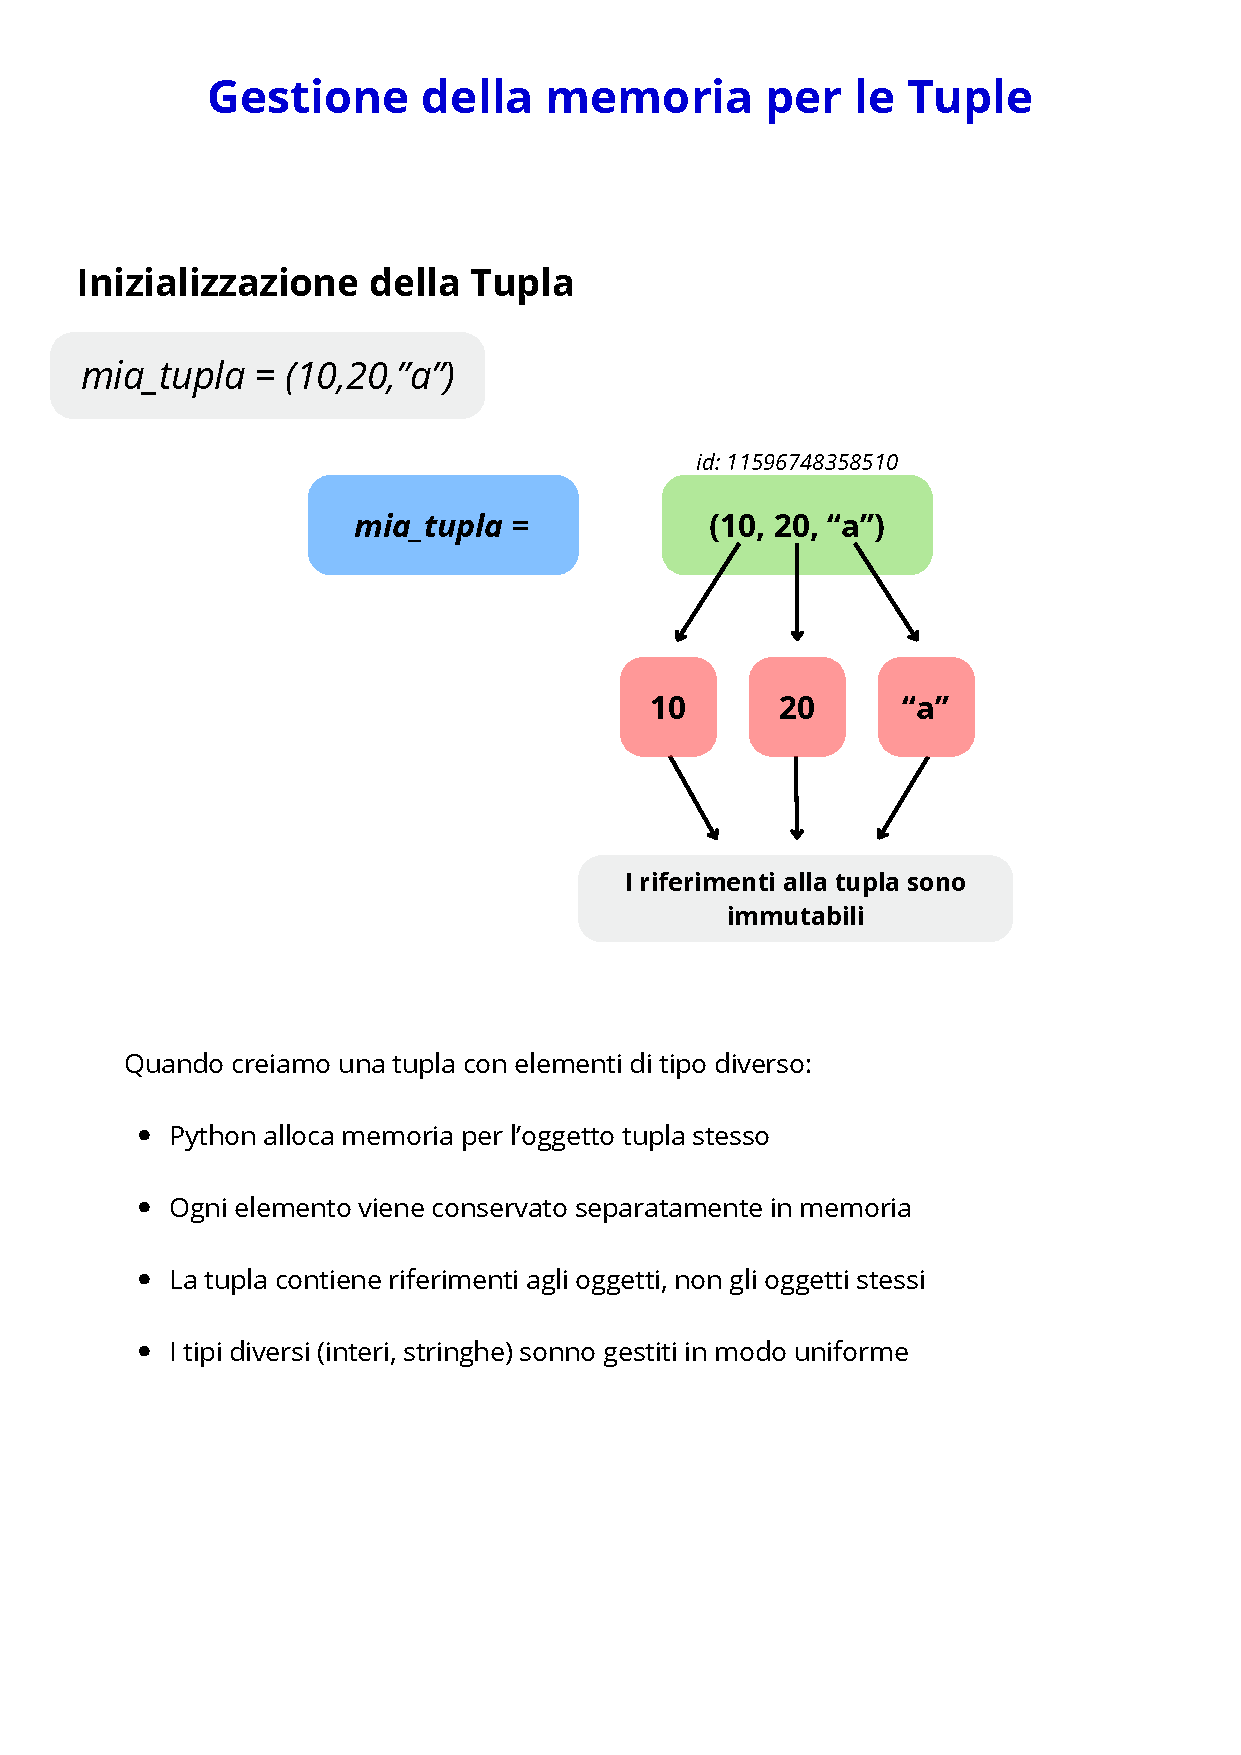
\includepdf[pages=-,scale=0.95,pagecommand={\thispagestyle{empty}},fitpaper=true]{pdf/Tuple.pdf}


\subsection{Esercizi Riassuntivi}
Come di consueto affrontiamo una serie di esercizi riassuntivi per familiarizzare con i concetti affrontati, alcuni esercizi possono sembrare banali, ma hanno lo scopo di far pratica con la sintassi, evitando gli errori comuni, altri sono strutturati in modo da generare errori in modo tale da familiarizzare con le diciture degli errori e capire cosa riportano.




\subsubsection{Esercizio 1: Creazione e sintassi Base delle Tuple}\label{Esercizio1Tuple}


\begin{lstlisting}
# Crea le seguenti tuple:
# Una tupla vuota
# Una tupla contenente solamente il numero 42
# Una tupla con i numeri da 1 a 5
# Una tupla mista con un numero, una stringa, un booleano
# Una tupla di stringhe
\end{lstlisting}

Per questo esercizio, ripassare le sezioni:
\begin{itemize}
    \item \hyperref[SintassiTuple]{Sintassi base Delle tuple. pag.\pageref{SintassiTuple}}
\end{itemize}


\subsubsection{Esercizio 2: Accesso agli Elementi (indicizzazione)}\label{Esercizio2Tuple}

\begin{lstlisting}
# Data la tupla
animali = ("cane", "gatto", "pesce", "uccello", "tartaruga")

# Stampare il primo elemento della tupla
# Stampare l'ultimo elemento tramite indicizzazione negativa
# Stampare il terzo elemento
# Stampare il penultimo elemento
# Cosa succede se provi ad accedere all'indice 10? Spiega l'errore
\end{lstlisting}

Per questo esercizio, ripassare le sezioni:
 \begin{itemize}
     \item \hyperref[TupleIndicizzazione]{Indicizzazione delle Tuple. pag.\pageref{TupleIndicizzazione}}
 \end{itemize}


 \subsubsection{Esercizio 3: Sclicing delle Tuple}\label{Esercizio3Tuple}
 \begin{lstlisting}
# Data la tupla
numeri = (0,1,2,3,4,5,6,7,8,9)

# Estrai i primi 3 elementi
# Estrai gli ultimi 4 elementi
# Estrai gli elementi dal 2 al 6 (inclusi)
# Estrai tutti gli elementi con indice pari
# Estrai tutti gli elementi in ordine inverso
# Estrai ogni secondo elemento a partire dal primo
 \end{lstlisting}

 Per questo esercizio, ripassare la sezione:
 \begin{itemize}
     \item \hyperref[SlicingTuple]{Slicing per le Tuple. pag\pageref{SlicingTuple}}
 \end{itemize}
 

 \subsubsection{Esercizio 4: Metodi per le Tuple}\label{Eserciozio4Tuple}
 \begin{lstlisting}
# Data la tupla 
frutti = ("mela", "banana", "mela", "arancia", "mela", "kiwi", "banana")

# Conta quante volte appare "mela" nella tupla
# Trova l'indice della prima occorrenza di "banana"
# Conta quante volte appare "pera"
# Trova la lunghezza deella tupla
# Verifica se "arancia" è presente nella tupla usando l'operatore "in" 
 \end{lstlisting}

 Per questo esercizio, ripassare la sezione:
 \hyperref[TabellaRiassuntiMetodiTuple]{Tabella riassuntiva dei metodi per le Tuple. pag\pageref{TabellaRiassuntiMetodiTuple}}



\subsubsection{Esercizio 5: Concatenazione delle Tuple}\label{Esercizio5ConcatenazioneTuple}
\begin{lstlisting}
# Date le tuple:
tuple1 = (1,2,3)
tuple2 = (4,5,6)

# Concatena le due tuple usando l'operatore + e salva il risultato in tuple3
# Moltiplica tuple1 per 3 usando l'operatore * e stampa il risultato
# Crea una nuova tupla concatenando (0,) con tuple1
# Crea una nuova tupla concatenando tuple2 con (7,)
\end{lstlisting}
 Per questo esercizio, ripassare la sezione:
 \begin{itemize}
     \item  \hyperref[ConcatenazioneTuple]{Concatenazione delle Tuple. pag\pageref{ConcatenazioneTuple}}
 \end{itemize}

 \subsubsection{Esercizio 6: Immutabilità delle Tuple}\label{Esercizio6ImmutabilitàTuple}
 \begin{lstlisting}
# Crea una tupla: coordinate = (10,20)
# Prova a modificare il primo elemento scrivendo coordinate[0] = 15
# Spiega l'errore che ottieni
# Dimostra come modificare una tupla, creandone una nuova
# Confronta questo comportamento con quello delle liste
 \end{lstlisting}

 Per questo esercizio, ripassare la sezione:
 \begin{itemize}
     \item  \hyperref[CaratteristicheTuple]{Caratteristiche delle Tuple. pag\pageref{CaratteristicheTuple}}
 \end{itemize}



 \subsubsection{Esercizio 7: Tuple Annidate}\label{EsercizioTupleAnnidate}
 \begin{lstlisting}
# Data la tupla 
coordinate = ((0,0),(1,1),(2,4),(3,9))

# Accedi alla seconda coppia di coordinate
# Accedi al valore "y" della terza coppia di coordinate
# Accedi al valore "x" della prima coppia di coordinate
# Conta quante coppie di coordinate ci sono
 \end{lstlisting}

 Per questo esercizio, ripassare la sezione:
 \hyperref[ConcatenazioneTuple]{Concatenazione delle Tuple. pag\pageref{ConcatenazioneTuple}}


 \subsubsection{Esercizio 8: Operazioni di Confronto}\label{Esercizio8ConfrontoTuple}
\begin{lstlisting}
# Date le tuple
a = (1, 2, 3)
b = (1, 2, 3)
c = (3, 2, 1)

# Verificare se a == b
# Verificare se a == c
# Verificare se a is b
# Spiegare la differenza tra == e is
\end{lstlisting}

Per questo esercizio, ripassare la sezione:
\hyperref[ConfrontoOperatoriListe]{Operatore Confronto. pag\pageref{ConfrontoOperatoriListe}}


\subsubsection{Esercizzio 9: Applicazione Pratica}\label{Esercizio9Tuple}
\begin{lstlisting}
# Inizializzazione di un sistema per memorizzare informazioni dei studenti

# Crea una tupla per rappresentare uno studente con: nome, eta', voto
# Crea una tupla contenente 3 studenti diversi
# Accedi alle informazioni del secondo studente
# Trova un modo per modificare alcuni studendi che potrebbero avere voti in sospeso
\end{lstlisting}


Per questo esercizio, ripassare le varie metodologie applicate alle tuple.
\begin{itemize}
    \item \hyperref[ConcatenazioneTuple]{Concatenazione. pag\pageref{ConcatenazioneTuple}}
    \item \hyperref[CaratteristicheTuple]{Caratteristiche delle Tuple. pag\pageref{CaratteristicheTuple}}
    \item \hyperref[TabellaRiassuntiMetodiTuple]{Tabella dei metodi per Tuple. pag\pageref{TabellaRiassuntiMetodiTuple}}
\end{itemize}



\subsection{Risoluzione Esercizi sulle Tuple}\label{RisoluzioneEserciziTuple}

\subsubsection{Risoluzione: \nameref{Esercizio1Tuple}}

\begin{lstlisting}
# Crea le seguenti tuple:
# Una tupla vuota
# Una tupla contenente solamente il numero 42
# Una tupla con i numeri da 1 a 5
# Una tupla mista con un numero, una stringa, un booleano
# Una tupla di stringhe



tupla_vuota = ()
print(type(tupla_vuota))

tupla_num = (42,)
print(type(tupla_num),tupla_num)

tuple_serie = (1,2,3,4,5)
print(type(tuple_serie),tuple_serie)

tupla_range = tuple(range(1,5+1))
print(tupla_range, type(tupla_range))

tupla_mista = ("a",23,True)
print(type(tupla_mista),tupla_mista)

stringa_tupla = tuple("python")
print(type(stringa_tupla), stringa_tupla)

tupla_stringhe = ("rosso", "verde", "blu")
print(type(tupla_stringhe), tupla_stringhe)
\end{lstlisting}


\subsubsection{Risoluzione: \nameref{Esercizio2Tuple}}

\begin{lstlisting}
#Data la tupla
animali = ("cane", "gatto", "pesce", "uccello", "tartaruga")
# Stampare il primo elemento della tupla
# Stampare l'ultimo elemento tramite indicizzazione negativa
# Stampare il terzo elemento
# Stampare il penultimo elemento
# Cosa succede se provi ad accedere all'indice 10? Spiega l'errore


print("primo elemento: ", animali[0])
print("ultimo elemento con indice negativo: ",animali[-1])
print("terzo elemento: ",animali[2])
print("penultimo elemento: ", animali[-2])
print("indice errato: ", animali[10])
\end{lstlisting}


\subsubsection{Risoluzione: \nameref{Esercizio3Tuple}}

\begin{lstlisting}
#Data la tupla
numeri = (0,1,2,3,4,5,6,7,8,9)
# Estrai i primi 3 elementi
# Estrai gli ultimi 4 elementi
# Estrai gli elementi dal 2 al 6 (inclusi)
# Estrai tutti gli elementi con indice pari
# Estrai tutti gli elementi in ordine inverso
# Estrai ogni secondo elemento a partire dal primo


#Primi 3
print(numeri[0:3])

#Ultimi 4
print(numeri[-4:])

#Dal 2 al 6
print(numeri[2:-3])

#Indice pari
print(numeri[::2])

#Ordine inverso
print(numeri[::-1])

#Ogni secondo elemento
print(numeri[0::2])
\end{lstlisting}


\subsubsection{Risoluzione: \nameref{Eserciozio4Tuple}}

\begin{lstlisting}
# Data la tupla
frutti = ("mela", "banana", "mela", "arancia", "mela", "kiwi", "banana")
# Conta quante volte appare "mela" nella tupla
# Trova l'indice della prima occorrenza di "banana"
# Conta quante volte appare "pera"

# Trova la lunghezza deella tupla
# Verifica se "arancia" e' presente nella tupla usando l'operatore "in"

#Contare quante volte appare mela
print(frutti.count("mela"))

#Trovare l'indice di banana
print(frutti.index("banana"))

#Contare quante volte appare pera
print(frutti.count("pera"))

#Trovare la lunghezza della tupla
print(len(frutti))

#Cercare se c'è arancia in frutti
print("arancia" in frutti)
\end{lstlisting}


\subsubsection{Risoluzione: \nameref{Esercizio5ConcatenazioneTuple}}

\begin{lstlisting}
# Date le tuple:
tuple1 = (1,2,3)
tuple2 = (4,5,6)
# Concatena le due tuple usando l'operatore + e salva il risultato in tuple3
# Moltiplica tuple1 per 3 usando l'operatore * e stampa il risultato
# Crea una nuova tupla concatenando (0,) con tuple1
# Crea una nuova tupla concatenando tuple2 con (7,)


tuple3 = tuple1 + tuple2
print(tuple3)

print(tuple1 * 3)

tupla0 = (0,) + tuple1
print(tupla0)

tupla4 =  tuple2 + (7,)
print(tupla4)

\end{lstlisting}

\subsubsection{Risoluzione: \nameref{Esercizio6ImmutabilitàTuple}}

\begin{lstlisting}
# Crea una tupla: coordinate = (10,20)
# Prova a modificare il primo elemento scrivendo coordinate[0] = 15
# Spiega l'errore che ottieni
# Dimostra come modificare una tupla, creandone una nuova
# Confronta questo comportamento con quello delle liste


# 1. Crea una tupla
coordinate = (10, 20)
print("Tupla originale:", coordinate)

# 2. Prova a modificare il primo elemento (questo causerà un errore!)
try:
    coordinate[0] = 15
except TypeError as e:
    print("ERRORE:", e)

# 3. Spiegazione dell'errore:
print("\nSpiegazione:")
print("L'errore 'tuple object does not support item assignment' significa che")
print("le tuple sono IMMUTABILI - non possono essere modificate dopo la creazione.")

# 4. Come 'modificare' una tupla creandone una nuova
print("\n4. 'Modifica' creando una nuova tupla:")
nuove_coordinate = (15, coordinate[1])
print("Coordinate originali:", coordinate)  # (10, 20) - invariata!
print("Nuove coordinate:", nuove_coordinate)  # (15, 20)

# 5. Confronto con le liste
print("\n5. Confronto con le liste:")
lista_coordinate = [10, 20]
print("Lista originale:", lista_coordinate)

lista_coordinate[0] = 15  # Questo funziona!
print("Lista modificata:", lista_coordinate)

print("\nRIASSUNTO:")
print("- TUPLE: immutabili, non si possono modificare")
print("- LISTE: mutabili, si possono modificare")

\end{lstlisting}


\subsubsection{Risoluzione: \nameref{EsercizioTupleAnnidate}}

\begin{lstlisting}
# Data la tupla
coordinate = ((0,0),(1,1),(2,4),(3,9))

print("Tupla coordinate:", coordinate)
print("Ogni elemento è una coppia (x, y)")
print()

# 1. Accedi alla seconda coppia di coordinate
print("1. Seconda coppia di coordinate:")
seconda_coppia = coordinate[1]
print("coordinate[1] =", seconda_coppia)

# 2. Accedi al valore "y" della terza coppia (il valore 4)
print("2. Valore 'y' della terza coppia:")
y_terza = coordinate[2][1]
print("coordinate[2][1] =", y_terza)

# 3. Accedi al valore "x" della prima coppia  
print("3. Valore 'x' della prima coppia:")
x_prima = coordinate[0][0]
print("coordinate[0][0] =", x_prima)

# 4. Conta quante coppie di coordinate ci sono
print("4. Numero di coppie:")
numero_coppie = len(coordinate)
print("len(coordinate) =", numero_coppie)

\end{lstlisting}


\subsubsection{Risoluzione: \nameref{Esercizio8ConfrontoTuple}}

\begin{lstlisting}
# Date le tuple
a = (1, 2, 3)
b = (1, 2, 3)
c = (3, 2, 1)

# Verificare se a == b
# Verificare se a == c
# Verificare se a is b
# Spiegare la differenza tra == e is


#Verifichiamo se a == b
print(a == b)

#Verifichiamo se a == c
print(a == c)

#Verifichiamo se a is b
print(a is b)

"""
Spiegazione dettagliata:

== (equality): Confronta il contenuto/valori

a == b -> True (stessi valori: 1,2,3)
a == c -> False (valori diversi: 1,2,3 vs 3,2,1)


is (identity): Confronta l'identità in memoria

a is b -> Solitamente False (oggetti separati)
Solo se puntano allo stesso oggetto in memoria restituisce True



Regola pratica:

Usa == per confrontare contenuti
Usa is per verificare se sono lo stesso oggetto

"""

\end{lstlisting}

\subsubsection{Risoluzione: \nameref{Esercizio9Tuple}}

\begin{lstlisting}
# Inizializzazione di un sistema per memorizzare informazioni dei studenti

# 1. Crea una tupla per rappresentare uno studente con: nome, età, voto 
# 2. Crea una tupla contenente 3 studenti diversi 
studenti = (("Mario", 19, 27), ("Luca", 18, 29), ("Giulia", 19, 30))

print("Sistema studenti:", studenti)


# 3. Accedi alle informazioni del secondo studente 
print("Secondo studente:", studenti[1])


# 4. Trova un modo per modificare alcuni studenti che potrebbero avere voti in sospeso
print("=== MODIFICA VOTI IN SOSPESO ===")


#Dato che la tupla puo' contenere anche delle liste lo studente con il voto in sospeso lo mettiamo dentro una lista, in modo tale da poterlo modificare
studenti = (["Mario", 19, 27], ("Luca", 18, 29), ("Giulia", 19, 30))

#In questo modo ora possiamo accedere allo studente e modificare il voto
    #Osserviamo che lo studente [0] risulta essere una lista
print(type(studenti[0]))

studenti[0][2]= 30

print(studenti[0])

#Ovviamente creare una struttura dove alcuni elementi sono liste e altri tuple, senza logiche evidenti, potrebbe confondere chi legge il codice, che deve controllare ogni volta che tipo type() e' ogni elemento per capire o meno se e' modificabile.
\end{lstlisting}

\newpage









%Sezione Dizionari
\subsection{Dizionari}\label{IncipitDizionari}

Fino ad adesso abbiamo affrontato come strutturare i dati tramite le liste e le tuple, in Python esiste anche un ulteriore metodo per strutturare i dati, i \textit{\textbf{dizionari.}}

A differenza delle liste e delle tuple, i \textit{\textbf{dizionari}} offrono una metodologia di collezione dei dati in più, quella di abbinare ogni valore a una chiave.

Si dichiarano tramite parentesi graffe \textit{\textbf{{}}} e come le liste possono contenere elementi di tipo diversi: \textit{Booleani, stringhe, interi, float.} Come per le liste esiste il metodo built-in di Python per dichiarare un dizionario: dict()

\vspace{0.5cm}
\textbf{Metodi Dichiarativi per Dizionari:}
\begin{lstlisting}
#Dichiarazione Dizionario tramite parentesi {}
dizionario = {
    "chiave1": valore1,
    "chiave2": valore2,
    "chiave3": valore3
}

#Dichiarazione tramite metodo dict()
dizionario_Dict = dict("chiave"=valore1, "chiave2"=valore2, "chiave3"=valore3)
\end{lstlisting}
\vspace{0.5cm}
Per quanto riguarda il metodo \textit{\textbf{dict(),}} bisogna approfondire alcuni aspetti, in quanto questo metodo ha alcune restrizioni, rispetto alla dichiarazione canonica.

\vspace{0.5cm}
\begin{lstlisting}
"""
Con {} puoi usare chiavi di qualsiasi tipo (anche numeri o tuple), mentre con dict() le chiavi devono essere stringhe valide come nomi di variabili (quindi niente spazi, accenti, ecc.).

Se vuoi creare un dizionario da una lista di coppie chiave-valore, dict() può essere comodo:
"""

coppie = [("nome", "Luca"), ("età", 30), ("città", "Milano")]
persona = dict(coppie)

\end{lstlisting}



\subsubsection{Chiavi - Valori}\label{ChiaveValoreDizionari}

Questa capacità di associare un valore a una determinata chiave fa sì che si possa costruire una mappa associativa, dove ogni elemento è costituito da una coppia chiave - valore, permettendo così un accesso rapido e efficiente ai dati, grazie alla peculiarità delle caratteristiche delle chiavi.

\subsubsection{Caratteristiche delle Chiavi}\label{CaratteristicheChiaviDict}
Come già accennato, la rapidità e l'efficienza che offrono i \textit{\textbf{dizionari}} sono date principalmente dalle caratteristiche che determinano le chiavi.


\begin{lstlisting}
#Esempio Dizionario
dizionario = {
    "chiave1":valore1,
    "chiave2":valore2,
    "chiave3":valore3
}
\end{lstlisting}


\vspace{0.5cm}
\begin{tcolorbox}[colback=blue!5!white,colframe=blue!75!black,title=Caratteristiche principali delle Chiavi]
\begin{itemize}
    \item \textbf{Hashabilità}: Devono avere un valore hash costante.
    
    \item \textbf{Immutabilità}: Non possono essere modificate dopo la creazione.
    
    \item \textbf{Unicità}: Ogni chiave appare una sola volta nel dizionario.
    
    \item \textbf{Confrontabilità}: Devono supportare l'operatore \textit{\textbf{==}} di uguaglianza.
    
    \item \textbf{Tipologia Libera}: Possono essere di qualsiasi tipo purché hashable.
    
\end{itemize}
\end{tcolorbox}


Vediamo, tramite esempi pratici, a cosa fanno riferimento queste caratteristiche.
\vspace{0.5cm}

\textbf{Hashabilità}
\begin{lstlisting}
# Le chiavi devono essere oggetti hashable
# Devono implementare il metodo __hash__()
# Il valore hash deve rimanere costante durante la vita dell'oggetto

print(f"Hash di 'ciao': {hash('ciao')}")    # Output -5659573120285894662
print(f"Hash di 42: {hash(42)}")            # Output 42
print(f"Hash di (1,2,3): {hash((1,2,3))}")  # Output 529344067295497451
\end{lstlisting}

\vspace{0.5cm}
\textbf{Immutabilità}
\begin{lstlisting}
# Le chiavi devono essere immutabili dopo la crezione
# Non possono essere modificate in-place
# Garantiscono che il valore hash rimanga stabile

dizionario = {}
chiave_stringa = "prodotto"
dizionario[chiave_stringa] = "Laptop"
# la chiave stringa non puo' essere modificata in-place
print(dizionario)      # Output {'prodotto': 'Laptop'}
\end{lstlisting}

\vspace{0.5cm}
\textbf{Unicità}
\begin{lstlisting}
# Ogni chiave puo' apparire una sola volta nel dizionario
# Se si inserisce una chiave esistente , il valore precedente viene sovrascritto
# L'unicita' è verificata tramite l'operatore ==

prodotti = {}

# Prima inserzione
prodotti["laptop"] = {"prezzo":800, "quantita":4}
print(f"Dopo prima inserzione: {prodotti}")

# Output Dopo prima inserzione: {'laptop': {'prezzo': 800, 'quantita': 4}}

# Seconda inserzione con stessa chiave - sovrascrive!
prodotti["laptop"] = {"prezzo": 750, "quantità": 3}
print(f"Dopo sovrascrittura: {prodotti}")
# Output Dopo sovrascrittura: {'laptop': {'prezzo': 750, 'quantità': 3}}


# Verifica che abbiamo sempre una sola chiave
print(f"Numero di chiavi: {len(prodotti)}")  
# Output Numero di chiavi: 1

# Anche con tipi numerici
numeri = {}
numeri[1] = "uno"
numeri[1.0] = "uno punto zero"  
# Output 1 == 1.0 in Python!

print(f"Chiavi numeriche: {numeri}")  
# Output {1: 'uno punto zero'}
print(f"1 == 1.0? {1 == 1.0}")  
# Output True
\end{lstlisting}


\vspace{0.5cm}
\textbf{Confrontabilità}
\begin{lstlisting}
# Le chiavi devono implementare il metodo __eq__()
# Permette di determinare se due chiavi sono identiche
# Usato per risolvere eventuali collisioni di hash

# Esempio 1: Numeri equivalenti
inventario = {}

# Inserimento con chiave intera
inventario[1] = "Un articolo"
print(f"Dopo inserimento con 1: {inventario}")

# Inserimento con chiave float equivalente
inventario[1.0] = "Un articolo (aggiornato)"  # 1 == 1.0!
print(f"Dopo inserimento con 1.0: {inventario}")
print(f"Numero di chiavi: {len(inventario)}")  # Solo 1 chiave!

# Verifica dell'uguaglianza
print(f"1 == 1.0? {1 == 1.0}")  # True
print(f"hash(1) == hash(1.0)? {hash(1) == hash(1.0)}")  # True

# Esempio 2: Tuple con contenuto identico
coordinate = {}

# Due tuple create separatamente ma con contenuto uguale
punto_a = (3, 4)
punto_b = (3, 4)

coordinate[punto_a] = "Prima posizione"
print(f"Dopo prima inserzione: {coordinate}")

coordinate[punto_b] = "Seconda posizione"  # Sovrascrive!
print(f"Dopo seconda inserzione: {coordinate}")

# Verifica dell'uguaglianza
print(f"punto_a == punto_b? {punto_a == punto_b}")  # True
print(f"punto_a is punto_b? {punto_a is punto_b}")  # Può essere True o False
print(f"hash(punto_a) == hash(punto_b)? {hash(punto_a) == hash(punto_b)}")  # True

# Esempio 3: Stringhe con contenuto identico
database = {}

# Stringhe create in modi diversi ma con contenuto uguale
chiave1 = "utente_001"
chiave2 = "utente" + "_" + "001"
chiave3 = f"utente_{1:03d}"

database[chiave1] = "Mario Rossi"
database[chiave2] = "Luigi Verdi"  # Sovrascrive Mario Rossi
database[chiave3] = "Anna Bianchi"  # Sovrascrive Luigi Verdi

print(f"Database finale: {database}")
print(f"Numero di utenti: {len(database)}")  # Solo 1!

# Verifica delle uguaglianze
print(f"chiave1 == chiave2? {chiave1 == chiave2}")  # True
print(f"chiave2 == chiave3? {chiave2 == chiave3}")  # True
print(f"Tutte le chiavi: '{chiave1}', '{chiave2}', '{chiave3}'")

# Esempio 4: Caso interessante con True/False e 1/0
configurazione = {}

# Bool e int equivalenti
configurazione[True] = "Modalità attiva"
configurazione[1] = "Valore uno"  # Sovrascrive True!

configurazione[False] = "Modalità disattiva" 
configurazione[0] = "Valore zero"  # Sovrascrive False!

print(f"Configurazione: {configurazione}")
print(f"True == 1? {True == 1}")    # True
print(f"False == 0? {False == 0}")  # True
\end{lstlisting}

\vspace{0.5cm}

\textbf{Tipologia libera}
\begin{lstlisting}
# Non esiste restrizione sul tipo di oggetto (basta che sia hashable)
# Possono coesistere chiavi di tipi diversi nello stesso dizionario
# Raccomandato mantenere coerenza per leggibilita'

# Dizionario con chiavi di tipi diversi - tutti nello stesso dizionario!
collezione_mista = {
    # Stringa come chiave
    "nome": "Mario Rossi",
    
    # Numero intero come chiave
    42: "La risposta universale",
    
    # Numero decimale come chiave
    3.14: "Pi greco approssimato",
    
    # Tupla come chiave
    (1, 2, 3): "Coordinate tridimensionali",
    
    # Valore booleano come chiave
    True: "Stato attivo",
    
    # None come chiave
    None: "Valore indefinito"
}

# Accesso alle diverse chiavi
print("Esempi di accesso con chiavi di tipi diversi:")
print(f"Nome: {collezione_mista['nome']}")
print(f"Numero: {collezione_mista[42]}")
print(f"Pi greco: {collezione_mista[3.14]}")
print(f"Coordinate: {collezione_mista[(1, 2, 3)]}")
print(f"Stato: {collezione_mista[True]}")
print(f"Indefinito: {collezione_mista[None]}")

# Esempio pratico: sistema di configurazione
configurazione_sistema = {
    # Chiavi stringa per impostazioni testuali
    "host": "localhost",
    "database": "app_principale",
    
    # Chiavi numeriche per valori numerici
    8080: "Porta del server",
    443: "Porta HTTPS",
    
    # Chiavi booleane per flag
    True: "Modalità di produzione attiva",
    False: "Modalità di debug disattiva",
    
    # Tupla per configurazioni composite
    ("cache", "redis"): "127.0.0.1:6379"
}

print("\nConfigurazione sistema:")
print(f"Host: {configurazione_sistema['host']}")
print(f"Porta HTTP: {configurazione_sistema[8080]}")
print(f"Produzione: {configurazione_sistema[True]}")
print(f"Cache Redis: {configurazione_sistema[('cache', 'redis')]}")

# Attenzione: comportamenti speciali con tipi misti
problemi_comuni = {}

# True e 1 sono considerati la stessa chiave!
problemi_comuni[True] = "Valore booleano"
problemi_comuni[1] = "Valore intero"  # Sovrascrive True!
print(f"\nProblema con True/1: {problemi_comuni}")  # Solo una chiave

# False e 0 sono considerati la stessa chiave!
problemi_comuni[False] = "Valore booleano falso"
problemi_comuni[0] = "Valore zero"  # Sovrascrive False!
print(f"Problema con False/0: {problemi_comuni}")  # Solo due chiavi totali

# Esempio di buona pratica: mantenere coerenza nei tipi
# BENE - chiavi tutte stringhe
anagrafica_coerente = {
    "nome": "Luigi",
    "cognome": "Bianchi", 
    "età": "25",  # Anche l'età come stringa per coerenza
    "città": "Roma"
}

# MENO LEGGIBILE - tipi misti senza motivo
anagrafica_confusa = {
    "nome": "Luigi",
    42: "Bianchi",  # Perche' 42 per il cognome?
    (1, 2): "25",   # Perche' tupla per l'età?
    True: "Roma"    # Perche' True per la città?
}

print(f"\nAnagrafica coerente: {anagrafica_coerente}")
print(f"Anagrafica confusa: {anagrafica_confusa}")

# Verifica della dimensione del dizionario
print(f"\nNumero di elementi in collezione_mista: {len(collezione_mista)}")
print(f"Numero di elementi in configurazione_sistema: {len(configurazione_sistema)}")
\end{lstlisting}

%Sezione Set
\subsection{Set}

In questo capitolo ci troviamo ad affrontare l'implementazione dei \textit{\textbf{set,}} la loro struttura rimarca la struttura dati matematica degli insiemi e con essa anche le operazioni annesse.

Come già consetudine anche in questo capitolo affronteremo la parte teorica, esploreremo i vari casi d'uso correlati di esempi pratici.

\subsection{Caretteristiche Fondamentali}\label{fondamentsSet}
Come già accennato ad inizio capitolo i \textit{\textbf{set}} si rifanno alla teoria degli insiemi matematici, quindi prima di esplorare i \textit{\textbf{set}} in Python è bene conoscere la teoria degli insiemi.

\subsubsection{Teoria degli insiemi}\label{TeoriadegliInsiemi}

In matematica un insieme rappresenta una collezione di oggetti, \textit{non ordinati, distinti}, ogni oggetto, (in matematichese denominato elemento) può appartenere o non all'insieme, senza possibilità di duplicazione o ordinamento intrinseco.

Una definizione formale stabilisce che due insiemi sono uguali se e solo se contengono esattamente gli stessi elementi, indipendentemente dall'ordine in cui questi sono disposti, stessa considerazione avviene in Python, dove l'identità della collezione dipende esclusivamente dal contenuto e non dalla sequenza di disposizione.

\subsubsection{Uguaglianza e Principio di Estensionalità}\label{EstensionalitàSet}

Il principio di estensionalità stabilisce che due insiemi sono uguali se e solo se contengono esattamente gli stessi elementi. Questo principio implica che l'ordine di enumerazione degli elementi è irrilevante per determinare l'identità dell'insieme, così come il numero di volte in cui un elemento viene menzionato. 


Gli insiemi {1, 2, 3}, {3, 1, 2}, e {1, 2, 3, 1} rappresentano la medesima entità matematica.
Questa proprietà fondamentale si traduce direttamente nel comportamento dei set Python, dove l'operatore di uguaglianza verifica la coincidenza degli elementi indipendentemente dall'ordine di inserimento o dalla presenza di tentativi di inserimento duplicati.


\subsubsection{Operazioni tra Insiemi}\label{OperazioniTraInsiemi}

Iniziamo ad affrontare le operazioni possibili tra insiemi, dato che sono equivalenti con le operazioni tra \textit{\textbf{set}} in Python.

\paragraph{Unione tra Insiemi}
L'unione di due insiemi A e B in matematica equivale all'insieme contenente tutti gli elementi che appartengono ad \textbf{A} e a \textbf{B}


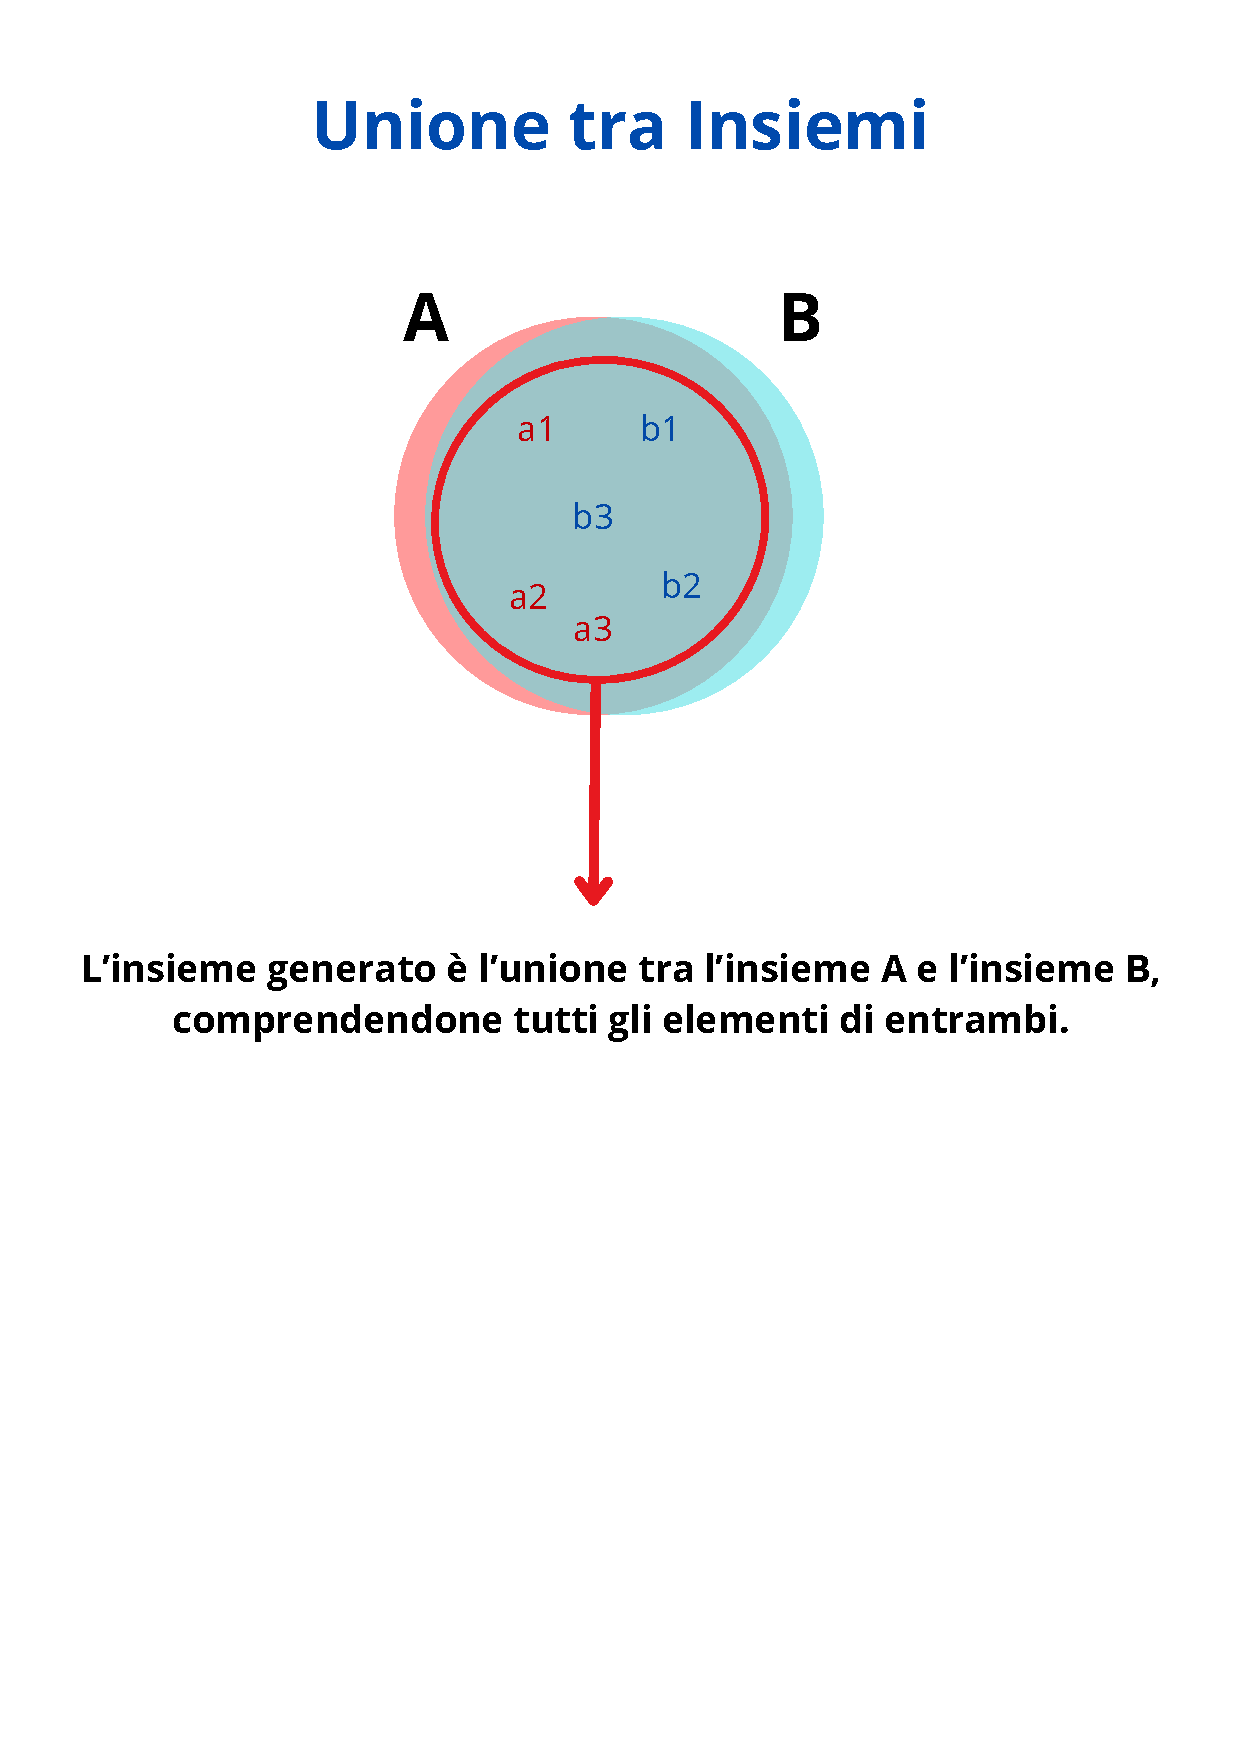
\includepdf[pages=-,scale=0.75,pagecommand={\thispagestyle{empty}},fitpaper=true]{pdf/Unione Insiemi.pdf}

\paragraph{Intersezione tra Insiemi}
L'intersezione tra insiemi, invece, comprende solo gli elementi comuni tra gli insiemi.

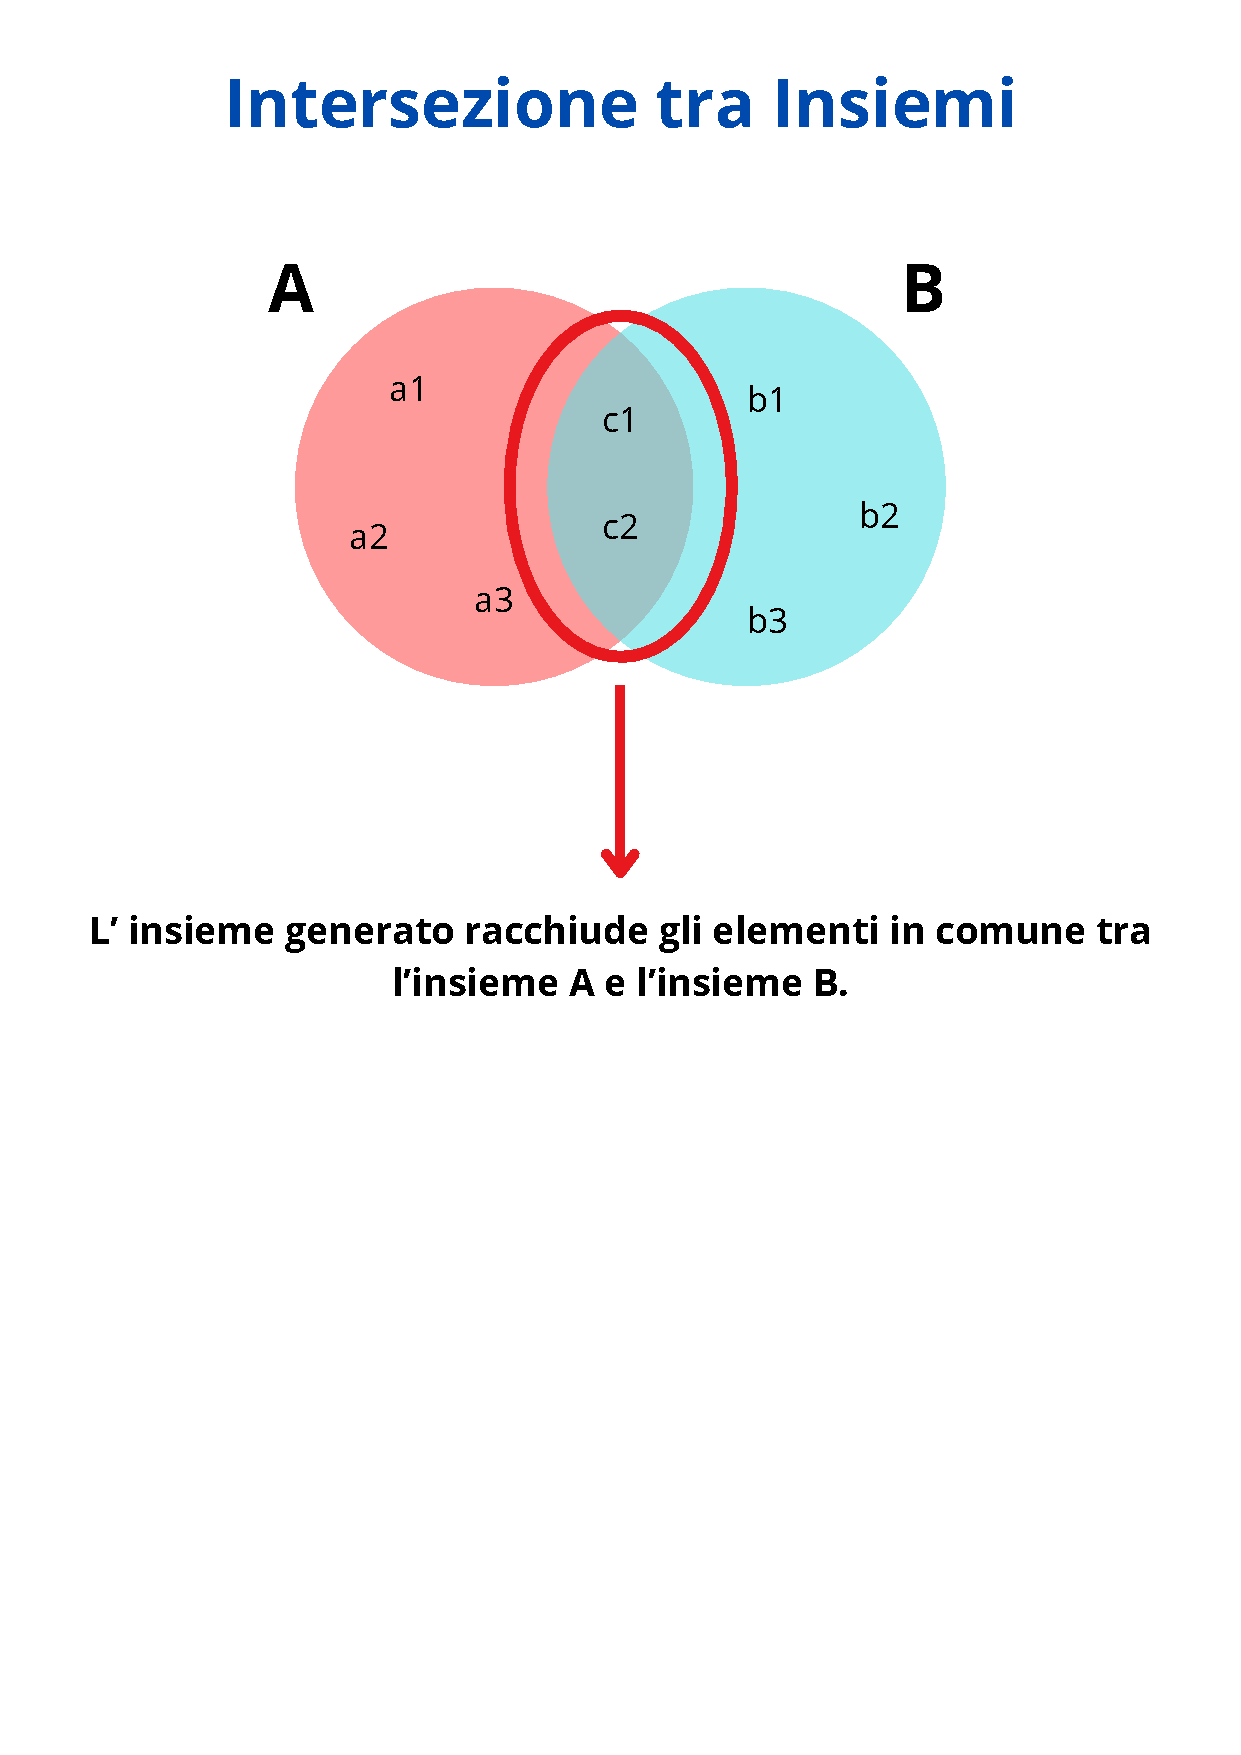
\includepdf[pages=-,scale=0.75,pagecommand={\thispagestyle{empty}},fitpaper=true]{pdf/Intetrsezione insiemi.pdf}


\paragraph{Differenza tra Insiemi}

L'operazione di differenza tra insiemi, A - B, non è altro che l'insieme contenente tutti gli elementi che appartengono ad A ma non a B



Un'altra operazione in comune tra i \textit{\textbf{set}} e gli insiemi matematici è quella della differenza simmetrica tra insiemi, come è facile intuire dal nome dell'operazione, l'insieme risultante sarà dato soltanto dagli elementi non comuni tra gli insiemi esaminati.

\end{document}
